%Template para TCC CIC UFRGS
%Author: Lucas Schnorr (Adaptado para overleaf por Rubens dos Santos)

% exemplo genérico de uso da classe iiufrgs.cls
% $Id: iiufrgs.tex,v 1.1.1.1 2005/01/18 23:54:42 avila Exp $
% 
% This is an example file and is hereby explicitly put in the
% public domain.
% 
\documentclass[ecp,tc]{iiufrgs}
% Para usar o modelo, deve-se informar o programa e o tipo de documento.
% Programas :
% * cic       -- Graduação em Ciência da Computação
% * ecp       -- Graduação em Ciência da Computação
% * ppgc      -- Programa de Pós Graduação em Computação
% * pgmigro   -- Programa de Pós Graduação em Microeletrônica
% 
% Tipos de Documento:
% * tc                -- Trabalhos de Conclusão (apenas cic e ecp)
% * diss ou mestrado  -- Dissertações de Mestrado (ppgc e pgmicro)
% * tese ou doutorado -- Teses de Doutorado (ppgc e pgmicro)
% * ti                -- Trabalho Individual (ppgc e pgmicro)
% 
% Outras Opções:
% * english    -- para textos em inglês
% * openright  -- Força início de capítulos em páginas ímpares (padrão da
% biblioteca)
% * oneside    -- Desliga frente-e-verso
% * nominatalocal -- Lê os dados da nominata do arquivo nominatalocal.def


% Use unicode
\usepackage[utf8]{inputenc}   % pacote para acentuação

% Necessário para incluir figuras
\usepackage{graphicx}         % pacote para importar figuras

\usepackage{times}            % pacote para usar fonte Adobe Times
% \usepackage{palatino}
% \usepackage{mathptmx}       % p/ usar fonte Adobe Times nas fórmulas

\usepackage{amsmath,amssymb}  % pacotes para ambientes e símbolos matemáticos

\usepackage[alf,abnt-emphasize=bf]{abntex2cite}	% pacote para usar citações abnt

% --- PACOTES ADICIONADOS PARA O DESENHO DAS MATRIZES ---
\usepackage{tikz}
\usepackage[normalem]{ulem}     % texto riscado (\sout) nas revisões do capítulo
\usetikzlibrary{decorations.pathreplacing, calc, positioning}


% 
% Informações gerais
% 
\title{Hardware Accelerator for Matrix Inversion in Decentralized Massive MIMO LMMSE Equalization Under Colored Noise}

\author{de Vargas}{Juliana Rodrigues}
% alguns documentos podem ter varios autores:
% \author{Flaumann}{Frida Gutenberg}
% \author{Flaumann}{Klaus Gutenberg}

% orientador e co-orientador são opcionais (não diga isso pra eles :))
\advisor[Prof.~Dr.]{Lamport}{Leslie}
\coadvisor[Prof.~Dr.]{Knuth}{Donald Ervin}

% a data deve ser a da defesa; se nao especificada, são gerados
% mes e ano correntes
% \date{maio}{2001}

% o local de realização do trabalho pode ser especificado (ex. para TCs)
% com o comando \location:
% \location{Itaquaquecetuba}{SP}

% itens individuais da nominata podem ser redefinidos com os comandos
% abaixo:
% \renewcommand{\nominataReit}{Prof\textsuperscript{a}.~Wrana Maria Panizzi}
% \renewcommand{\nominataReitname}{Reitora}
% \renewcommand{\nominataPRE}{Prof.~Jos{\'e} Carlos Ferraz Hennemann}
% \renewcommand{\nominataPREname}{Pr{\'o}-Reitor de Ensino}
% \renewcommand{\nominataPRAPG}{Prof\textsuperscript{a}.~Joc{\'e}lia Grazia}
% \renewcommand{\nominataPRAPGname}{Pr{\'o}-Reitora Adjunta de P{\'o}s-Gradua{\c{c}}{\~a}o}
% \renewcommand{\nominataDir}{Prof.~Philippe Olivier Alexandre Navaux}
% \renewcommand{\nominataDirname}{Diretor do Instituto de Inform{\'a}tica}
% \renewcommand{\nominataCoord}{Prof.~Carlos Alberto Heuser}
% \renewcommand{\nominataCoordname}{Coordenador do PPGC}
% \renewcommand{\nominataBibchefe}{Beatriz Regina Bastos Haro}
% \renewcommand{\nominataBibchefename}{Bibliotec{\'a}ria-chefe do Instituto de Inform{\'a}tica}
% \renewcommand{\nominataChefeINA}{Prof.~Jos{\'e} Valdeni de Lima}
% \renewcommand{\nominataChefeINAname}{Chefe do \deptINA}
% \renewcommand{\nominataChefeINT}{Prof.~Leila Ribeiro}
% \renewcommand{\nominataChefeINTname}{Chefe do \deptINT}

% A seguir são apresentados comandos específicos para alguns
% tipos de documentos.

% Relatório de Pesquisa [rp]:
% \rp{123}             % numero do rp
% \financ{CNPq, CAPES} % orgaos financiadores

% Trabalho Individual [ti]:
% \ti{123}     % numero do TI
% \ti[II]{456} % no caso de ser o segundo TI

% Monografias de Especialização [espec]:
% \espec{Redes e Sistemas Distribuídos}      % nome do curso
% \coord[Profa.~Dra.]{Weber}{Taisy da Silva} % coordenador do curso
% \dept{INA}                                 % departamento relacionado

% 
% palavras-chave
% iniciar todas com letras minúsculas, exceto no caso de abreviaturas
% 
\keyword{formatação eletrônica de documentos}
\keyword{\LaTeX}
\keyword{ABNT}
\keyword{UFRGS}

%\settowidth{\seclen}{1.10~}

% 
% inicio do documento
% 
\begin{document}

% folha de rosto
% às vezes é necessário redefinir algum comando logo antes de produzir
% a folha de rosto:
% \renewcommand{\coordname}{Coordenadora do Curso}
\maketitle

% dedicatoria
% \clearpage
% \begin{flushright}
%     \mbox{}\vfill
%     {\sffamily\itshape
%       ``If I have seen farther than others,\\
%       it is because I stood on the shoulders of giants.''\\}
%     --- \textsc{Sir~Isaac Newton}
% \end{flushright}

% agradecimentos
%\chapter*{Agradecimentos}
%Agradeço ao \LaTeX\ por não ter vírus de macro\ldots



% resumo na língua do documento
\begin{abstract}
    Este documento é um exemplo de como formatar documentos para o
    Instituto de Informática da UFRGS usando as classes \LaTeX\
    disponibilizadas pelo UTUG\@. Ao mesmo tempo, pode servir de consulta
    para comandos mais genéricos. \emph{O texto do resumo não deve
      conter mais do que 500 palavras.}
\end{abstract}

% resumo na outra língua
% como parametros devem ser passados o titulo e as palavras-chave
% na outra língua, separadas por vírgulas
\begin{englishabstract}{Using \LaTeX\ to Prepare Documents at II/UFRGS}{Electronic document preparation. \LaTeX. ABNT. UFRGS}
    This document is an example on how to prepare documents at II/UFRGS
    using the \LaTeX\ classes provided by the UTUG\@. At the same time, it
    may serve as a guide for general-purpose commands. \emph{The text in
      the abstract should not contain more than 500~words.}
\end{englishabstract}

% lista de figuras
\listoffigures

% lista de tabelas
\listoftables

% lista de abreviaturas e siglas
% o parametro deve ser a abreviatura mais longa
\begin{listofabbrv}{QuaDRiGa}
    \item[3GPP] 3rd Generation Partnership Project
    \item[5G] Quinta geração de redes móveis
    \item[AoA] Angle of Arrival
    \item[AoD] Angle of Departure
    \item[AWGN] Additive White Gaussian Noise
    \item[BCD] Block Coordinate Descent
    \item[BS] Base Station
    \item[DM-RS] Demodulation Reference Signal
    \item[DU] Distributed Unit
    \item[FR1] Frequency Range 1
    \item[FR2] Frequency Range 2
    \item[HST] High Speed Train
    \item[InF] Indoor Factory
    \item[InH] Indoor Hotspot
    \item[IoT] Interference over Thermal
    \item[ITU] International Telecommunication Union
    \item[LMMSE] Linear Minimum Mean Square Error
    \item[LoS] Line of Sight
    \item[MIMO] Multiple-Input Multiple-Output
    \item[MMSE] Minimum Mean Square Error
    \item[NLoS] Non-Line of Sight
    \item[NR] New Radio
    \item[O2I] Outdoor-to-Indoor
    \item[OFDM] Orthogonal Frequency Division Multiplexing
    \item[PRB] Physical Resource Block
    \item[QAM] Quadrature Amplitude Modulation
    \item[QPSK] Quadrature Phase Shift Keying
    \item[QuaDRiGa] Quasi-Deterministic Radio Channel Generator
    \item[RB] Resource Block
    \item[RE] Resource Element
    \item[RMa] Rural Macro-cell
    \item[SCS] Subcarrier Spacing
    \item[SER] Symbol Error Rate
    \item[SNR] Signal-to-Noise Ratio
    \item[TR] Technical Report
    \item[TS] Technical Specification
    \item[UE] User Equipment
    \item[ULA] Uniform Linear Array
    \item[UMa] Urban Macro-cell
    \item[UMi] Urban Micro-cell
    \item[UPA] Uniform Planar Array
    \item[ZF] Zero-Forcing
\end{listofabbrv}

% idem para a lista de símbolos
% \begin{listofsymbols}{$\alpha\beta\pi\omega$}
%     \item[$\sum{\frac{a}{b}}$] Somatório do produtório
%     \item[$\alpha\beta\pi\omega$] Fator de inconstância do resultado
% \end{listofsymbols}

% sumario
\tableofcontents

% aqui comeca o texto propriamente dito

% introducao
\chapter{Introdução}

\section{Figuras e tabelas}

% e aqui vai a parte principal
% 
% \chapter{Estado da arte}
% \chapter{Mais estado da arte}
% \chapter{A minha contribuição}
% \chapter{Prova de que a minha contribuição é válida}
% \chapter{Conclusão}

\chapter{Fundamentação Teórica}


% =====================================================================
\section{Sistemas MIMO}\label{sec:sistemas-MIMO}
% =====================================================================
\subsection{Uplink}\label{subsec:uplink}
\textcolor{red}{Este trabalho considera o \textit{uplink} de um sistema MIMO (\textit{Multiple-Input Multiple-Output}) massivo, em que $K$ Equipamentos de Usuário (UEs, \textit{User Equipments}) alvo, cada um com uma antena, transmitem dados para uma Estação Base (BS, \textit{Base Station}) com $M$ antenas, sendo $M \gg K$ \cite{zhao2025jsac}. Os UEs são atendidos ao mesmo tempo, nos mesmos recursos de tempo e frequência \cite{zhao2025jsac}.}

\textcolor{red}{O sistema segue o 5G NR (\textit{New Radio}), a tecnologia de acesso sem fio da quinta geração de redes móveis (5G) \cite[p.~2]{lin-lee-5g}. O NR é especificado pelo 3GPP (\textit{3rd Generation Partnership Project}) em um conjunto de normas técnicas, como a TS 38.211, que define os canais físicos e a modulação \cite{3gpp-ts38211}, e a TS 38.104, que define a transmissão e a recepção da BS \cite{3gpp-ts38104}. O NR divide o espectro em duas faixas de frequência: FR1 (\textit{Frequency Range} 1), de 410 MHz a 7125 MHz, e FR2, de 24250 MHz a 52600 MHz \cite[Tab.~5.1-1]{3gpp-ts38104}.}

\subsection{Símbolos e constelação}\label{subsec:simbolos}
\textcolor{red}{Cada UE transmite símbolos de uma constelação de modulação, como a 16-QAM (\textit{Quadrature Amplitude Modulation}) \cite{zhao2025jsac}. A energia média por símbolo é $E_s$ \cite{zhao2025jsac}.}

\textcolor{red}{No NR, esses símbolos são transmitidos com OFDM (\textit{Orthogonal Frequency Division Multiplexing}). O espaçamento entre subportadoras (SCS, \textit{Subcarrier Spacing}) depende da numerologia $\mu$, com $\Delta f = 2^{\mu}\cdot 15$ kHz \cite[Tab.~4.2-1]{3gpp-ts38211}. Por exemplo, $\mu=1$ corresponde a 30 kHz, e $\mu=3$ corresponde a 120 kHz.}

\textcolor{red}{No tempo, as transmissões são organizadas em quadros de 10 ms, e cada quadro tem dez subquadros de 1 ms \cite[Sec.~4.3.1]{3gpp-ts38211}. O slot é a divisão do subquadro usada na transmissão. Com prefixo cíclico normal, cada slot tem 14 símbolos OFDM, e cada subquadro tem $2^{\mu}$ slots \cite[Tab.~4.3.2-1]{3gpp-ts38211}. Assim, um slot dura 0,5 ms com $\mu=1$ e 0,125 ms com $\mu=3$.}

\textcolor{red}{A grade de recursos combina subportadoras, na frequência, e símbolos OFDM, no tempo. Cada elemento dessa grade é um elemento de recurso (RE, \textit{Resource Element}), que corresponde a uma subportadora em um símbolo OFDM \cite[Sec.~4.4.3]{3gpp-ts38211}. Um bloco de recursos (RB, \textit{Resource Block}) tem 12 subportadoras consecutivas na frequência \cite[Sec.~4.4.4.1]{3gpp-ts38211}. Os blocos de recursos físicos (PRBs, \textit{Physical Resource Blocks}) são os RBs usados dentro da parte da banda configurada para a transmissão \cite[Sec.~4.4.4.4]{3gpp-ts38211}.}

\subsection{Relação sinal-ruído}

\subsection{Modelo de canal}
\label{sec:modelo-canal}
% CONTEÚDO  O que o canal representa; modelos determinísticos e
%           estocásticos; desvanecimento; bloco de coerência; arranjos de
%           antenas; modelo 3GPP, QuaDRiGa e cenários.
% TEXTO     0.channel-modelling.tex (inteiro);
%           1-noise-and-constraints.tex, "Multipath, desvanecimento..." e
%           "Bloco de Coerência" (vazias);
%           constraints/rascunho_bloco_canal.tex (partes 1 e 2; ajustar o tom).
% ESTADO    parcial
A avaliação de um sistema de MIMO massivo precisa de um modelo que represente o canal com as principais características de um arranjo com muitas antenas. Esse modelo deve considerar a geometria do arranjo de antenas, a correlação espacial entre as respostas de canal de diferentes antenas e as características físicas do ambiente, como a localização e orientação das \sout{Estações Base (BSs) e dos Equipamentos de Usuário (UEs.)} \textcolor{red}{BSs e dos UEs}. 

\subsubsection{Tipos de modelo de canal}
Existem dois tipos principais de modelo de canal: determinísticos ou estocásticos. O modelo determinístico produz sempre o mesmo resultado sob as mesmas condições, pois depende de um ambiente específico com parâmetros fixos, como a localização dos transmissores, receptores, espalhadores e refletores de sinal. Exemplos desse modelo são o ray–tracing e medições reais de canal em campo. Nesse modelo há desvantagem para a reprodução de resultados, que exige o acesso aos dados de medição específicos do canal ou modelos 3D de prédios, que nem sempre estão disponíveis. 

Modelos estocásticos são independentes de um ambiente em particular e generalizam o comportamento do canal a partir de propriedades estatísticas selecionadas. Eles podem ser divididos em três categorias:

\begin{itemize}
  \item Baseados em correlação: Nos modelos baseados em correlação as respostas do canal seguem uma distribuição gaussiana com média zero, definidas por meio de matrizes de correlação. Um exemplo é o correlated Rayleigh fading model, que considera um desvanecimento plano em frequência, ou seja, que todos os componentes multi-path chegam à antena com o mesmo delay. Esse modelo é suficiente para uma análise dentro de um bloco de coerência \sout{(PRB)} \textcolor{red}{(um PRB, na frequência, durante $T_c$, no tempo)}, em que o canal é considerado constante.
  \item Paramétricos: Esses modelos definem distribuições estatísticas para o número de espalhadores,  atrasos, potências e ângulos de chegada e saída (AoA/AoD). Eles não consideram a geometria do ambiente, por isso não abrangem a análise da evolução temporal do canal que acontece com a movimentação dos \sout{Equipamentos de Usuário} \textcolor{red}{UEs}.
  \item Baseados em geometria: Esses modelos equilibram as características dos modelos estocásticos e determinísticos. Eles definem uma distribuição da localização física dos espalhadores de sinal ao redor dos transmissores e receptores. Os caminhos de propagação do canal são modelados a partir da localização dos espalhadores de uma maneira quase-determinística (quasi-deterministic). Um modelo quase-determinístico define um processo regido por leis fixas mas com uma margem de aleatoriedade dada por ruído e/ou variabilidade. 
\end{itemize} 

\subsubsection{Multipath, desvanecimento...}
\subsubsection{Bloco de Coerência}\label{subsec:bloco-coerencia}
% O setup de simulação se apoia aqui: W é reaproveitado para vários símbolos.
O tempo de coerência \(T_c\) corresponde ao intervalo durante o qual o canal pode ser considerado aproximadamente constante. Seu valor é calculado a partir do deslocamento Doppler máximo \(f_D\), pela expressão \(T_c=1/(8f_D)\) \cite{tse-viswanath}. Durante cada bloco de coerência, o canal e a matriz de covariância do ruído são considerados constantes, permitindo reutilizar a matriz de equalização \(\mathbf W\) ao longo desse intervalo \cite{zhao2025jsac}.

As condições de teste seguem os cenários de propagação definidos no Anexo G da norma 3GPP TS 38.104 \cite{3gpp-ts38104}. Para os cálculos, são adotados \sout{espaçamentos entre subportadoras (SCS)} \textcolor{red}{SCS} de 30 kHz em FR1 e 120 kHz em FR2 \cite[Tabs.~5.3.5-1 e 5.3.5-2]{3gpp-ts38104}. Considerando os 14 símbolos OFDM por slot \cite[Tab.~4.3.2-1]{3gpp-ts38211}, a Tabela~\ref{tab:tempo-coerencia} apresenta o tempo de coerência e o número de símbolos OFDM completos contidos nesse intervalo para cada condição de teste. A classificação de mobilidade típica baseia-se nos cenários de uso do 5G descritos pela ITU \cite[pp.~11, 14]{itu-m2083}.



\begin{table}[htbp]
\caption{\textcolor{red}{Tempo de coerência de cada condição de teste.}}
\label{tab:tempo-coerencia}
\centering
\footnotesize
\renewcommand{\arraystretch}{1.2}
\begin{tabular}{|l|p{4.2cm}|r|r|r|r|r|}
\hline
Condição de teste & \raggedright Mobilidade típica & $f_D$ (Hz) & $v$ (km/h) & SCS (kHz) & $T_c$ (ms) & Símb. OFDM \tabularnewline
\hline
TDLA30-5 (FR1) & \raggedright Baixa: \textit{hotspot}, \textit{indoor} & 5 & 1,5 & 30 & 25,0000 & 700 \tabularnewline
TDLA30-10 (FR1) & \raggedright Baixa: \textit{hotspot}, \textit{indoor} & 10 & 3,1 & 30 & 12,5000 & 350 \tabularnewline
TDLA30-75 (FR2) & \raggedright Baixa: \textit{hotspot}, \textit{indoor} & 75 & 2,9 & 120 & 1,6667 & 186 \tabularnewline
TDLA30-300 (FR2) & \raggedright Média a alta: área ampla, carros & 300 & 11,6 & 120 & 0,4167 & 46 \tabularnewline
TDLC300-100 (FR1) & \raggedright Média a alta: área ampla, carros & 100 & 30,8 & 30 & 1,2500 & 35 \tabularnewline
TDLB100-400 (FR1) & \raggedright Média a alta: área ampla, carros & 400 & 123,3 & 30 & 0,3125 & 8 \tabularnewline
HST350 (FR1) & \raggedright Alta: trem de alta velocidade & 2334 & 350 & 30 & 0,0536 & 1 \tabularnewline
HST500 (FR1) & \raggedright Alta: trem de alta velocidade & 3334 & 500 & 30 & 0,0375 & 1 \tabularnewline
\hline
\end{tabular}
\end{table}
% FONTE: f_D: TS 38.104 v16.4.0, Tab. G.2.2-1 e G.2.2-2 (p. 241), G.3-1 e G.3-2 (p. 252, SCS 30 kHz);
%        T_c = 1/(4 D_s): Tse e Viswanath, Eq. (2.44), p. 31; D_s = 2 f_c v/c e T_c = c/(8 f_c v): p. 70;
%        SCS: TS 38.104 Tab. 5.3.5-1 (n78) e 5.3.5-2 (n257); 14 símbolos/slot: TS 38.211 Tab. 4.3.2-1.
%        v (TDL): v = f_D c / f_c, Tse e Viswanath p. 70; f_c: TS 38.104 Tab. 5.2-1 (n78) e 5.2-2 (n257).
%        v (HST): TS 38.104 Tab. G.3-1 e G.3-2. NOTA: pela fórmula, 2334 Hz a 3,5 GHz daria ~720 km/h;
%        a norma deriva o f_d de HST para outras bandas e avisa que, em frequências menores, a velocidade
%        suportada é maior (Sec. G.3, p. 250).
%        Mobilidade: ITU-R M.2083-0, p. 4 (carros e trens), p. 11 (hotspot: baixa; área ampla: média a alta), p. 14 (até 500 km/h,
%        trens), p. 15. A associação condição -> categoria é deste trabalho (coluna do CSV).
%        Valores: software/Restrições - Parâmetros.csv, linhas 15-24.

\subsubsection{Arranjo de canal} 

A escolha dos arranjos de antena (ou seja, suas distribuições no espaço) dependem do caso de uso, da frequência dos portadores e da área de cobertura. Os arranjos podem ser organizados em geometrias lineares (Uniform Linear Array - ULA), planares (Uniform Planar Array - UPA) ou em geometrias cilíndricas. Modelos lineares e planares separam os UEs baseados na elevação ou posição azimutal, enquanto os cilíndricos conseguem trabalhar nos dois domínios ao mesmo tempo. Para cenários urbanos, o arranjo cilíndrico é mais adequado, pois permite a representação dos UEs em diferentes localizações e andares de prédios. 

\subsubsection{Modelo 3GPP e Simulador QuaDRiGa}

Linha de Visada (Line of Sight - LoS) é o trajeto livre de obstáculos que permite a visão direta entre dois pontos. Não é realista representar os caminhos de propagação apenas como linha de visada. A 3GPP definiu para sistemas MIMO um modelo estocástico baseado em geometria que representa um misto de caminhos de propagação NLos e LoS. Esse modelo une um layout determinístico do sistema MIMO (ocalização das BS e UE, orientação das antenas, dependência angular da intensidade das ondas de rádio transmitidas ou recebidas, frequência de subportadoras) e um conjunto de parâmetros aleatórios de larga escala gerados por distribuições estatísticas obtidas a partir de medições de canal. O simulador de canal de código aberto QuaDRiGa (Quasi-Deterministic Radio Channel Generator) implementa o modelo 3GPP 3D MIMO, e é o simulador utilizado neste trabalho. 



\subsubsection{Cenário de propagação}
% A frase "este trabalho usa o cenário UMa NLOS" vai para o setup.
Um cenário de propagação descreve um conjunto de parâmetros estatísticos para um tipo de ambiente. Dentre os modelos de cenário, o trabalho utiliza o 3GPP NR (\sout{TR 39.901} \textcolor{red}{TR 38.901}), \textcolor{red}{[que modela os parâmetros para o New Radio, que é uma frequencia maior, pior caso]}. Os ambientes do modelo \sout{3G-- 38.901} \textcolor{red}{3GPP TR 38.901} podem ter as seguintes características: 

\begin{itemize}
  \item \sout{Uma} \textcolor{red}{UMa} (\textit{Urban Macro-cell}): cidade densa, com antenas acima dos telhados. 
  \item \sout{Umi} \textcolor{red}{UMi} (\textit{Urban Micro-cell}): cidade densa, com uma antena pequena abaixo dos telhados, no nível da rua. 
  \item RMa (\textit{Rural Macro-cell}): área rural, com células grandes. 
  \item InH (\sout{\textit{Indoor Office}} \textcolor{red}{\textit{Indoor Hotspot}}): dentro de prédios, como escritórios.
  \item InF (\textit{Indoor Factory}): dentro de galpões de fábrica. 
\end{itemize}


Além disso, cada ambiente pode ter variações: 

\begin{itemize}
  \item LOS/NLOS: com ou sem visada direta entre antena e usuário. 
  \item O2I (\textit{Outdoor-to-Indoor}): antena do lado de fora e usuário dentro de prédio.         
\end{itemize}


Cada cenário do modelo é definido por um arquivo de configuração. A tabela \ref{tab:cenarios_38901} resume os cenários do modelo. Este trabalho usa o cenário \texttt{3GPP\_\allowbreak{}38.901\_\allowbreak{}UMa\_\allowbreak{}NLOS}, que representa uma macrocélula urbana (\textit{Urban Macro} - UMa) sem linha de visada (NLos) entre a BS e os UEs. 


\begin{table}[htbp]
\caption{Cenários do modelo 3GPP 38.901 no QuaDRiGa.}
\label{tab:cenarios_38901}
\centering
\footnotesize
\renewcommand{\arraystretch}{1.2}
\begin{tabular}{|p{3.6cm}|p{4.4cm}|p{5.2cm}|}
\hline
\raggedright Cenário & \raggedright Lugar & \raggedright Dados do manual \tabularnewline
\hline
\raggedright \texttt{3GPP\_\allowbreak{}38.901\_\allowbreak{}UMa} & \raggedright Cidade densa, antena no alto do prédio & \raggedright Célula de até $\sim$1 km, BS a 25 m, usuário de 1,5 a 22,5 m \tabularnewline
\hline
\raggedright \texttt{3GPP\_\allowbreak{}38.901\_\allowbreak{}UMi} & \raggedright Cidade densa, antena na rua, abaixo dos telhados & \raggedright Célula de até $\sim$200 m, BS a 10 m \tabularnewline
\hline
\raggedright \texttt{3GPP\_\allowbreak{}38.901\_\allowbreak{}RMa} & \raggedright Área rural & \raggedright Célula de até $\sim$10 km, BS de 10 a 150 m \tabularnewline
\hline
\raggedright \texttt{3GPP\_\allowbreak{}38.901\_\allowbreak{}Indoor} & \raggedright Escritório, como Wi-Fi ou femtocélula & \raggedright BS a 3 m, usuário a 1 m. Tem dois tipos, \textit{mixed office} e \textit{open office}, que só mudam a probabilidade de LOS. \tabularnewline
\hline
\raggedright \texttt{3GPP\_\allowbreak{}38.901\_\allowbreak{}InF} & \raggedright Galpão de fábrica com máquinas, linhas de montagem e prateleiras & \raggedright Versões NLOS por densidade de obstáculos (D: denso, S: esparso) e altura da BS (H: alta, L: baixa): DH, DL, SH e SL \tabularnewline
\hline
\end{tabular}
\legend{Fonte: manual do QuaDRiGa.} % TODO citar QuaDRiGa (Seção 2.5, Tabela 21, p. 108)
\end{table}

\subsubsection{Parâmetros do simulador}
Para além dos parâmetros fixos pelo cenário de simulação, uma série de parâmetros deve ser definida. Este trabalho utiliza os parâmetros definidos em \cite{zhao2025jsac}.  

% ---------------------------------------------------------------------
\subsection{Equalização}\label{subsec:equalization}
% ---------------------------------------------------------------------


\subsubsection{Detector de máxima verossimilhança}
\subsubsection{Zero-forcing}
\subsubsection{Covariância}
\subsubsection{Filtro de Wiener}
\subsubsection{Equalizador LMMSE}
\subsubsection{Detecção e taxa de erro de símbolo}\label{subsubsec:ser}
\textcolor{red}{Depois da equalização, cada entrada do vetor estimado $\hat{\mathbf{s}}$ é levada ao ponto mais próximo da constelação \cite{zhao2025jsac}. Essa é a regra do vizinho mais próximo \cite[p.~503]{tse-viswanath}. A detecção erra quando o ponto escolhido é diferente do símbolo transmitido. A taxa de erro de símbolo (SER, \textit{Symbol Error Rate}) é a probabilidade desse erro \cite[p.~503]{tse-viswanath}. Ela cai quando a SNR aumenta, e o desempenho de um equalizador é mostrado pela curva de SER em função da SNR \cite{zhao2025jsac}. Para comparar dois esquemas, é comum usar a diferença de SNR necessária para atingir a mesma probabilidade de erro, que é a distância horizontal entre as duas curvas \cite[p.~55]{tse-viswanath}.}
% FONTE (2026-11-05): zhao2025jsac, paper.md:79 ("the detector quantizes each entry of
%   s_MMSE to the nearest [constellation point]") e Fig. 6 ("SER performance versus SNR");
%   tse-viswanath (books/Fundamentals of Wireless Communication.pdf), Apêndice A.2, p. 503
%   ("choosing the nearest neighboring transmit symbol. The probability of making an
%   error ..."); Seção 3.1, p. 55, nota 4 ("compare schemes based on the difference in the
%   required SNR to attain the same error probability ... horizontal gap between the error
%   probability versus SNR curves"). Código: dbp_sim/m8_metric.py (vizinho mais próximo).
%   A nota da p. 55 também sustenta a métrica de perda (METODOLOGIA/formato.tex).


% =====================================================================
\section{Equalização descentralizada sob ruído colorido}\label{sec:dbp-ruido}
% =====================================================================
% ---------------------------------------------------------------------
% Destaque colorido de um elemento de matriz: \destaque{cor}{conteúdo}
\providecommand{\destaque}[2]{{\setlength{\fboxsep}{1.5pt}\colorbox{#1}{$#2$}}}
\subsection{Ruído}\label{subsec:ruido-colorido}
% ---------------------------------------------------------------------
O equalizador LMMSE \textcolor{red}{(\textit{Linear Minimum Mean Square Error}) \cite{zhao2025jsac}} [] depende da matriz de covariância do ruído, que descreve suas características estatísticas e a relação entre os sinais observados nas diferentes antenas da \sout{estação base} \textcolor{red}{BS}. Quando o ruído é apenas térmico (AWGN) e por consequência, espacialmente branco, essa matriz é proporcional à identidade. Entretanto, a presença da interferência de usuários não-alvo adiciona correlação espacial do ruído entre as antenas. Esta seção apresenta o modelo de ruído considerado neste trabalho e deriva sua matriz de covariância.

\subsubsection{Ruído branco (AWGN)}
No modelo AWGN (Additive White Gaussian Noise), considera-se que o ruído é gaussiano, aditivo e espacialmente branco. Sua matriz de covariância é dada por:

\[
\mathbf R_n=\sigma^2\mathbf I_M,
\]

em que $\sigma^2$ representa a potência do ruído térmico por antena e $\mathbf I_M$ é a matriz identidade de dimensão $M\times M$. Como a matriz possui apenas elementos não nulos na diagonal, assume-se que os ruídos térmicos observados nas diferentes antenas são independentes. Nesse cenário, o equalizador LMMSE pode ser escrito como \cite{jeon2019}:

\[
\mathbf W_{\mathrm{LMMSE}}=
\left(
\mathbf H^H\mathbf H+
\rho\mathbf I_K
\right)^{-1}\mathbf H^H,
\]

em que  $\rho =  \dfrac{\sigma^2}{E_s}$, $E_s$ representa a energia média dos símbolos transmitidos e $K$ é o número de usuários alvo.

Entretanto, em cenários com interferência, o ruído térmico não é a única contribuição presente no sinal recebido. Os sinais transmitidos por usuários que não são alvos da detecção também chegam às antenas da \sout{estação base} \textcolor{red}{BS}. Como essas contribuições podem apresentar correção espacial, o ruído resultante deixa de ser branco. Neste trabalho, a combinação de interferência e ruído térmico é denominada ruído colorido.


\subsubsection{Assinatura espacial e Interferência}
O sinal transmitido por um \sout{equipamento de usuário} \textcolor{red}{UE} chega as M antenas da \sout{estação base} \textcolor{red}{BS}, multiplicado em cada antena pelo ganho do canal de propagação. Para um únco transmissor, o sinal recebido é:

\[
\mathbf y=\mathbf h s+\mathbf n,
\]

em que em que $\mathbf h\in\mathbb C^{M\times1}$ reúne os ganhos do canal entre o transmissor e as antenas da \sout{estação base} \textcolor{red}{BS}. Esse vetor é denomidado assinatura espacial do sinal, porque descreve como o sinal de um usuário se distribui pelo conjunto de antenas.

Os UEs não-alvo da \sout{estação base} \textcolor{red}{BS} também tem a sua assinatura espacial e o sinal de cada $r$ usuário interferente chega a todas as antenas, com ganhos distintos entre elas. Assim, a mesma interferência ocorre simultaneamente em todas as antenas, o que a torna correlacionada entre elas. O ruído térmico, por outro lado, é gerado de forma independente em cada antena.

Pode-se definir o modelo de sinal recebido no cenário de interferência como:

\[
\mathbf y=
\mathbf H\mathbf s+\mathbf n=
\mathbf H\mathbf s+
\overline{\mathbf H}\,\overline{\mathbf s}
+\overline{\mathbf n},
\]

em que $\mathbf H\in\mathbb C^{M\times K}$ é a matriz de canal dos $K$ usuários-alvo, $\mathbf s\in\mathbb C^{K\times1}$ é o vetor de símbolos transmitidos por esses usuários, $\overline{\mathbf H}\in\mathbb C^{M\times r}$ representa os canais dos usuários interferentes e $\overline{\mathbf s}\in\mathbb C^{r\times1}$ reúne seus símbolos transmitidos. O vetor $\overline{\mathbf n}\in\mathbb C^{M\times1}$ representa o ruído térmico nas antenas receptoras.

\[
\overline{\mathbf H}=
\underbrace{\begin{bmatrix}
\bar h_{11} & \cdots & \bar h_{1r}\\
\vdots & \ddots & \vdots\\
\bar h_{M1} & \cdots & \bar h_{Mr}
\end{bmatrix}}_{M\times r},
\qquad
\overline{\mathbf s}=
\underbrace{\begin{bmatrix}\bar s_1\\ \vdots\\ \bar s_r\end{bmatrix}}_{r\times 1},
\qquad
\overline{\mathbf n}=
\underbrace{\begin{bmatrix}\bar n_1\\ \vdots\\ \bar n_M\end{bmatrix}}_{M\times 1}.
\]

Para construir o modelo do ruído colorido, considera-se que os usuários interferentes transmitem de forma independente com potência média $\beta$, de modo que:

\[
\mathbb E[\overline{\mathbf s}\,\overline{\mathbf s}^{H}]
=\beta\mathbf I_r=
\underbrace{\begin{bmatrix}
\destaque{orange!40}{\beta} & \cdots & 0\\
\vdots & \ddots & \vdots\\
0 & \cdots & \destaque{orange!40}{\beta}
\end{bmatrix}}_{r\times r}.
\]

Os elementos em destaque na diagonal são a potência $\beta$ de cada interferente. Os zeros fora da diagonal indicam que os interferentes são independentes entre si.


Assume-se também que o ruído térmico é espacialmente branco, com média nula e matriz de covariância:

\[
\mathbb E[\overline{\mathbf n}\,\overline{\mathbf n}^{H}]
=\sigma^2\mathbf I_M=
\underbrace{\begin{bmatrix}
\destaque{yellow!40}{\sigma^2} & \cdots & 0\\
\vdots & \ddots & \vdots\\
0 & \cdots & \destaque{yellow!40}{\sigma^2}
\end{bmatrix}}_{M\times M}.
\]

Os elementos em destaque na diagonal são a potência $\sigma^2$ do ruído térmico em cada antena. Os zeros fora da diagonal indicam que o ruído de uma antena não depende do ruído das outras.

Além disso, os símbolos dos interferentes e o ruído térmico são considerados mutuamente independentes e de média nula. A matriz de canal $\overline{\mathbf H}$ é tratada como constante durante o intervalo de coerência considerado.


\subsubsection{Matriz de covariância do ruído}
O ruído colorido é definido pela soma das contribuições dos usuários interferentes e do ruído térmico:

\[
\mathbf n=
\overline{\mathbf H}\,\overline{\mathbf s}
+\overline{\mathbf n}.
\]

Sua matriz de covariância é dada por:

\[
\mathbf R_n
\triangleq
\mathbb E[\mathbf n\mathbf n^H].
\]

Como as duas parcelas são independentes e possuem média nula, a covariância da soma é igual à soma de suas covariâncias. Portanto,

\[
\mathbf R_n=
\operatorname{Cov}
\left(\overline{\mathbf H}\,\overline{\mathbf s}\right)
+
\operatorname{Cov}(\overline{\mathbf n}).
\]

A primeira parcela pode ser obtida pela propriedade da covariância sob uma transformação linear. Para uma matriz determinística $\mathbf A$ e um vetor aleatório $\mathbf z$, vale:

\[
\operatorname{Cov}(\mathbf A\mathbf z)=
\mathbf A\operatorname{Cov}(\mathbf z)\mathbf A^H.
\]

Aplicando essa propriedade à contribuição dos interferentes, obtém-se:

\[
\begin{aligned}
\operatorname{Cov}
\left(\overline{\mathbf H}\,\overline{\mathbf s}\right)
&=
\overline{\mathbf H}
\mathbb E[\overline{\mathbf s}\,\overline{\mathbf s}^H]
\overline{\mathbf H}^H\\
&=
\beta\overline{\mathbf H}\,\overline{\mathbf H}^H.
\end{aligned}
\]

Como a covariância do ruído térmico é $\sigma^2\mathbf I_M$, a matriz de covariância do ruído colorido resulta em:

\[
\boxed{
\mathbf R_n=
\beta\overline{\mathbf H}\,\overline{\mathbf H}^H
+\sigma^2\mathbf I_M
}
\]

\[
\underbrace{\overline{\mathbf H}}_{M\times r}\,
\underbrace{\beta\mathbf I_r}_{r\times r}\,
\underbrace{\overline{\mathbf H}^H}_{r\times M}
+
\underbrace{\sigma^2\mathbf I_M}_{M\times M}
=
\underbrace{\begin{bmatrix}
r_{11} & \destaque{green!30}{r_{12}} & \cdots & \destaque{green!30}{r_{1M}}\\
\destaque{green!30}{r_{21}} & r_{22} & \cdots & \destaque{green!30}{r_{2M}}\\
\vdots & \vdots & \ddots & \vdots\\
\destaque{green!30}{r_{M1}} & \destaque{green!30}{r_{M2}} & \cdots & r_{MM}
\end{bmatrix}}_{\mathbf R_n\ (M\times M)}
\]

A matriz $\mathbf R_n$ possui dimensão $M\times M$ e reúne duas contribuições distintas. O termo $\sigma^2\mathbf I_M$ representa o ruído térmico, cuja covariância é nula entre antenas distintas. Já o termo $\beta\overline{\mathbf H}\,\overline{\mathbf H}^H$ representa a covariância da interferência recebida. Como cada sinal interferente pode ser observado simultaneamente por várias antenas, essa parcela pode apresentar elementos não nulos fora da diagonal, indicando correlação espacial. Na matriz acima, esses são os elementos em destaque: cada um indica o quanto o ruído de duas antenas distintas está correlacionado. Os elementos da diagonal, sem destaque, são a potência do ruído em cada antena.

Assim, a matriz $\mathbf R_n$ descreve tanto a potência do ruído em cada antena quanto as relações estatísticas entre as diferentes componentes do vetor de ruído. Essa informação é necessária para modelar adequadamente a interferência no equalizador LMMSE. Sob a hipótese de símbolos-alvo independentes, com covariância $E_s\mathbf I_K$ e independentes do ruído, a matriz de covariância do sinal recebido fica:

\[
\mathbf R_y=
E_s\mathbf H\mathbf H^H+\mathbf R_n,
\]

ou, equivalentemente,

\[
\mathbf R_y=
E_s\mathbf H\mathbf H^H+
\beta\overline{\mathbf H}\,\overline{\mathbf H}^H
+\sigma^2\mathbf I_M.
\]



\subsubsection{Interferência sobre ruído térmico (IoT)}
A IoT mede a intensidade da interferência em relação ao ruído térmico. Ela é definida como \cite{zhao2025jsac}:

\begin{equation}
\mathrm{IoT}=10\log_{10}\left(\frac{\beta+N_0}{\sigma^2}\right),
\end{equation}

em que $N_0$ é a potência do ruído térmico, ou seja, $N_0=\sigma^2$, assim como na SNR medida por $E_s/N_0$ em \cite{zhao2021-globecom}.

A potência $\beta$ dos UEs não-alvo controla a intensidade da interferência. Quando a IoT é baixa, $\mathbf R_n$ se aproxima de $\sigma^2\mathbf I_M$ e o ruído é praticamente branco. À medida que a IoT cresce, a parcela $\beta\overline{\mathbf H}\,\overline{\mathbf H}^H$ domina e a correlação entre as antenas se torna mais forte.

\subsubsection{Estimação da matriz de covariância}
% aqui eh o lugar para explicar RCC
% explicar tambem a quantidade de pilotos e etc
A matriz $\mathbf R_n$ é uma grandeza teórica, definida por uma esperança, o que exigiria infinitas realizações do ruído, além de depender dos canais $\overline{\mathbf H}$ dos usuários interferentes e de sua potência de transmissão $\beta$ que o receptor não conhece. Por isso, $\mathbf R_n$ precisa ser estimada a partir de observações de amostras do ruído observadas pelo receptor.

A estimativa amostral é dada por:

\[
\widehat{\mathbf R}_n=
\frac{1}{N}
\sum_{i=1}^{N}
\mathbf n^i(\mathbf n^i)^H,
\]

em que $N$ é o número de amostras disponíveis e $\mathbf n^i\in\mathbb C^{M\times1}$ representa a $i$-ésima amostra de ruído colorido. Cada amostra corresponde a uma observação do ruído nas $M$ antenas da \sout{estação base} \textcolor{red}{BS}.


As amostras de ruído são obtidas durante a transmissão de símbolos piloto. Como o sinal transmitido pelos usuários-alvo é conhecido pelo receptor nessa etapa, sua contribuíção pode ser removida do sinal recebido. O resíduo contém a interferência dos usuários não-alvo somada ao ruído térmico, constituindo a amostra de ruído colorido utilizada na estimação.

O produto externo de uma amostra por sua transposta conjugada, $\mathbf n^i(\mathbf n^i)^H$, produz uma matriz de dimensão $M\times M$. Cada elemento dessa matriz corresponde ao produto entre o ruído observado em duas antenas na mesma amostra:

\[
\left[\mathbf n^i(\mathbf n^i)^H\right]_{ab}=
n_a^i(n_b^i)^*.
\]

\[
\underbrace{\begin{bmatrix} n_1^i\\ n_2^i\\ \vdots\\ n_M^i\end{bmatrix}}_{M\times 1}
\underbrace{\begin{bmatrix} (n_1^i)^* & (n_2^i)^* & \cdots & (n_M^i)^*\end{bmatrix}}_{1\times M}
=
\underbrace{\begin{bmatrix}
\destaque{yellow!40}{n_1^i(n_1^i)^*} & n_1^i(n_2^i)^* & \cdots & n_1^i(n_M^i)^*\\
n_2^i(n_1^i)^* & \destaque{yellow!40}{n_2^i(n_2^i)^*} & \cdots & n_2^i(n_M^i)^*\\
\vdots & \vdots & \ddots & \vdots\\
n_M^i(n_1^i)^* & n_M^i(n_2^i)^* & \cdots & \destaque{yellow!40}{n_M^i(n_M^i)^*}
\end{bmatrix}}_{M\times M}
\]

Quando $a=b$, o produto corresponde à potência observada na antena considerada. Esses são os elementos em destaque na diagonal da matriz acima. Quando $a\neq b$, o produto relaciona os sinais de ruído observados em duas antenas distintas.

A média desses produtos ao longo das $N$ amostras fornece uma estimativa dos elementos correspondentes de $\mathbf R_n$. Dessa forma, cada amostra contribui para a estimação da potência do ruído em cada antena e das relações estatísticas entre pares de antenas. Uma única observação não é suficiente para caracterizar essas propriedades estatísticas; a estimativa torna-se mais representativa à medida que são incorporadas novas amostras. Ou seja, a qualidade da estimativa depende do número de amostras utilizadas.

A quantidade de amostras, no entanto, é limitada pelos recursos disponíveis para a coleta. No sistema considerado, as amostras são obtidas a partir de elementos de recurso de pilotos, cuja disponibilidade depende da configuração do sinal e do intervalo durante o qual a covariância pode ser considerada constante.


\subsubsection{Disponibilidade das amostras no bloco de coerência}
Todas as amostras utilizadas na estimação de ruído devem representar a mesma matriz de covariância. Por isso, o intervalo da amostragem é limitado pela variação no tempo e na frequência dos canais que determinam a interferência. 

A variação no tempo é definida pelo tempo de coerência. Já a variação na frequência é definida pelo \sout{Physical Resource Block (PRB)} \textcolor{red}{PRB}. Considera-se que os canais dos usuários interferentes permanecem constantes dentro do PRB. A estima $R_{cc}$, portanto, é única por PRB dentro de cada tempo de coerência. 

O valor de $T_c$ determina quantas amostras estão disponíveis no período constante de canal. O número máximo de amostras utilizáveis depende da configuração dos pilotos e da duração do intervalo considerado. 

\sout{Resource Element (RE) é a menor unidade básica de transmissão, correspondendo a uma subportadora no domínio da frequência e um símbolo OFDM no domínio do tempo.  Slot é a unidade básica de tempo para o agendamento de transmissões na rede, representando um bloco temporal contínuo. No padrão 5G NR, cada PRB possui 12 subportadores consecutivas na frequência, e cada slot possui 14 símbolos.} \textcolor{red}{Como apresentado na Seção~\ref{subsec:simbolos}, cada PRB tem 12 subportadoras consecutivas na frequência, e cada slot tem 14 símbolos OFDM.} 

No \sout{5G} \textcolor{red}{5G NR}, Demodulation Reference Signal (DM-RS) é o nome do sinal de referência transmitido pelo UE para que o receptor estime as condições do canal. As amostras de ruído são obtidas a partir dos RE ocupados pelo DM-RS. O número máximo de símbolos de DM-RS por slot é 4. Por PRB, no máximo 4 símbolos * 12 subportadoras = 48 REs de pilotos por slot estão disponíveis. Assim, a quantidade de amostras coletada dentro de um \sout{Tc} \textcolor{red}{$T_c$} depende do número de símbolos OFDM contidos nesse intervalo. A Tabela~\ref{tab:n-maximo} indica a quantidade de amostras em cada cenário de teste.

\begin{table}[htbp]
\caption{Número máximo de REs de DM-RS por PRB dentro de $T_c$.}
\label{tab:n-maximo}
\centering
\footnotesize
\renewcommand{\arraystretch}{1.2}
\begin{tabular}{|l|r|r|r|r|}
\hline
Condição de teste & $T_c$ (ms) & Símbolos OFDM em $T_c$ & REs de DM-RS (máx.) & $N$ usado \\
\hline
TDLA30-5 (FR1)    & 25,0000 & 700 & 2400 & 192 \\
TDLA30-10 (FR1)   & 12,5000 & 350 & 1200 & 192 \\
TDLA30-75 (FR2)   & 1,6667  & 186 & 672  & 192 \\
TDLA30-300 (FR2)  & 0,4167  & 46  & 192  & 192 \\
TDLC300-100 (FR1) & 1,2500  & 35  & 144  & 144 \\
TDLB100-400 (FR1) & 0,3125  & 8   & 48   & 48 \\
HST350 (FR1)      & 0,0536  & 1   & 12   & 12 \\
HST500 (FR1)      & 0,0375  & 1   & 12   & 12 \\
\hline
\end{tabular}
\end{table}
% FONTE da tabela: f_D e condições: [R5] TS 38.104, Anexo G; T_c: Tse e Viswanath, Eq. (2.44);
%        símbolo OFDM: 1/28 ms (30 kHz) e 1/112 ms (120 kHz), [R2] Tab. 4.3.2-1, p. 14.
%        Valores: software/Restrições - Parâmetros.csv, linhas 44-53.


\subsubsection{Condicionamento da estimativa}
O posto de uma matriz é o número máximo de linhas ou colunas linearmente independentes que essa matriz possui.  Cada parcela $\mathbf{n}^i(\mathbf{n}^i)^H$ é uma matriz de posto unitário, uma vez que todas as suas colunas são múltiplas do mesmo vetor $\mathbf{n}^i$. Consequentemente, o posto da soma de (N) desses produtos é limitado por (N):

\[
\operatorname{rank}(\widehat{\mathbf R}_n) \leq \min(M,N)
\]

Assim, quando (N<M), a estimativa amostral da matriz completa $(M\times M)$ é necessariamente singular. Uma matriz singular não é inversível. Essa propriedade precisa ser considerada em operações que exigem a inversão da matriz de covariância.

\cite{zhao2025jsac} adota a condição $N\gg K$, para obter uma estimativa suficientemente precisa. Em suas simulações, utiliza (N=192) amostras por realização do canal. Um trabalho anterior dos mesmos autores também apresenta 96 e 192 como valores típicos para essa quantidade de amostras (Zhao et al., 2021).






% ---------------------------------------------------------------------
\subsection{Processamento descentralizado}\label{subsec:dbp}
% ---------------------------------------------------------------------

Na arquitetura descentralizada, as $M$ antenas da \sout{estação base} \textcolor{red}{BS} são particionadas em $C$ clusters, cada um associado a uma DU \textcolor{red}{(\textit{Distributed Unit}), uma unidade de processamento local \cite{zhao2025jsac}}. O vetor de ruído pode, então, ser organizado em componentes locais:

\[
\mathbf n=
\begin{bmatrix}
\mathbf n_1\\
\mathbf n_2\\
\vdots\\
\mathbf n_C
\end{bmatrix}.
\]

Essa partição induz uma estrutura em blocos na matriz de covariância $\mathbf R_n$. Os blocos diagonais $\mathbf R_{cc}$ descrevem a covariância do ruído observado pelas antenas do cluster $c$, enquanto os blocos fora da diagonal, $\mathbf R_{mn}$, representam as correlações entre antenas pertencentes a clusters distintos.

Cada DU dispõe localmente das amostras de ruído de suas próprias antenas. Assim, a DU $c$ pode estimar seu bloco diagonal sem trocar dados com as demais unidades:

\[
\hat{\mathbf R}_{cc}=
\frac{1}{N}
\sum_{i=1}^{N}
\mathbf n_c^i(\mathbf n_c^i)^H.
\]

Os blocos fora da diagonal, por outro lado, dependem de amostras provenientes de duas ou mais DUs. Sua estimação direta exige a troca de informações entre as unidades, aumentando o tráfego de comunicação.

Essa limitação estabelece uma relação entre as propriedades estatísticas do ruído e a estratégia de equalização descentralizada. 

% ---------------------------------------------------------------------
\subsection{Equalizador BCD-MMSE}\label{subsec:bcd}
% ---------------------------------------------------------------------



O equalizador BCD-MMSE \textcolor{red}{(\textit{Block Coordinate Descent}--\textit{Minimum Mean Square Error}) \cite{zhao2025jsac}}, por sua vez, emprega atualizações distribuídas para tratar o acoplamento entre os blocos do sistema, mantendo a necessidade de definir quais informações devem ser compartilhadas entre as unidades.

No BCD-MMSE considerado neste trabalho, a estimativa local $\hat{\mathbf R}_{cc}$ participa da inicialização do equalizador e da construção da matriz utilizada nas atualizações da DU. Em particular, a matriz local a ser invertida é definida por:

\[
\mathbf G_c=
E_s\mathbf H_c\mathbf H_c^H+
\hat{\mathbf R}_{cc},
\]

em que $\mathbf H_c$ representa a parcela da matriz de canal associada ao cluster $c$. Dessa forma, a estimação e o condicionamento da covariância local afetam diretamente a viabilidade das operações matriciais necessárias à equalização.

% SEPARAÇÃO (2026-11-04): propriedades do algoritmo trazidas do rascunho (Partes 1.3 e 1.4)
%   e de METODOLOGIA/simulacao.tex.
\textcolor{red}{A DU $c$ usa $\hat{\mathbf R}_{cc}$ de duas formas. Na inicialização, usa a inversa $\hat{\mathbf R}_{cc}^{-1}$, pois o BCD-MMSE começa pela aproximação bloco-diagonal \cite{zhao2025jsac}. Nas iterações, usa $\mathbf G_c$, que soma $\hat{\mathbf R}_{cc}$ ao termo do canal \cite{zhao2025jsac}. Assim, $\mathbf G_c$ usa $\hat{\mathbf R}_{cc}$, e não a sua inversa. Além disso, $\mathbf G_c$ não depende da iteração \cite{zhao2025jsac}. Ela é formada e invertida uma vez, e a inversa é usada em todas as iterações.}
% FONTE: Algoritmo 3, paper.md:415 (W^0 pela Eq. 7); Eq. 7, paper.md:136-142 (R_cc^-1);
%   Eq. 30, paper.md:504 (G_c sem índice de iteração).

\textcolor{red}{O número $N$ de amostras também tem um custo de armazenamento e de comunicação. Cada DU guarda as $N$ amostras de ruído das suas antenas \cite{zhao2025jsac}. Trocar essas amostras entre as DUs exigiria transferir dados de tamanho $M \times N$ \cite{zhao2025jsac}. No BCD-MMSE, a banda de comunicação em cada iteração também depende de $N$ \cite{zhao2025jsac}. Como a estimativa só muda a cada bloco de coerência, esse custo é pago uma vez a cada $N_{\text{coh}}$ símbolos \cite{zhao2025jsac}.}
% FONTE: paper.md:493 (N_c em C^{M_c x N} na DU c); :130 (M x N); :471 (banda por
%   iteração depende de N); :561 e :571 (termos divididos por N_coh).


\subsubsection{Complexidade}\label{subsubsec:bcd-complexidade}
\textcolor{red}{No artigo base, o pré-processamento de cada DU tem complexidade $\mathcal{O}(M_c^3 + N M_c^2)$, e cada iteração do BCD-MMSE tem complexidade $\mathcal{O}(NMK + M M_c K)$ no total \cite{zhao2025jsac}. A Tabela~\ref{tab:bcd-complexidade} detalha o número de multiplicações complexas de cada parte do algoritmo em uma DU, por PRB e por $T_c$, para $K = 8$ e \sout{$N = 192$}.} \textcolor{red}{Como $N$ muda com a condição de teste, a tabela mostra o maior e o menor valor usados, $N = 192$ e $N = 24$ (Tabela~\ref{tab:condicoes_teste}). As linhas que não dependem de $N$ têm um só valor.}

\begin{table}[htbp]
\caption{\textcolor{red}{Multiplicações complexas por PRB e por $T_c$ em cada DU.}}
\label{tab:bcd-complexidade}
\centering
\footnotesize
\renewcommand{\arraystretch}{1.2}
\begin{tabular}{|p{3.6cm}|l|r|r|r|r|l|}
\hline
\raggedright Parte & Conta & \multicolumn{2}{c|}{$M_c = 16$} & \multicolumn{2}{c|}{$M_c = 8$} & Onde roda \tabularnewline
\cline{3-6}
 & & \textcolor{red}{$N = 192$} & \textcolor{red}{$N = 24$} & \textcolor{red}{$N = 192$} & \textcolor{red}{$N = 24$} & \tabularnewline
\hline
\raggedright Estimar $\hat{\mathbf R}_{cc}$ e aplicar Ledoit-Wolf & $N M_c^2 + N M_c + M_c^2$ & 52480 & \textcolor{red}{6784} & 13888 & \textcolor{red}{1792} & unidade de cálculo \tabularnewline
\raggedright Inicialização & $M_c^2 K + M_c K^2 + 2K^2 M_c + N K M_c$ & 29696 & \textcolor{red}{8192} & 14336 & \textcolor{red}{3584} & unidade de cálculo \tabularnewline
\raggedright Formar $\mathbf G_c$ & $M_c^2 K$ & \multicolumn{2}{c|}{2048} & \multicolumn{2}{c|}{512} & unidade de cálculo \tabularnewline
\raggedright Cada iteração & $2NKM_c + 3K^2 M_c + K M_c^2$ & 54272 & \textcolor{red}{11264} & 26624 & \textcolor{red}{5120} & unidade de cálculo \tabularnewline
\raggedright Inverter $\hat{\mathbf R}_{cc}$ & $M_c^3$ & \multicolumn{2}{c|}{4096} & \multicolumn{2}{c|}{512} & módulo 1 \tabularnewline
\raggedright Inverter $\mathbf G_c$ & $M_c^3$ & \multicolumn{2}{c|}{4096} & \multicolumn{2}{c|}{512} & módulo 2 \tabularnewline
\raggedright Inverter matriz $K \times K$ (só na DU $C$) & $K^3$ & \multicolumn{2}{c|}{512} & \multicolumn{2}{c|}{512} & módulo 3 \tabularnewline
\raggedright Filtro, por símbolo de dados & $12 K M_c$ & \multicolumn{2}{c|}{1536} & \multicolumn{2}{c|}{768} & unidade de cálculo \tabularnewline
\hline
\end{tabular}
\end{table}
% FONTE: software/Restrições - Parâmetros.csv, linhas 56-65 (modelo B). K = 8, N = 192: paper.md:577.
%        Colunas N = 24: mesmas fórmulas com N = 24 (menor N simulado, Tabela tab:n-condicao).
%        Estimar R_cc: paper.md:554 (O(M_c^3 + N M_c^2) por DU). Inicialização (X_c, H_c^H X_c, W_c^0,
%        A^0, b^0): paper.md:136-142 (Eq. 7) e :410-418. G_c: paper.md:504. Iteração (Eqs. 28-30):
%        paper.md:556 (O(NMK + M M_c K) no total), :443-449, :504. Filtro: paper.md:430-434.
% A EXPANDIR: explicar cada linha, o papel dos módulos 1-3 e o orçamento de tempo por PRB.


% =====================================================================
\section{Inversão de Matrizes}\label{sec:inversao}
% =====================================================================
% ---------------------------------------------------------------------
\subsection{Inversao de Matrizes}\label{subsec:inversao}
% ---------------------------------------------------------------------

\subsubsection{Decomposicao de Cholesky}


% ---------------------------------------------------------------------
% SEPARAÇÃO (2026-11-04): conceitos trazidos do rascunho (Parte 1.5) e de
%   METODOLOGIA/requisitos-tempo.tex (vazão, latência e II).
% ---------------------------------------------------------------------
\subsubsection{\textcolor{red}{Representação em ponto fixo}}\label{subsubsec:ponto-fixo}
\textcolor{red}{Em hardware, os números costumam ser representados em ponto fixo. No Vitis HLS, o tipo \texttt{ap\_fixed}$\langle W, I\rangle$ tem $W$ bits no total, dos quais $I$ são da parte inteira \cite[p.~73--74]{kastner-hls}. A parte fracionária tem $F = W - I$ bits. Neste trabalho, o formato é escrito como $\langle W, I\rangle$.}

\textcolor{red}{Quando um valor não cabe na parte inteira, ocorre um estouro (\textit{overflow}). Uma forma comum de tratá-lo é descartar os bits mais significativos, o que se chama \textit{wrapping} \cite[p.~70]{kastner-hls}. Em complemento de dois, isso pode até trocar o sinal do número \cite[p.~71]{kastner-hls}. Quando um valor não cabe na parte fracionária, ele precisa ser arredondado \cite[p.~71]{kastner-hls}. Descartar os bits extras arredonda em direção a $-\infty$. Outras formas arredondam em direção a $+\infty$, em direção a zero, para longe de zero, ou para o valor mais próximo, com o empate indo para o valor par \cite[p.~71]{kastner-hls}.}

\textcolor{red}{O tipo \texttt{ap\_fixed} tem 7 modos de quantização e 5 modos de estouro, o que dá 35 combinações. A Tabela~\ref{tab:modos-apfixed} descreve cada um.} % TODO FONTE: UG1399.

\begin{table}[htbp]
\caption{\textcolor{red}{Modos de quantização e de estouro do tipo \texttt{ap\_fixed}.}}
\label{tab:modos-apfixed}
\centering
\footnotesize
\begin{tabular}{p{2.6cm}p{11cm}}
\toprule
Modo & Comportamento \\
\midrule
\multicolumn{2}{l}{\textit{Quantização (afeta os bits fracionários)}} \\
\texttt{AP\_TRN}       & Descarta os bits menos significativos. Arredonda em direção a $-\infty$. \\
\texttt{AP\_TRN\_ZERO} & Arredonda em direção a zero. Para números positivos, é igual ao \texttt{AP\_TRN}. \\
\texttt{AP\_RND}       & Arredonda para o valor mais próximo. No empate, arredonda em direção a $+\infty$. \\
\texttt{AP\_RND\_ZERO} & Arredonda para o valor mais próximo. No empate, arredonda em direção a zero. \\
\texttt{AP\_RND\_MIN\_INF} & Arredonda para o valor mais próximo. No empate, arredonda em direção a $-\infty$. \\
\texttt{AP\_RND\_INF}  & Arredonda para o valor mais próximo. No empate, afasta-se de zero. \\
\texttt{AP\_RND\_CONV} & Arredonda para o valor mais próximo. No empate, vai para o valor par. \\
\midrule
\multicolumn{2}{l}{\textit{Estouro (afeta os bits inteiros)}} \\
\texttt{AP\_SAT}       & Satura no maior ou no menor valor representável. \\
\texttt{AP\_SAT\_ZERO} & Em caso de estouro, o resultado vira zero. \\
\texttt{AP\_SAT\_SYM}  & Satura de forma simétrica: os limites positivo e negativo têm o mesmo módulo. \\
\texttt{AP\_WRAP}      & Descarta os bits mais significativos que não cabem (estouro em complemento de dois). \\
\texttt{AP\_WRAP\_SM}  & Faz o mesmo descarte, mas em sinal e magnitude. \\
\bottomrule
\end{tabular}
\legend{\textcolor{red}{Fonte: TODO (UG1399).}}
\end{table}
% ORIGEM: Análise bits.md, corrigido (AP_TRN_ZERO). Frases de custo de hardware dos
%   modos ficaram fora (sem fonte). Kastner et al. só tratam os conceitos, não os nomes
%   dos modos; para os nomes, a UG1399.

\subsubsection{\textcolor{red}{Latência, intervalo e vazão}}\label{subsubsec:latencia-intervalo}
\textcolor{red}{Em síntese de alto nível, uma tarefa é uma chamada de função. A latência da tarefa é o tempo entre o início e o fim de uma tarefa. O intervalo da tarefa é o tempo entre o início de uma tarefa e o início da seguinte \cite[p.~20]{kastner-hls}. Em um circuito com \textit{pipeline}, uma nova tarefa pode começar antes de a anterior terminar. Assim, o intervalo pode ser menor que a latência \cite[p.~21]{kastner-hls}. O intervalo entre dois dados que entram no \textit{pipeline} é chamado de intervalo de iniciação (II, \textit{Initiation Interval}) \cite[p.~21]{kastner-hls}.}

\textcolor{red}{Muitas ferramentas chamam o intervalo de vazão (\textit{throughput}). Um intervalo maior quer dizer menos tarefas por unidade de tempo, ou seja, uma vazão menor \cite[p.~22]{kastner-hls}. Neste trabalho, a vazão é medida pelo intervalo entre inversões, e a latência é o tempo de uma inversão.}
% FONTE: Kastner et al. 2018 (books/Parallel Programming for FPGAs.pdf): p. 20
%   (task latency/interval), Fig. 1.7 p. 21 (pipelined: interval 1 < latency 10),
%   p. 21 (initiation interval), p. 22 (ferramentas chamam o intervalo de throughput).
% A CONFERIR: páginas contadas pelo PDF (páginas impressas iguais às do PDF neste livro).


\chapter{Metodologia}\label{chap:metodologia}
This chapter describes the tools used and the tests performed for this work. The uplink transmission of a massive MIMO system with decentralized processing (Section~\ref{subsec:uplink}) was simulated to analyze the effect of the approximation used in the inversion module of the BCD-MMSE algorithm. Based on this analysis, the fixed-point formats for the inversion module, implemented on an FPGA, are selected. The chapter begins by presenting the simulation flow (Section~\ref{sec:simulador}) and the hardware tools (Section~\ref{sec:setup-hardware}). It then covers test configurations and conditions (Section~\ref{sec:configuracoes}), timing constraints for the inversion process (Section~\ref{sec:requisitos-tempo}), the selection of the numerical format (Section~\ref{sec:formato}), the hardware architectures and testing (Section~\ref{sec:testes-hardware}), and the organization of the results (Section~\ref{sec:organizacao-resultados}).



% =====================================================================
\section{\texorpdfstring{Simulation workflow}{Simulation workflow}}\label{sec:simulador}
% =====================================================================
The simulation workflow~\ref{fig:fluxo_simulacao} employs three tools: the QuaDRiGa channel generator, a Python simulator developed in this work, and C++ code developed in Vitis HLS, which computes the inverse of $\mathbf{G}_c$ using fixed-point arithmetic. QuaDRiGa generates the channel matrices $\mathbf{H}$ for the target UEs and $\overline{\mathbf{H}}$ for the interfering UEs.

The Python simulator handles the transmission process. It generates symbols for the target UEs and creates colored noise, with a covariance derived from $\overline{\mathbf{H}}$ (Section~\ref{subsec:ruido-colorido}), to construct the received signal using $\mathbf{H}$. Subsequently, it computes the equalizers, performs symbol detection, and measures the SER at various SNR levels. The BCD-MMSE algorithm is simulated in two ways: using the inverse of $\mathbf{G}_c$ in 64-bit floating-point format (which serves as a reference) and using the inverse in fixed-point format. In the latter case, whenever the BCD-MMSE algorithm requires $\mathbf{G}_c^{-1}$, the Python simulator invokes the C++ code.

The Python simulator models the same uplink as in \cite{zhao2025jsac}. According to the authors, that paper was the first work on decentralized processing to consider colored noise \cite{zhao2025jsac}. Therefore, the simulation parameters follow that work, except where the text indicates otherwise.



% Fluxo conferido no código:
%   QuaDRiGa: software/simulador/quadriga/export_quadriga_channels.m (semente: linha 83)
%   laço e equalizadores: dbp_sim/m1_driver.py:149-211; dbp_sim/m7_equalizers.py
%     (lmmse, zero_forcing, bdac_mmse, bcd_mmse_path); Ledoit-Wolf: dbp_sim/m5_noise.py:162-168
%   inversa em ponto fixo: dbp_sim/hls_inverse.py (usada nos resultados de SER,
%     varredura_formatos.py, bcd_inverse="hls") e dbp_sim/hw_inverse.py (modelo em Python)
% Conteúdo vem de constraints/diagramas/fluxo_simulador.puml; estrutura em caixas do
% rascunho constraints/diagramas/metodologia.svg.
\begin{figure}[!ht]
\caption{Simulation flow: QuaDRiGa channels, Python simulator and fixed-point inverse.}
\label{fig:fluxo_simulacao}
\vspace{4pt} % a classe zera o espaço entre a caption e a figura
\centering
\begin{tikzpicture}[
  font=\fontsize{7}{8.4}\selectfont,
  >={Stealth[length=2.1mm, width=1.7mm]},
  node distance=2.4mm,
  box/.style={draw=black!65, fill=white, align=center,
              inner sep=2.5pt, text width=#1,
              execute at begin node={\hyphenpenalty=10000}},
  box/.default=4.9cm,
  inp/.style={trapezium, trapezium left angle=78, trapezium right angle=102,
              trapezium stretches body, draw=black!65, fill=black!6,
              align=left, inner xsep=9pt, inner ysep=3pt},
  arq/.style={tape, tape bend top=none, draw=black!65, fill=white, align=center,
              text width=#1, inner sep=2.5pt},
  pre/.style={box=#1, inner xsep=2.5pt+1.3mm,
              append after command={
                ($(\tikzlastnode.north west)+(1.1mm,0)$) edge[draw=black!65, -]
                ($(\tikzlastnode.south west)+(1.1mm,0)$)
                ($(\tikzlastnode.north east)+(-1.1mm,0)$) edge[draw=black!65, -]
                ($(\tikzlastnode.south east)+(-1.1mm,0)$)}},
  lini/.style={chamfered rectangle, chamfered rectangle corners={north west, north east},
              chamfered rectangle xsep=2mm, chamfered rectangle ysep=0.6mm,
              draw=black!65, fill=black!6, align=center, inner sep=2.5pt, text width=#1},
  lini/.default=4.2cm,
  lfim/.style={lini=#1, chamfered rectangle corners={south west, south east}},
  lfim/.default=4.2cm,
  term/.style={rounded rectangle, draw=black!65, fill=black!6, align=center,
              inner xsep=8pt, inner ysep=3pt},
  dec/.style={diamond, aspect=3.2, draw=black!65, fill=black!6, align=center, inner sep=0.5pt},
  ponto/.style={circle, draw=black!65, fill=white, minimum size=2.2mm, inner sep=0pt},
  cont/.style={draw=black!65, dashed, fill=black!4},
  tit/.style={anchor=north west, font=\fontsize{8}{9.6}\selectfont\bfseries\boldmath, align=left, inner sep=3pt},
  seta/.style={->, draw=black, line width=0.6pt},
  rot/.style={font=\fontsize{5.5}{6.6}\selectfont, text=black!70, inner sep=1.5pt},
]

% Colunas: QuaDRiGa [0; 5,4], Python [5,7; 9,0] (mais estreita, só um bloco),
%   inversa [9,3; 14,7]; 0,3 cm entre elas. Caixas tracejadas com a mesma altura;
%   entradas com o mesmo tamanho e alinhadas; setas das entradas à direita do centro
%   de cada coluna (fora dos títulos).
% =====================================================================
% Entradas
% =====================================================================
\begin{scope}[ent/.style={inp, anchor=north, text width=3.0cm, minimum height=1.5cm,
                           execute at begin node={\hyphenpenalty=10000\raggedright}}]
\node[term] (ini) at (2.7,0.75) {Start};
\node[ent] (inq) at (2.7,0) {\textbf{Inputs:} $M$, $K$, $r$, carrier frequency, propagation scenario, seed};
\node[ent] (ins) at (7.35,0) {\textbf{Inputs:} configuration, test condition, SNR points, realizations, symbols per UE, BCD-MMSE iterations};
\node[ent] (inf) at (12.0,0) {\textbf{Inputs:} format $\langle W, I\rangle$, quantization and overflow modes};
\end{scope}

% topo do conteúdo das colunas (as caixas tracejadas começam 9 mm acima)
\path let \p1=(ins.south) in coordinate (topo) at (7.35,\y1-14mm);

% =====================================================================
% QuaDRiGa (coluna da esquerda)
% =====================================================================
\path let \p1=(topo) in
  node[box=3.95cm, anchor=north] (exp) at (2.7,\y1) {\texttt{export\_quadriga\_channels.m}\\ once per configuration $(M, K, r)$\\ and carrier};
\node[lini=3.3cm, below=of exp] (lq) {for each realization $i$ (100)};
\node[box=3.3cm, below=of lq] (rea) {\mbox{seed $= i$}; draws the UE positions, generates $\mathbf{H}$ for the target UEs and $\overline{\mathbf{H}}$ for the interfering UEs};
\node[lfim=3.3cm, below=of rea] (lqf) {next realization};
\node[arq=2.8cm, below=of lqf] (mat) {all channel matrices\\ in one \texttt{.mat} file};
\node[pre=3.95cm, below=of mat] (cnv) {\texttt{convert\_quadriga\_export.py}\\ \texttt{.mat} to \texttt{.npz} (NumPy file)};
\node[arq=2.8cm, below=of cnv] (npz) {all channel matrices\\ in one \texttt{.npz} file};

\draw[seta] (ini) -- (inq);
\draw[seta] let \p1=(inq.south), \p2=(exp.north) in (4.3,\y1) -- (4.3,\y2);
\draw[seta] (exp) -- (lq);
\draw[seta] (lq) -- (rea);
\draw[seta] (rea) -- (lqf);
\draw[seta] (lqf) -- (mat);
\draw[seta] (mat) -- (cnv);
\draw[seta] (cnv) -- (npz);

% =====================================================================
% Inversa em ponto fixo (coluna da direita)
% =====================================================================
\path let \p1=(topo) in
  node[dec, aspect=2.4] (bcdi) at (12.0,\y1-1.0cm) {\texttt{bcd\_inverse}};
\path let \p1=(bcdi.south) in
  node[pre=1.9cm, anchor=north] (hls) at (13.4,\y1-5mm) {{\fontsize{6.2}{7.4}\selectfont\texttt{hls\_inverse.py}}\\ sends $\mathbf{G}_c$\\ through a pipe};
\path let \p1=(bcdi.south) in
  node[pre=1.7cm, anchor=north] (gold) at (10.6,\y1-5mm) {{\fontsize{6.2}{7.4}\selectfont\texttt{hw\_inverse.py}}\\ bit-exact Python model (golden model), checked against the C-simulation};
\node[box=1.95cm, below=7mm of hls] (cfx) {computes the inverse in fixed point with the compiled HLS C++ code};
\node[box=1.95cm, below=of cfx] (dev) {returns the inverse through the pipe};
\node[rot, align=center, below=9.5mm of dev] (uso) {\texttt{"hls"} was used\\ for the SER results};

\draw[seta] let \p1=(inf.south), \p2=(bcdi.north) in (13.6,\y1) -- (13.6,\y2+3mm) -- (\x2,\y2+3mm) -- (\p2);
\draw[seta] (bcdi.east) -| node[rot, pos=0.8, left] {\texttt{"hls"}} (hls.north);
\draw[seta] (bcdi.west) -| node[rot, pos=0.8, right] {\texttt{"cholesky\_hw"}} (gold.north);
\draw[seta] (hls) -- (cfx);
\draw[seta] (cfx) -- (dev);

% fundo comum das três caixas tracejadas
\path let \p1=(npz.south), \p2=(uso.south), \n1={min(\y1,\y2)-2.5mm} in coordinate (fundo) at (7.35,\n1);

% =====================================================================
% Simulador em Python: um bloco (detalhado na Figura fig:fluxo_python)
% =====================================================================
\path let \p1=(fundo) in
  node[arq=2.3cm, anchor=south] (crv) at (7.2,\y1+2.5mm) {SER $\times$ SNR curves};
\path let \p1=(topo), \p2=(crv.north), \n1={\y1-\y2-3mm} in
  node[box=2.1cm, anchor=north, minimum height=\n1] (py) at (7.2,\y1) {Monte Carlo\\ simulation\\ of the uplink\\[2pt] (detailed in\\ Figure~\ref{fig:fluxo_python})};
\node[term, below=7mm of crv] (fim) {End};

\draw[seta] let \p1=(ins.south), \p2=(py.north) in (8.1,\y1) -- (8.1,\y2);
\draw[seta] (py) -- (crv);
\draw[seta] (crv) -- (fim);

% canais do QuaDRiGa para o simulador
\draw[seta] (npz.east) -- (npz.east -| py.west);

% inversa: simulador (BCD-MMSE update) <-> coluna da direita
\draw[seta] let \p1=(py.east), \p2=(hls) in (\x1,\y2+1.5mm) -- node[rot, above, fill=white, inner sep=0.6pt, pos=0.5] {$\mathbf{G}_c$} (9.3,\y2+1.5mm);
\draw[seta] let \p1=(py.east), \p2=(hls) in (9.3,\y2-1.5mm) -- node[rot, below, fill=white, inner sep=0.6pt, pos=0.5] {$\mathbf{G}_c^{-1}$} (\x1,\y2-1.5mm);

% =====================================================================
% Caixas tracejadas (fundo)
% =====================================================================
\begin{scope}[on background layer]
  \path let \p1=(topo) in coordinate (qt) at (0,\y1+9mm);
  \draw[cont] (qt) rectangle (5.4,0 |- fundo);
  \node[tit] at (qt) {QuaDRiGa 2.8.1 (MATLAB)};

  \path let \p1=(topo) in coordinate (rt) at (5.7,\y1+9mm);
  \draw[cont] (rt) rectangle (9.0,0 |- fundo);
  \node[tit] at (rt) {Python simulator\\ (\texttt{dbp\_sim})};

  \path let \p1=(topo) in coordinate (it) at (9.3,\y1+9mm);
  \draw[cont] (it) rectangle (14.7,0 |- fundo);
  \node[tit] at (it) {Fixed-point inverse\\ of $\mathbf{G}_c$ ($M_c \times M_c$)};

  \path let \p1=(cfx.north), \p2=(dev.south) in
    coordinate (vt) at (12.2,\y1+2mm) coordinate (vb) at (14.55,\y2-8.5mm);
  \draw[cont, fill=black!9] (vt) rectangle (vb);
  \node[tit, font=\fontsize{7}{8.4}\selectfont\bfseries, anchor=south west] at (vt |- vb) {g++ with Vitis\\ HLS headers};
\end{scope}

\end{tikzpicture}
\vspace{4pt}
\legend{Source: the author.}
\end{figure}

% ---------------------------------------------------------------------
\subsection{\texorpdfstring{Channel generation}{Channel generation}}\label{subsec:simul-canal}
% ---------------------------------------------------------------------
The channels are generated using QuaDRiGa 2.8.1 in MATLAB. They depend on the number of antennas $M$, the number of target UEs $K$, the number of interfering UEs $r$, and the carrier frequency. Consequently, they are generated once for each combination of these values. Other parameters, such as $C$, the modulation scheme, and the IoTh, only affect the processing steps within the Python-based simulator. The simulation employs 100 channel realizations. Each realization consists of a random selection of UE positions, along with the corresponding channels $\mathbf{H}$ and $\overline{\mathbf{H}}$ generated by QuaDRiGa for those specific positions. Every realization uses its own unique random seed.


MATLAB saves the channels for all 100 realizations into a \texttt{.mat} file. A Python script then converts this file into an \texttt{.npz} file, NumPy’s format for storing multiple arrays within a single compressed file. The Python-based simulator reads the matrices $\mathbf{H}$ and $\overline{\mathbf{H}}$ from this file.
% ---------------------------------------------------------------------
\subsection{\texorpdfstring{Python simulator}{Python simulator}}\label{subsubsec:simul-python}
% ---------------------------------------------------------------------
The Python simulator runs two nested loops (Figure~\ref{fig:fluxo_python}). The outer loop iterates through the 100 realizations, while the inner loop iterates through the SNR points. The SNR points range from $-10$ to $10$~dB, with a step of $2$~dB. For each realization, the simulator takes $\mathbf{H}$ and $\overline{\mathbf{H}}$ corresponding to that realization and uses these channels across all SNR points. Each point on the SER curves represents the average over the 100 realizations. This is a Monte Carlo simulation, as in \cite{zhuang2025}: the SER (Section~\ref{subsubsec:ser}) is estimated by the fraction of erroneous symbols across many random draws of the channel, noise, and symbols.

At each SNR point, the simulator constructs the noise covariance matrix based on $\overline{\mathbf{H}}$, the IoTh (interference-over-thermal), and the SNR. It then generates $N$ noise samples, $\mathbf{n}^i$ (Section~\ref{subsubsec:estimacao-R}). It also generates 480 data symbols for each UE, along with the noise associated with these symbols. Based on this, the equalizers are calculated. The channel remains constant within the coherence block (Section~\ref{subsec:bloco-coerencia}); therefore, each equalizer is computed once and applied to all 480 symbols. The BCD-MMSE is compared against two centralized equalizers, the LMMSE and the ZF, which serve as benchmarks. The ZF does not utilize the noise samples $\mathbf{n}^i$. In contrast, both the LMMSE and the BCD-MMSE employ these samples to estimate the noise covariance (Section~\ref{subsubsec:condicionamento-R}). This estimate is always subjected to Ledoit–Wolf shrinkage (Equation~\ref{eq:ledoit-wolf}) before being used, even in cases where the estimate is already invertible.

In the LMMSE, this adjustment is applied to the estimate $\hat{\mathbf{R}}$ corresponding to all $M$ antennas. In the BCD-MMSE, each DU performs the adjustment on its own block, $\hat{\mathbf{R}}_{cc}$, using only the samples from its $M_c$ antennas. Consequently, no DU requires access to the samples from any other DU. The adjusted block forms the matrix $\mathbf{G}_c$ (Section~\ref{subsec:bcd}). In the reference version of the BCD-MMSE, this matrix is inverted using 64-bit floating-point arithmetic; alternatively, it can be inverted using fixed-point arithmetic (Section~\ref{subsubsec:simul-inversa}).



\begin{figure}[!ht]
\caption{Detailed flow of the Python simulator: Monte Carlo loop, equalizers and SER.}
\label{fig:fluxo_python}
\vspace{4pt} % a classe zera o espaço entre a caption e a figura
\centering
\begin{tikzpicture}[
  font=\fontsize{7}{8.4}\selectfont,
  >={Stealth[length=2.1mm, width=1.7mm]},
  node distance=2.4mm,
  box/.style={draw=black!65, fill=white, align=center,
              inner sep=2.5pt, text width=#1,
              execute at begin node={\hyphenpenalty=10000}},
  box/.default=4.9cm,
  inp/.style={trapezium, trapezium left angle=78, trapezium right angle=102,
              trapezium stretches body, draw=black!65, fill=black!6,
              align=left, inner xsep=9pt, inner ysep=3pt},
  arq/.style={tape, tape bend top=none, draw=black!65, fill=white, align=center,
              text width=#1, inner sep=2.5pt},
  pre/.style={box=#1, inner xsep=2.5pt+1.3mm,
              append after command={
                ($(\tikzlastnode.north west)+(1.1mm,0)$) edge[draw=black!65, -]
                ($(\tikzlastnode.south west)+(1.1mm,0)$)
                ($(\tikzlastnode.north east)+(-1.1mm,0)$) edge[draw=black!65, -]
                ($(\tikzlastnode.south east)+(-1.1mm,0)$)}},
  lini/.style={chamfered rectangle, chamfered rectangle corners={north west, north east},
              chamfered rectangle xsep=2mm, chamfered rectangle ysep=0.6mm,
              draw=black!65, fill=black!6, align=center, inner sep=2.5pt, text width=#1},
  lini/.default=4.2cm,
  lfim/.style={lini=#1, chamfered rectangle corners={south west, south east}},
  lfim/.default=4.2cm,
  term/.style={rounded rectangle, draw=black!65, fill=black!6, align=center,
              inner xsep=8pt, inner ysep=3pt},
  dec/.style={diamond, aspect=3.2, draw=black!65, fill=black!6, align=center, inner sep=0.5pt},
  ponto/.style={circle, draw=black!65, fill=white, minimum size=2.2mm, inner sep=0pt},
  cont/.style={draw=black!65, dashed, fill=black!4},
  tit/.style={anchor=north west, font=\fontsize{8}{9.6}\selectfont\bfseries\boldmath, align=left, inner sep=3pt},
  seta/.style={->, draw=black, line width=0.6pt},
  rot/.style={font=\fontsize{5.5}{6.6}\selectfont, text=black!70, inner sep=1.5pt},
  lp/.style={draw=black!65, rounded corners=3pt, fill=#1},
  lab/.style={anchor=north east, font=\fontsize{7}{8.4}\selectfont\bfseries, inner sep=3pt},
  grp/.style={font=\fontsize{6.5}{7.8}\selectfont\bfseries, text=black!70, inner sep=1pt},
  bus/.style={draw=black, line width=0.6pt},
]

% Organização (2026-11-05): entrada em coluna acima de Signal and noise, laços como molduras
%   (realizações por fora, pontos de SNR por dentro), três grupos lado a lado dentro do
%   laço de SNR (Signal and noise | Receiver | Evaluation, os grupos das tabelas de
%   Resultados) e saída em coluna abaixo de Evaluation. Conteúdo das caixas igual ao da
%   versão anterior (cópia: scratchpad/simulacao_antes_detalhada.tex).

% =====================================================================
% Entrada: coluna vertical acima do grupo Signal and noise (x = 1,85)
% =====================================================================
\node[term] (ini) at (1.85,0) {Start};
\node[inp, anchor=north, text width=4.4cm, execute at begin node={\hyphenpenalty=10000\raggedright}] (ins) at (3.0,-0.55) {%
  \textbf{Inputs:} configuration ($M$, $C$, $K$, IoTh, modulation), test condition ($N$, carrier frequency), SNR points, realizations, symbols per UE, BCD-MMSE iterations};
\path let \p1=(ins.south) in
  node[box=3.2cm, anchor=north] (rd) at (1.85,\y1-3mm) {reads the channels $\mathbf{H}$ and $\overline{\mathbf{H}}$ (\texttt{.npz})};
\node[box=3.2cm, below=3mm of rd] (gen) {starts a random generator with \mbox{seed $= 0$}, once per run; it draws the noise samples, the symbols and the noise};
\draw[seta] (ini) -- (ini |- ins.north);
\draw[seta] (rd.north |- ins.south) -- (rd);
\draw[seta] (rd) -- (gen);

% referências verticais
\path let \p1=(gen.south) in
  coordinate (yo) at (0,\y1-4mm)       % topo da moldura das realizações
  coordinate (yi) at (0,\y1-10mm)      % topo da moldura dos pontos de SNR
  coordinate (y0) at (0,\y1-16mm);     % topo do conteúdo

% =====================================================================
% Receiver: três faixas (BCD-MMSE, ZF, LMMSE)
% =====================================================================
\path let \p1=(y0) in
  node[box=2.1cm, anchor=north] (d4) at (10.35,\y1) {BCD-MMSE update in each DU: $\mathbf{G}_c = E_s \mathbf{H}_c \mathbf{H}_c^H$ $+$ covariance of DU $c$; $\mathbf{G}_c^{-1}$ in float64 or fixed point (Figure~\ref{fig:fluxo_simulacao})};
\path let \p1=(d4) in
  node[box=2.1cm] (d1) at (4.95,\y1) {\textbf{Decentralized estimation:} each DU $c$ makes a Ledoit-Wolf estimate of the covariance of the $M_c$ entries of $\mathbf{n}^i$ from its antennas ($M_c \times M_c$)}
  node[box=2.1cm] (d3) at (7.65,\y1) {BDAC-MMSE initialization (float64)};
\path let \p1=(d1.south), \p2=(d4.south), \n1={min(\y1,\y2)} in
  node[box=2.1cm, anchor=north] (z1) at (4.95,\n1-3.5mm) {ZF equalizer (float64); does not use $\mathbf{n}^i$};
\node[box=2.1cm, below=3.5mm of z1] (c1) {\textbf{Centralized estimation:} Ledoit-Wolf estimate of the covariance $\hat{\mathbf{R}}_n$ ($M \times M$)};
\path let \p1=(c1) in node[box=2.1cm] (c3) at (7.65,\y1) {LMMSE equalizer (float64)};
\draw[seta] (d1) -- (d3);
\draw[seta] (d3) -- (d4);
\draw[seta] (c1) -- (c3);

% centro vertical dos grupos laterais
\path let \p1=(d4), \p2=(c1), \n1={(\y1+\y2)/2} in coordinate (ym) at (0,\n1);

% =====================================================================
% Signal and noise (esquerda) e Evaluation (direita)
% =====================================================================
\path let \p1=(ym) in
  node[box=2.3cm, anchor=south] (cov) at (1.85,\y1+1.75mm) {builds the noise covariance from $\overline{\mathbf{H}}$, IoTh and the SNR point}
  node[box=2.3cm, anchor=north] (smp) at (1.85,\y1-1.75mm) {the generator draws the $N$ noise samples $\mathbf{n}^i$ ($M \times 1$ each), used by the LMMSE and the BCD-MMSE};
\draw[seta] (cov) -- (smp);
\path let \p1=(ym) in
  node[box=2.4cm, anchor=south] (sym) at (13.3,\y1+1.75mm) {the generator draws 480 symbols per UE and their noise: $\mathbf{y} = \mathbf{H}\mathbf{s} + \mathbf{n}$}
  node[box=2.4cm, anchor=north] (ser) at (13.3,\y1-1.75mm) {each equalizer detects the symbols; SER of this realization and SNR point $=$ wrong symbols$\,/\,480K$};
\draw[seta] (sym) -- (ser);

% barramentos: amostras -> três equalizadores -> símbolos
\draw[bus] (smp.east) -- (smp.east -| 3.45,0);
\draw[bus] (d1 -| 3.45,0) -- (c1 -| 3.45,0);
\draw[seta] (d1 -| 3.45,0) -- (d1.west);
\draw[seta] (z1 -| 3.45,0) -- (z1.west);
\draw[seta] (c1 -| 3.45,0) -- (c1.west);
\draw[bus] (d4.east) -- (d4 -| 11.75,0);
\draw[bus] (z1.east) -- (z1 -| 11.75,0);
\draw[bus] (c3.east) -- (c3 -| 11.75,0);
\draw[bus] (d4 -| 11.75,0) -- (c3 -| 11.75,0);
\draw[seta] (sym.west -| 11.75,0) -- (sym.west);

% =====================================================================
% Molduras dos laços e nomes dos grupos
% =====================================================================
\path let \p1=(c1.south), \p2=(c3.south), \p3=(ser.south), \p4=(smp.south),
          \n1={min(\y1,\y2,\y3,\y4)} in
  coordinate (yg) at (0,\n1-3mm)       % nomes dos grupos
  coordinate (yib) at (0,\n1-6.5mm)    % fundo da moldura dos pontos de SNR
  coordinate (yob) at (0,\n1-9.5mm);   % fundo da moldura das realizações
\node[grp] at (1.85,0 |- yg) {Signal and noise};
\node[grp] at (7.65,0 |- yg) {Receiver};
\node[grp, anchor=east] at (13.15,0 |- yg) {Evaluation};

\begin{scope}[on background layer]
  \draw[lp=black!3] (0,0 |- yo) rectangle (15.0,0 |- yob);
  \draw[lp=black!8] (0.3,0 |- yi) rectangle (14.7,0 |- yib);
\end{scope}
\node[lab] at (15.0,0 |- yo) {Monte Carlo loop: for each realization (100), with its $\mathbf{H}$ and $\overline{\mathbf{H}}$};
\node[lab] at (14.7,0 |- yi) {for each SNR point (11)};

% entrada nos laços: gerador -> covariância (reta)
\draw[seta] (gen) -- (cov);

% =====================================================================
% Saída: coluna vertical abaixo do grupo Evaluation (x = 13,3)
% =====================================================================
\path let \p1=(yob) in
  node[box=2.6cm, anchor=north] (avg) at (13.3,\y1-4mm) {average of the 100 SERs of each SNR point};
\node[arq=2.6cm, below=3mm of avg] (crv) {SER $\times$ SNR curves};
\node[term, below=4mm of crv] (fim) {End};
\draw[seta] (ser) -- (avg);
\draw[seta] (avg) -- (crv);
\draw[seta] (crv) -- (fim);

\end{tikzpicture}
\vspace{4pt}
\legend{Source: the author.}
\end{figure}

% ---------------------------------------------------------------------
\subsection{\texorpdfstring{Fixed-point inverse}{Fixed-point inverse}}\label{subsubsec:simul-inversa}
% ---------------------------------------------------------------------
The inverse of $\mathbf{G}_c$ in fixed-point arithmetic is derived from the C++ code of the inversion module (Section~\ref{subsec:hw-modulo}). This code is compiled using \texttt{g++} along with the \texttt{ap\_fixed} header files from Vitis HLS 2026.1, with a separate compilation performed for each combination of format $\langle W, I\rangle$, quantization mode, overflow mode (Table~\ref{tab:modos-apfixed}), and size $M_c$. The program remains active throughout the simulation. Other calculations within the simulator, including the inverses used for BDAC initialization and LMMSE, utilize 64-bit floating-point arithmetic.

To verify this program, the same $\mathbf{G}_c$ matrices used in the simulator were inverted both by this program and by the Vitis HLS C-simulation. This process involved 30 matrices for each of the 35 mode combinations, with $M_c$ set to 16 and 32. In every instance, the resulting inverses were bit-identical. Consequently, the Symbol Error Rate (SER) is measured using the exact same inverse as that calculated by the hardware. The simulator also includes a Python-based model of the inversion, which has been verified bit-for-bit against the C++ code; however, the reported SER results are based on the C++ implementation.

% REMOVIDO (2026-11-05): subseção "Flow diagram". A Figura fig:fluxo_simulacao foi para a
%   abertura da seção; a frase da subseção ficou redundante com a abertura.



% =====================================================================
\section{\texorpdfstring{Hardware setup}{Hardware setup}}\label{sec:setup-hardware}
% =====================================================================
% =====================================================================
% SETUP DE HARDWARE (Metodologia) -- rascunho de 2026-11-04
% Ainda não incluído no METODOLOGIA.tex. Para incluir:
%   \section{Hardware Setup}\label{sec:setup-hardware}
%   % =====================================================================
% SETUP DE HARDWARE (Metodologia) -- rascunho de 2026-11-04
% Ainda não incluído no METODOLOGIA.tex. Para incluir:
%   \section{Hardware Setup}\label{sec:setup-hardware}
%   \input{chapters/METODOLOGIA/setup-hardware.tex}
% Fontes do projeto (conferidas em 2026-11-04):
%   hardware/pacote_servidor_formatos/{LEIAME.md, vivado.tcl, potencia.py, rodar.sh}
%   hardware/pacote_servidor_2023/LEIAME.md
%   hardware/testes/{AMOSTRAGEM.md, LEIAME.md}
%   hardware/cholesky_hardware/{hls_config_sintese_24_12*.cfg, tb_potencia.cpp}
%   hardware/cholesky_hardware_diretivas*/LEIAME.md; acompanhamento_experimentos.csv
% Nomes das configurações: mapa LETRAS de software/testes/mapa_cenarios_v4.py
%   (antigos 1-8 = 1A,1E,1B,1F,1C,1G,1D,1H; 9-12 = 2A,2E,2B,2F).
% =====================================================================

% ---------------------------------------------------------------------
\subsection{\texorpdfstring{Tools and Target Device}{Tools and Target Device}}\label{subsec:hw-ferramentas}
% ---------------------------------------------------------------------
The inversion module was described in C++ and synthesized in Vitis HLS 2026.1. Vitis HLS generates the module's RTL. Then, the RTL was synthesized, placed, and routed in Vivado 2023.2. The target device is the AMD Alveo U50 board, with the XCU50-FSVH2104-2-E FPGA. This FPGA has 5,952 DSP blocks and 871,680 LUTs. All circuits use a clock frequency of 100 MHz, or a period of 10 ns.

In Vivado, the inversion module is synthesized and implemented alone, as the top-level design, without any other surrounding board logic. The flow performs synthesis, optimization, placement, physical optimization, and routing. The only timing constraint is the clock period, and the paths entering and exiting the module's ports are not constrained. Thus, the resource, \textcolor{red}{timing}, and power figures for this work are only for the module and come from the routed design in Vivado 2023.2.

Before the Vivado workflow, each version went through the Vitis HLS C synthesis. A version only went to Vivado if the HLS estimate fit within the FPGA: a maximum of 5,952 DSP blocks and a maximum of 90\% of the LUTs.

% ---------------------------------------------------------------------
\subsection{\texorpdfstring{Inversion Module}{Inversion Module}}\label{subsec:hw-modulo}
% ---------------------------------------------------------------------
The module receives the $M_c \times M_c$ matrix $\mathbf{G}_c$ and returns its inverse. It calculates the inverse using Cholesky decomposition (Section~\ref{sec:inversao}). Two sizes for $\mathbf{G}_c$, corresponding to the configurations described in Section~\ref{subsec:configuracoes-bs}, have been implemented: $16 \times 16$ and $32 \times 32$. The input, output, and internal values use the \texttt{ap\_fixed} data type, following the formats selected in Section~\ref{sec:formato}.

The module consists of six stages, each implemented as a C++ function (Figure~\ref{fig:modulo-inversao}). These stages are executed sequentially, with each stage passing its output to the next.
\begin{figure}[!ht]
\caption{Steps of the inversion module. Each block is one C++ function of the HLS code.}
\label{fig:modulo-inversao}
\vspace{4pt} % a classe zera o espaço entre a caption e a figura
\centering
\begin{tikzpicture}[
  font=\fontsize{7.5}{9}\selectfont,
  >={Stealth[length=2.1mm, width=1.7mm]},
  etapa/.style={draw=black!65, fill=white, align=center, text width=3.0cm,
                minimum height=1.1cm, inner sep=3pt},
  seta/.style={->, draw=black, line width=0.6pt},
  rot/.style={font=\fontsize{7}{8.4}\selectfont, inner sep=2pt},
]
% Duas linhas em U: 1 -> 2 -> 3 na linha de cima, desce, 4 -> 5 -> 6 na de baixo.
\newcommand{\fnome}[1]{{\fontsize{6.5}{7.8}\selectfont\ttfamily #1}}
\node[etapa] (e1) at (1.9,0)   {\fnome{LU\_decomposition}\\[2pt] $\mathbf{G}_c = \mathbf{L}\mathbf{U}$};
\node[etapa] (e2) at (7.3,0)   {\fnome{D\_extraction}\\[2pt] $\mathbf{D} = \mathrm{diag}(\mathbf{U})$};
\node[etapa] (e3) at (12.7,0)  {\fnome{D\_square\_root}\\[2pt] $\mathbf{D}^{1/2}$};
\node[etapa] (e4) at (12.7,-2.1) {\fnome{G\_decomposition}\\[2pt] $\mathbf{F} = \mathbf{L}\mathbf{D}^{1/2}$};
\node[etapa] (e5) at (7.3,-2.1)  {\fnome{forward\_substitution}\\[2pt] $\mathbf{F}^{-1}$};
\node[etapa] (e6) at (1.9,-2.1)  {\fnome{inversion}\\[2pt] $\mathbf{G}_c^{-1} = \mathbf{F}^{-H}\mathbf{F}^{-1}$};

\draw[seta] (e1) -- node[rot, above] {$\mathbf{U}$} (e2);
\draw[seta] (e2) -- node[rot, above] {$\mathbf{D}$} (e3);
\draw[seta] (e3) -- node[rot, right] {$\mathbf{D}^{1/2}$} (e4);
\draw[seta] (e4) -- node[rot, above] {$\mathbf{F}$} (e5);
\draw[seta] (e5) -- node[rot, above] {$\mathbf{F}^{-1}$} (e6);
% L vai direto da etapa 1 para a etapa 4, pelo espaço entre as linhas
\path let \p1=(e1.south), \p2=(e4.north), \n1={(\y1+\y2)/2} in
  coordinate (meio) at (0,\n1);
\draw[seta] (e1.south) -- (e1.south |- meio) -- node[rot, above, pos=0.5] {$\mathbf{L}$} ($(e4.north |- meio)+(-0.9,0)$) -- ($(e4.north)+(-0.9,0)$);

% entrada e saída
\draw[seta] (e1.west) ++(-1.0,0) node[rot, above right=0pt and -2pt] {$\mathbf{G}_c$} -- (e1.west);
\draw[seta] (e6.west) -- ++(-1.0,0) node[rot, above right=0pt and -2pt] {$\mathbf{G}_c^{-1}$};
\end{tikzpicture}
\vspace{4pt}
\legend{Source: the author.}
\end{figure}

Additions, multiplications, and divisions utilize \texttt{ap\_fixed} type operators. Complex multiplication and division operations are explicitly implemented in the code, with a specific type defined for each intermediate value; thus, the bit-width of every intermediate value is explicitly set within the code. The addition of two $N$-bit numbers requires $N+1$ bits, while their product requires $2N$ bits \cite[pp.~72--73]{kastner-hls}. When using \texttt{ap\_fixed} types, the result of an operation inherently possesses a sufficient number of bits; overflow only occurs when this result is assigned to a type with a smaller bit-width \cite[p.~74]{kastner-hls}. Consequently, intermediate values employ types with greater bit-widths than the $\langle W, I\rangle$ format (Table~\ref{tab:tipos-intermediarios}), with the result reverting to the specified format only at the output of each stage. Square root calculations are performed using the \texttt{hls::sqrt} function from Vitis HLS, operating directly within the defined format.

\begin{table}[!ht]
\caption{Types of the values in the inversion module, for the format $\langle W, I\rangle$ with $F = W - I$ fractional bits.}
\label{tab:tipos-intermediarios}
\vspace{4pt} % a classe zera o espaço entre a caption e a tabela
\centering
\footnotesize
\renewcommand{\arraystretch}{1.2}
\begin{tabular}{p{7.4cm}cc}
\toprule
\textbf{Value} & \textbf{Integer bits} & \textbf{Fractional bits} \\
\midrule
Input, output and output of each step & $I$ & $F$ \\
Square root (\texttt{hls::sqrt}) & $I$ & $F$ \\
Accumulated sums, numerator and divisor of the complex division, quotient & $2I$ & $2F$ \\
Product of two real numbers & $4I$ & $4F$ \\
Real or imaginary part of a complex product (sum of two products) & $4I + 1$ & $4F$ \\
\bottomrule
\end{tabular}
\vspace{4pt}
\legend{Source: the author. The intermediate values use the same quantization and overflow modes as the format; the square root uses AP\_TRN and AP\_WRAP.}
\end{table}
% ANTIGO (2026-11-05, versão em português, em vermelho):
% \begin{table}[!ht]
% \caption{\textcolor{red}{Tipos dos valores no módulo de inversão, para o formato $\langle W, I\rangle$ com $F = W - I$ bits fracionários.}}
% \label{tab:tipos-intermediarios}
% \centering
% \footnotesize
% \color{red}
% \renewcommand{\arraystretch}{1.2}
% \begin{tabular}{p{7.4cm}cc}
% \toprule
% \textbf{Valor} & \textbf{Bits inteiros} & \textbf{Bits fracionários} \\
% \midrule
% Entrada, saída e saída de cada etapa & $I$ & $F$ \\
% Raiz quadrada (\texttt{hls::sqrt}) & $I$ & $F$ \\
% Somas acumuladas, numerador e divisor da divisão complexa, quociente & $2I$ & $2F$ \\
% Produto de dois números reais & $4I$ & $4F$ \\
% Parte real ou imaginária de um produto complexo (soma de dois produtos) & $4I + 1$ & $4F$ \\
% \bottomrule
% \end{tabular}
% \vspace{4pt}
% \legend{Fonte: a autora. Os intermediários usam os mesmos modos de quantização e de estouro do formato; a raiz quadrada usa AP\_TRN e AP\_WRAP.}
% \end{table}


% ---------------------------------------------------------------------

% Fontes do projeto (conferidas em 2026-11-04):
%   hardware/pacote_servidor_formatos/{LEIAME.md, vivado.tcl, potencia.py, rodar.sh}
%   hardware/pacote_servidor_2023/LEIAME.md
%   hardware/testes/{AMOSTRAGEM.md, LEIAME.md}
%   hardware/cholesky_hardware/{hls_config_sintese_24_12*.cfg, tb_potencia.cpp}
%   hardware/cholesky_hardware_diretivas*/LEIAME.md; acompanhamento_experimentos.csv
% Nomes das configurações: mapa LETRAS de software/testes/mapa_cenarios_v4.py
%   (antigos 1-8 = 1A,1E,1B,1F,1C,1G,1D,1H; 9-12 = 2A,2E,2B,2F).
% =====================================================================

% ---------------------------------------------------------------------
\subsection{\texorpdfstring{Tools and Target Device}{Tools and Target Device}}\label{subsec:hw-ferramentas}
% ---------------------------------------------------------------------
The inversion module was described in C++ and synthesized in Vitis HLS 2026.1. Vitis HLS generates the module's RTL. Then, the RTL was synthesized, placed, and routed in Vivado 2023.2. The target device is the AMD Alveo U50 board, with the XCU50-FSVH2104-2-E FPGA. This FPGA has 5,952 DSP blocks and 871,680 LUTs. All circuits use a clock frequency of 100 MHz, or a period of 10 ns.

In Vivado, the inversion module is synthesized and implemented alone, as the top-level design, without any other surrounding board logic. The flow performs synthesis, optimization, placement, physical optimization, and routing. The only timing constraint is the clock period, and the paths entering and exiting the module's ports are not constrained. Thus, the resource, \textcolor{red}{timing}, and power figures for this work are only for the module and come from the routed design in Vivado 2023.2.

Before the Vivado workflow, each version went through the Vitis HLS C synthesis. A version only went to Vivado if the HLS estimate fit within the FPGA: a maximum of 5,952 DSP blocks and a maximum of 90\% of the LUTs.

% ---------------------------------------------------------------------
\subsection{\texorpdfstring{Inversion Module}{Inversion Module}}\label{subsec:hw-modulo}
% ---------------------------------------------------------------------
The module receives the $M_c \times M_c$ matrix $\mathbf{G}_c$ and returns its inverse. It calculates the inverse using Cholesky decomposition (Section~\ref{sec:inversao}). Two sizes for $\mathbf{G}_c$, corresponding to the configurations described in Section~\ref{subsec:configuracoes-bs}, have been implemented: $16 \times 16$ and $32 \times 32$. The input, output, and internal values use the \texttt{ap\_fixed} data type, following the formats selected in Section~\ref{sec:formato}.

The module consists of six stages, each implemented as a C++ function (Figure~\ref{fig:modulo-inversao}). These stages are executed sequentially, with each stage passing its output to the next.
\begin{figure}[!ht]
\caption{Steps of the inversion module. Each block is one C++ function of the HLS code.}
\label{fig:modulo-inversao}
\vspace{4pt} % a classe zera o espaço entre a caption e a figura
\centering
\begin{tikzpicture}[
  font=\fontsize{7.5}{9}\selectfont,
  >={Stealth[length=2.1mm, width=1.7mm]},
  etapa/.style={draw=black!65, fill=white, align=center, text width=3.0cm,
                minimum height=1.1cm, inner sep=3pt},
  seta/.style={->, draw=black, line width=0.6pt},
  rot/.style={font=\fontsize{7}{8.4}\selectfont, inner sep=2pt},
]
% Duas linhas em U: 1 -> 2 -> 3 na linha de cima, desce, 4 -> 5 -> 6 na de baixo.
\newcommand{\fnome}[1]{{\fontsize{6.5}{7.8}\selectfont\ttfamily #1}}
\node[etapa] (e1) at (1.9,0)   {\fnome{LU\_decomposition}\\[2pt] $\mathbf{G}_c = \mathbf{L}\mathbf{U}$};
\node[etapa] (e2) at (7.3,0)   {\fnome{D\_extraction}\\[2pt] $\mathbf{D} = \mathrm{diag}(\mathbf{U})$};
\node[etapa] (e3) at (12.7,0)  {\fnome{D\_square\_root}\\[2pt] $\mathbf{D}^{1/2}$};
\node[etapa] (e4) at (12.7,-2.1) {\fnome{G\_decomposition}\\[2pt] $\mathbf{F} = \mathbf{L}\mathbf{D}^{1/2}$};
\node[etapa] (e5) at (7.3,-2.1)  {\fnome{forward\_substitution}\\[2pt] $\mathbf{F}^{-1}$};
\node[etapa] (e6) at (1.9,-2.1)  {\fnome{inversion}\\[2pt] $\mathbf{G}_c^{-1} = \mathbf{F}^{-H}\mathbf{F}^{-1}$};

\draw[seta] (e1) -- node[rot, above] {$\mathbf{U}$} (e2);
\draw[seta] (e2) -- node[rot, above] {$\mathbf{D}$} (e3);
\draw[seta] (e3) -- node[rot, right] {$\mathbf{D}^{1/2}$} (e4);
\draw[seta] (e4) -- node[rot, above] {$\mathbf{F}$} (e5);
\draw[seta] (e5) -- node[rot, above] {$\mathbf{F}^{-1}$} (e6);
% L vai direto da etapa 1 para a etapa 4, pelo espaço entre as linhas
\path let \p1=(e1.south), \p2=(e4.north), \n1={(\y1+\y2)/2} in
  coordinate (meio) at (0,\n1);
\draw[seta] (e1.south) -- (e1.south |- meio) -- node[rot, above, pos=0.5] {$\mathbf{L}$} ($(e4.north |- meio)+(-0.9,0)$) -- ($(e4.north)+(-0.9,0)$);

% entrada e saída
\draw[seta] (e1.west) ++(-1.0,0) node[rot, above right=0pt and -2pt] {$\mathbf{G}_c$} -- (e1.west);
\draw[seta] (e6.west) -- ++(-1.0,0) node[rot, above right=0pt and -2pt] {$\mathbf{G}_c^{-1}$};
\end{tikzpicture}
\vspace{4pt}
\legend{Source: the author.}
\end{figure}

Additions, multiplications, and divisions utilize \texttt{ap\_fixed} type operators. Complex multiplication and division operations are explicitly implemented in the code, with a specific type defined for each intermediate value; thus, the bit-width of every intermediate value is explicitly set within the code. The addition of two $N$-bit numbers requires $N+1$ bits, while their product requires $2N$ bits \cite[pp.~72--73]{kastner-hls}. When using \texttt{ap\_fixed} types, the result of an operation inherently possesses a sufficient number of bits; overflow only occurs when this result is assigned to a type with a smaller bit-width \cite[p.~74]{kastner-hls}. Consequently, intermediate values employ types with greater bit-widths than the $\langle W, I\rangle$ format (Table~\ref{tab:tipos-intermediarios}), with the result reverting to the specified format only at the output of each stage. Square root calculations are performed using the \texttt{hls::sqrt} function from Vitis HLS, operating directly within the defined format.

\begin{table}[!ht]
\caption{Types of the values in the inversion module, for the format $\langle W, I\rangle$ with $F = W - I$ fractional bits.}
\label{tab:tipos-intermediarios}
\vspace{4pt} % a classe zera o espaço entre a caption e a tabela
\centering
\footnotesize
\renewcommand{\arraystretch}{1.2}
\begin{tabular}{p{7.4cm}cc}
\toprule
\textbf{Value} & \textbf{Integer bits} & \textbf{Fractional bits} \\
\midrule
Input, output and output of each step & $I$ & $F$ \\
Square root (\texttt{hls::sqrt}) & $I$ & $F$ \\
Accumulated sums, numerator and divisor of the complex division, quotient & $2I$ & $2F$ \\
Product of two real numbers & $4I$ & $4F$ \\
Real or imaginary part of a complex product (sum of two products) & $4I + 1$ & $4F$ \\
\bottomrule
\end{tabular}
\vspace{4pt}
\legend{Source: the author. The intermediate values use the same quantization and overflow modes as the format; the square root uses AP\_TRN and AP\_WRAP.}
\end{table}
% ANTIGO (2026-11-05, versão em português, em vermelho):
% \begin{table}[!ht]
% \caption{\textcolor{red}{Tipos dos valores no módulo de inversão, para o formato $\langle W, I\rangle$ com $F = W - I$ bits fracionários.}}
% \label{tab:tipos-intermediarios}
% \centering
% \footnotesize
% \color{red}
% \renewcommand{\arraystretch}{1.2}
% \begin{tabular}{p{7.4cm}cc}
% \toprule
% \textbf{Valor} & \textbf{Bits inteiros} & \textbf{Bits fracionários} \\
% \midrule
% Entrada, saída e saída de cada etapa & $I$ & $F$ \\
% Raiz quadrada (\texttt{hls::sqrt}) & $I$ & $F$ \\
% Somas acumuladas, numerador e divisor da divisão complexa, quociente & $2I$ & $2F$ \\
% Produto de dois números reais & $4I$ & $4F$ \\
% Parte real ou imaginária de um produto complexo (soma de dois produtos) & $4I + 1$ & $4F$ \\
% \bottomrule
% \end{tabular}
% \vspace{4pt}
% \legend{Fonte: a autora. Os intermediários usam os mesmos modos de quantização e de estouro do formato; a raiz quadrada usa AP\_TRN e AP\_WRAP.}
% \end{table}


% ---------------------------------------------------------------------


% =====================================================================
\section{\texorpdfstring{\textcolor{red}{Configurations and test conditions}}{Configurations and test conditions}}\label{sec:configuracoes}
% =====================================================================
\subsection{\texorpdfstring{\textcolor{red}{Base station configurations}}{Base station configurations}}\label{subsec:configuracoes-bs}
The uplink of the massive MIMO system was investigated using two types of parameters. Hard constraints refer to the physical characteristics of the base station: $M = 128$ or 256 antennas, $C = 8$ or 16 clusters, and the size $M_c = M/C$ of the inversion module. Soft constraints depend on the UEs being served and the level of interference: $K = 8$ or 12 UEs, QPSK or 16-QAM modulation, and an IoTh ratio of 10 dB as a baseline case, or 20 dB representing an extreme, high-interference scenario. These configurations were adapted from \cite{zhao2025jsac}. Table~\ref{tab:paineis} presents these configurations.


Each configuration is identified by a label consisting of a number and a letter. The number denotes the hard constraints: 1 for $M = 128$ and $C = 8$; 2 for $M = 256$ and $C = 8$; and 3 for $M = 256$ and $C = 16$. The letter indicates the soft constraints and remains consistent across all three groups. \textcolor{red}{As configurações com o mesmo número formam um grupo: o grupo 1 tem as configurações 1A--1H, o grupo 2, as 2A--2H, e o grupo 3, as 3A--3H.}

\begin{table}[htbp]
\caption{\textcolor{red}{Configurações simuladas.}}
\label{tab:paineis}
\vspace{4pt} % a classe zera o espaço entre a caption e a tabela
\centering
\footnotesize
\renewcommand{\arraystretch}{1.2}
% sem espaço em volta das linhas do booktabs, para as bordas verticais não terem falhas
\setlength{\aboverulesep}{0pt}
\setlength{\belowrulesep}{0pt}
\begin{tabular}{|c|c|c|c|c|c|c|}
\toprule
\multirow{2}{*}{\textbf{Configuration}} & \multicolumn{3}{c|}{\textcolor{red}{\textbf{Hard constraints}}} & \multicolumn{3}{c|}{\textcolor{red}{\textbf{Soft constraints}}} \\
\cline{2-7}
 & {\boldmath $M$} & {\boldmath $C$} & {\boldmath $M_c$} & \textbf{IoTh (dB)} & \textbf{Modulation} & {\boldmath $K$} \\
-- & \texttt{M} & \texttt{C} & -- & \texttt{iot\_db} & \texttt{modulation} & \texttt{K} \\
\midrule
1A & \multirow{8}{*}{128} & \multirow{8}{*}{8} & \multirow{8}{*}{16} & \multirow{4}{*}{10} & \multirow{2}{*}{16-QAM} & 8 \\
1B & & & & & & 12 \\
\cline{6-7}
1C & & & & & \multirow{2}{*}{QPSK} & 8 \\
1D & & & & & & 12 \\
\cline{5-7}
1E & & & & \multirow{4}{*}{20} & \multirow{2}{*}{16-QAM} & 8 \\
1F & & & & & & 12 \\
\cline{6-7}
1G & & & & & \multirow{2}{*}{QPSK} & 8 \\
1H & & & & & & 12 \\
\midrule
2A & \multirow{8}{*}{256} & \multirow{8}{*}{8} & \multirow{8}{*}{32} & \multirow{4}{*}{10} & \multirow{2}{*}{16-QAM} & 8 \\
2B & & & & & & 12 \\
\cline{6-7}
2C & & & & & \multirow{2}{*}{QPSK} & 8 \\
2D & & & & & & 12 \\
\cline{5-7}
2E & & & & \multirow{4}{*}{20} & \multirow{2}{*}{16-QAM} & 8 \\
2F & & & & & & 12 \\
\cline{6-7}
2G & & & & & \multirow{2}{*}{QPSK} & 8 \\
2H & & & & & & 12 \\
\midrule
3A & \multirow{8}{*}{256} & \multirow{8}{*}{16} & \multirow{8}{*}{16} & \multirow{4}{*}{10} & \multirow{2}{*}{16-QAM} & 8 \\
3B & & & & & & 12 \\
\cline{6-7}
3C & & & & & \multirow{2}{*}{QPSK} & 8 \\
3D & & & & & & 12 \\
\cline{5-7}
3E & & & & \multirow{4}{*}{20} & \multirow{2}{*}{16-QAM} & 8 \\
3F & & & & & & 12 \\
\cline{6-7}
3G & & & & & \multirow{2}{*}{QPSK} & 8 \\
3H & & & & & & 12 \\
\bottomrule
\end{tabular}
\vspace{4pt}
\legend{\textcolor{red}{Fonte: configurações 1A, 1B, 1C, 1E, 2A e 3A adaptadas de \citesp{zhao2025jsac}; as outras, a autora. Em todas as configurações, $r = 8$. Nomes no código: campos de \texttt{Panel} (\texttt{dbp\_sim/params.py}).}}
% EN (versão anterior, 2026-11-05): Source: configurations 1A, 1B, 1C, 1E, 2A and 3A adapted from \citesp{zhao2025jsac}; the others, the author. In all configurations, $r = 8$. Names in the code: fields of \texttt{Panel} (\texttt{dbp\_sim/params.py}).
\end{table}

% AUTORA (9-results.tex:245) -- parágrafo retirado do texto (tom); o conteúdo ficou em comentário.
% Configurações 1, 9, 13, 3, 2, 5 = painéis (a), (b), (c), (e), (f), (g) da Fig. 8 de Zhao et al.
% O painel (d) não aparece no artigo. Na configuração 3 (painel e), r = 8 foi
% mantido; L577 liga r a K, então r = 12 também seria defensável.




\subsection{Test Conditions}\label{subsec:setup_condicoes}
% Criado em 2026-11-04 (reorganização pedida pela autora): junta o que define as condições
%   de teste. Origens: RESULTADOS/setup_simulacao.tex (subsubseção "Test Conditions", texto da
%   autora, e Tabela tab:condicoes_teste); METODOLOGIA/simulacao.tex (parágrafo do N);
%   METODOLOGIA/formato.tex (TDLA30-5 e TDLA30-10 com as mesmas curvas).

The simulated test conditions of Table~\ref{tab:n-maximo} define the carrier frequency and the number of noise samples in the Python simulator, as shown in Table~\ref{tab:condicoes_teste}. The simulation does not include a time axis, and the channel does not account for the Doppler effect, so only these two variables change between test conditions. A frequency of 3.5 GHz was used for FR1 conditions, within the n78 band (3300 to 3800 MHz, TDD), and 28 GHz was used for FR2 conditions, within the n257 band (26500 to 29500 MHz, TDD) \cite[Tabs.~5.2-1 and 5.2-2]{3gpp-ts38104}. In each realization, the channels at both frequencies use the same UE positions. % TODO: 3,5 GHz não tem fonte. Sugestão: citar uma referência que use 3,5 GHz como banda típica do 5G NR (ex.: livro 5G and Beyond), ou dizer só que é uma escolha deste trabalho.


\begin{table}[htbp]
\caption{Carrier frequency and number of noise samples in each test condition.}
\label{tab:condicoes_teste}
\vspace{4pt} % a classe zera o espaço entre a caption e a tabela
\centering
\footnotesize
\renewcommand{\arraystretch}{1.2}
\begin{tabular}{cccc}
\toprule
\textbf{Test condition} & \textbf{Frequency range} & \textbf{Carrier frequency (GHz)} & \textbf{Noise samples {\boldmath $N$}} \\
\texttt{M1\_Driver.} & -- & \texttt{M1\_Driver.} & \texttt{M5\_Noise.} \\
\texttt{test\_conditions} & & \texttt{test\_conditions} & \texttt{n\_noise\_samples} \\
\midrule
TDLA30-5 & FR1 & 3.5 & 192 \\
TDLA30-10 & FR1 & 3.5 & 192 \\
TDLA30-75 & FR2 & 28 & 192 \\
TDLA30-300 & FR2 & 28 & 168 \\
TDLC300-100 & FR1 & 3.5 & 132 \\
TDLB100-400 & FR1 & 3.5 & 24 \\
\bottomrule
\end{tabular}

\vspace{4pt}
\legend{Source: \citesp{3gpp-ts38104} and the author.}
\end{table}

This work employs a double-symbol DM-RS, located at symbols 2, 3, 10, and 11 of each slot \cite[Tab.~6.4.1.1.3-4]{3gpp-ts38211}, as it enables the differentiation of DM-RS signals among $K = 8$ or 12 UEs (Section~\ref{subsubsec:disponibilidade-amostras}). The value of $N$ for each condition is taken from Table~\ref{tab:n-maximo}, with an upper limit of 192, the value used in \cite{zhao2025jsac}. This $N$ assumes that the receiver waits for samples arriving after the data symbol (Section~\ref{subsec:pipeline}). The HST350 and HST500 conditions were not simulated, as they correspond to $N = 0$.

TDLA30-5 and TDLA30-10 share the same carrier frequency and the same $N$ value. Consequently, they exhibit identical SER curves, and the simulations cover 5 distinct test conditions. The only difference between them lies in the inversion cycle limit (Section~\ref{subsec:restricao-vazao}).

The test conditions are grouped into two mobility profiles based on UE speed (Table~\ref{tab:tempo-coerencia}). The low-mobility profile includes TDLA30-5, TDLA30-10, and TDLA30-75, with speeds up to 3.1 km/h. The high-mobility profile comprises TDLA30-300, TDLC300-100, and TDLB100-400, with speeds ranging from 11.6 to 123.3 km/h. The ITU-R uses 3 km/h for indoor and pedestrian users, and 30 and 120 km/h for users in vehicles \cite[Sec.~8.2 and Tab.~5]{itu-m2412}. In each profile, the fastest condition is the most demanding: it has the smallest $T_c$ and the smallest $N$. This condition is TDLA30-75 in the low-mobility profile and TDLB100-400 in the high-mobility profile.

% FONTE ITU: Rep. ITU-R M.2412-0, Sec. 8.2 (p. 16): Indoor Hotspot "stationary and pedestrian",
%   Dense Urban "pedestrian and vehicular", Rural "pedestrian, vehicular and high speed vehicular";
%   Tab. 5a (p. 20): indoor 3 km/h; Tab. 5b (p. 23): indoor 3 km/h, in-car 30 km/h;
%   Tab. 5c (p. 25): indoor 3 km/h, 120 km/h e 500 km/h. Arquivo: books/R-REP-M.2412-2017-PDF-E.pdf.


% =====================================================================
\section{\texorpdfstring{Inversion cycle limit}{Inversion cycle limit}}\label{sec:requisitos-tempo}
% =====================================================================
% ---------------------------------------------------------------------
\subsection{Inversões por bloco de coerência}\label{subsec:inversoes-por-tc}
% ---------------------------------------------------------------------
% CONTEÚDO  Modelo B: uma estimativa R_cc por PRB, com as N amostras do próprio PRB.
%           Por DU e por T_c: N_PRB inversões de R_cc e N_PRB inversões de G_c.
%           G_c = E_s H_c H_c^H + R_cc não depende da iteração l: inverte uma vez
%           por PRB e é reaproveitada nas T iterações (não multiplicar por T).
%           N_PRB = 275 é o pior caso do artigo; pela norma, 273 (FR1, 30 kHz,
%           100 MHz) e 264 (FR2, 120 kHz, 400 MHz).
% FONTE     paper.md:577 (N = 192 por realização); :504 (G_c); :614 (refazer por T_c);
%           :640 (N_PRB = 275, "worst case in 5G NR"); TS 38.104 Tab. 5.3.2-1 e 5.3.2-2.
%           Planilha: tabela "Número de operações por PRB".
% ESTADO    a escrever

% ---------------------------------------------------------------------
\subsection{Módulos de inversão}\label{subsec:modulos-inversao}
% ---------------------------------------------------------------------
% CONTEÚDO  Três módulos separados, por simplificação: (1) R_cc, (2) G_c,
%           (3) K x K, só na DU C. Módulos 1 e 3 ficam no caminho do PRB; o
%           módulo 2 fica fora se terminar antes da iteração 1.
%           Ligar à coluna "Onde roda" da Tabela tab:bcd-complexidade.
% FONTE     paper.md:136-142 (Eq. 7, inversa K x K); :504 (G_c); decisão da autora.
% ESTADO    a escrever

% ---------------------------------------------------------------------
\subsection{Coleta das amostras e processamento}\label{subsec:pipeline}
% ---------------------------------------------------------------------
% CONTEÚDO  Pipeline: junta as N amostras (t_coleta), processa (t_proc) e
%           equaliza os dados guardados. Remeter à Tabela tab:n-maximo para N.
%           t_coleta = min(T_c, ceil(N/48) slots): 2 ms (FR1) e 0,5 ms (FR2) nos
%           cenários lentos com N = 192; T_c nos rápidos.
% FONTE     slot: TS 38.211 Tab. 4.3.2-1; DM-RS: TS 38.211 Tab. 6.4.1.1.3-3 e -4;
%           planilha: tabela "Coleta de amostras e orçamento por inversão"
%           (corrigir o arredondamento: usar T_c exato em T_c/N_PRB).
% ESTADO    a escrever

% ---------------------------------------------------------------------
\subsection{Restrição de vazão}\label{subsec:restricao-vazao}
% ---------------------------------------------------------------------
% CONTEÚDO  t_proc <= T_c. Como os módulos são separados, cada um precisa de
%           II_inv <= T_c / N_PRB, sem depender de M_c nem de T.
%           Tabela por condição de teste: T_c/N_PRB em µs e em ciclos (clock pendente).
%           Valores (N_PRB = 275): 90,9091; 45,4545; 6,0606; 1,5152; 4,5455;
%           1,1364; 0,1947; 0,1363 µs.
%           É uma restrição de intervalo (vazão), não de latência.
% FONTE     T_c: Tabela tab:tempo-coerencia; N_PRB: paper.md:640;
%           planilha: tabela "Tempo para operações por PRB".
% ESTADO    a escrever

% ---------------------------------------------------------------------
\subsection{Restrição de latência}\label{subsec:restricao-latencia}
% ---------------------------------------------------------------------
% CONTEÚDO  t_coleta + t_proc <= D, com D só como fórmula (sem fonte; 4 ms do
%           eMBB [R7] é limite de fora). Se D for fixado, a restrição aperta nos
%           cenários lentos: II <= (D - t_coleta - L_PRB) / N_PRB.
%           O módulo de G_c tem uma condição de latência própria: terminar antes
%           de A e b chegarem para a iteração 1 (sem número).
%           Latência por salto entre DUs fica de fora.
% FONTE     decisão da autora (2026-10-12); [R7] para o valor de eMBB, se citado.
% ESTADO    a escrever

% ---------------------------------------------------------------------
\subsection{Escopo e pior caso}\label{subsec:escopo-tempo}
% ---------------------------------------------------------------------
% CONTEÚDO  Pior caso: condições HST, um limite que o NR não alcança.
%           Fora do escopo: escalonador trocando usuários por slot; latência por
%           salto. A simulação não tem eixo de tempo: as curvas de SER valem para
%           cada N (testes com N = 12, 48, 144 e 192 via --conditions).
%           HST: velocidade nominal da norma; pela fórmula, 2334 Hz a 3,5 GHz
%           daria ~720 km/h (nota em modelo-de-canal.tex).
% FONTE     TS 38.104 Sec. G.3; dbp_sim/m1_driver.py (sem eixo de tempo).
% ESTADO    a escrever


% =====================================================================
\section{\texorpdfstring{Selection of the fixed-point format}{Escolha do formato de ponto fixo}}\label{sec:formato}
% =====================================================================
% ---------------------------------------------------------------------
% 1.5  ESCOLHA DO FORMATO DE PONTO FIXO          -> nova seção da Metodologia
% ---------------------------------------------------------------------
% ORIGEM: TCC/Análise bits.md (resumo da autora), com as correções de 2026-11-04:
%   nomes 1A-3D no lugar das letras A-P; IoTh; "condição de teste" no lugar de
%   "cenário"; critério de escolha lexicográfico (não a razão perda/ocupação);
%   5 formatos finais (não 3); AP_TRN_ZERO corrigido; tabela de velocidades
%   retirada (já está em FUNDAMENTACAO/modelo-de-canal.tex).

\subsection{\texorpdfstring{SNR increase}{SNR increase}}

To select the $\langle W, I\rangle$ format (Section~\ref{subsubsec:ponto-fixo}), the BCD-MMSE algorithm was simulated using both fixed-point and 64-bit floating-point matrix inversion. Only the inversion of $\mathbf G_c$ differs between the two simulations; however, the SNR and SER are measured for the entire uplink. Each format was evaluated based on the SNR increase—that is, the additional SNR required by the uplink to achieve an $\mathrm{SER} = 10^{-2}$ compared to the floating-point case. This increase corresponds to the horizontal distance between the two SER curves, which is the standard method for comparing two schemes \cite[p.~55]{tse-viswanath}.

Two thresholds were employed. A 0.1~dB threshold represents a near-ideal format, where the SER curve is virtually identical to that of the floating-point implementation. A 3~dB threshold serves as the maximum acceptable increase. An increase of 3~dB is equivalent to doubling the power \cite[p.~73]{tse-viswanath}. Consequently, at this threshold, each UE would need to transmit with twice the energy per symbol to compensate for the error introduced by the matrix inversion (Section~\ref{subsec:snr}).



\subsection{\texorpdfstring{\textcolor{red}{Varredura inicial}}{Varredura inicial}}
\textcolor{red}{A primeira etapa variou a parte inteira e a parte fracionária separadamente, com a outra parte fixa (Tabela~\ref{tab:varredura-inicial}). Cada tamanho foi testado nos 35 modos de quantização e de estouro (Tabela~\ref{tab:modos-apfixed}), com o BCD-MMSE em 1 e em 4 iterações.}


\begin{table}[htbp]
\caption{\textcolor{red}{Tamanhos testados na varredura inicial.}}
\label{tab:varredura-inicial}
\centering
\footnotesize
\begin{tabular}{lll}
\toprule
Varredura & Bits inteiros ($I$) & Bits fracionários ($F$) \\
\midrule
Parte inteira & 6, 8, 10, 12, 14, 16, 20, 24, 32 & 32 \\
Parte fracionária & 14 & 4, 6, 8, 10, 12, 16, 20, 24, 32 \\
\bottomrule
\end{tabular}
\legend{\textcolor{red}{Fonte: a autora.}}
\end{table}
% NOTA: 9 + 9 = 18 tamanhos, mas <46,14> (I = 14, F = 32) aparece nas duas
%   varreduras: 17 tamanhos por varredura de configuração e condição.

\subsection{\texorpdfstring{\textcolor{red}{Configurações de teste para as matrizes}}{Configurações de teste para as matrizes}}
\textcolor{red}{Na varredura inicial, foram usadas as 16 configurações cuja curva em ponto flutuante atinge $\mathrm{SER} = 10^{-2}$ entre $-10$ e 10~dB: 1A--1H, 2A, 2B, 2E, 2F, 3A, 3B, 3E e 3F. Rodar as 16 nas 5 condições de teste daria 80 casos, cada um com 17 tamanhos e 35 modos. Por isso, foram escolhidas só 5 configurações.}
% CONFERIDO (2026-11-06): metrica_ponto_operacao.csv tem os 80 casos, pontos de operação de
%   -10,0 a 2,36 dB. 1C (configuração 5) no (192; 3,5 GHz) cruza no limite: SER = 1,00e-2 em
%   -10 dB. As QPSK com M = 256 (2C, 2D, 2G, 2H, 3C, 3D, 3G, 3H) cruzam abaixo de -10 dB
%   (curvas_qpsk_256, grade de -20 a 10 dB); a autora preferiu não citar isso por enquanto.
% ANTIGO (2026-11-06, texto reduzido; tirada a frase "As configurações QPSK dos grupos 2 e 3 foram incluídas depois"):
% \textcolor{red}{Na varredura inicial, havia 16 configurações: 1A--1H, 2A, 2B, 2E, 2F, 3A, 3B, 3E e 3F. As configurações QPSK dos grupos 2 e 3 foram incluídas depois. Simular as 16 configurações nas 5 condições de teste daria 80 varreduras, cada uma com 17 tamanhos e todos os modos. Por isso, a varredura inicial usou só 5 configurações.}
% ANTIGO (2026-11-06): o parágrafo começava em "Simular as 16 configurações ..." sem dizer quais eram.
% FONTE: software/testes/mapa_cenarios_v4.py, LETRAS (numeração antiga 1-16 = 1A-1H, 2A, 2E,
%   2B, 2F, 3A, 3E, 3B, 3F); a autora incluiu as QPSK dos grupos 2 e 3 por último.

\textcolor{red}{Os 80 casos foram ordenados pelo maior valor absoluto entre as partes reais e imaginárias de $\mathbf{G}_c$, pois o circuito guarda as duas partes em separado. Esse valor é chamado aqui de maior $|$parte$|$ de $\mathbf{G}_c$. Foram usadas as matrizes dos dois pontos de SNR em volta do ponto de operação, $\mathrm{SER} = 10^{-2}$ em ponto flutuante. Em cada caso, foi tomado o percentil 99, para que poucas matrizes raras não decidam a ordem.}
% ANTIGO (2026-11-06, texto reduzido; juntado com o parágrafo do percentil):
% \textcolor{red}{Para escolher essas configurações, os 80 casos (16 configurações nas 5 condições de teste) foram ordenados pelo tamanho dos elementos de $\mathbf{G}_c$. Em cada caso, o ponto de operação é a SNR em que a curva em ponto flutuante atinge $\mathrm{SER} = 10^{-2}$. Foram usadas as matrizes $\mathbf{G}_c$ dos dois pontos de SNR simulados em volta desse ponto. Os elementos de $\mathbf{G}_c$ são complexos, e o circuito guarda a parte real e a parte imaginária em separado. Por isso, de cada matriz foi tomado o maior valor absoluto entre as partes reais e imaginárias de todos os seus elementos. Esse valor é chamado aqui de maior $|$parte$|$ de $\mathbf{G}_c$.}

% (parágrafo do percentil juntado ao anterior)
% ANTIGO (2026-11-06, texto reduzido):
% \textcolor{red}{Cada caso tem 1600 ou 3200 matrizes. Para resumir esses valores em um número, foi usado o percentil 99: o valor que fica acima de 99\% dos valores do caso. Assim, só 1\% das matrizes tem um elemento maior que ele. O percentil foi usado no lugar do máximo para que poucas matrizes raras não decidam a ordem.}
% FONTE: software/testes/metrica_ponto_operacao.py (docstring, passos 1-4) e
%   resultados/4_varredura_formatos/metrica_ponto_operacao.csv (80 linhas, coluna gc_p99).
%   Ponto de operação: referência em ponto flutuante [1], BCD-MMSE com 1 iteração.
%   Matrizes por caso: 100 realizações x C DUs x 2 SNRs = 1600 (C = 8) ou 3200 (C = 16).
%   As configurações QPSK do grupo 1 (5 a 8) usam as matrizes das 16-QAM (1 a 4) nas suas
%   próprias SNRs: a modulação não muda G_c.
% "Partes em separado": hls_inverse / cholesky_ops.h usam ap_fixed para real e imaginária
%   (CONFERIR a forma de citar; a definição do formato está em FUNDAMENTACAO/inversao.tex).
% JUSTIFICATIVA do percentil 99 (no lugar do máximo): escrita por mim, não está registrada
%   pela autora. CONFERIR se é esse o motivo.

\textcolor{red}{As configurações 1G, 1H, 2E e 2F ocupam as 17 primeiras posições. Elas têm os maiores elementos e, por isso, precisam de mais bits inteiros. A configuração 1A tem os menores elementos e foi usada como caso base (Tabela~\ref{tab:gc-ponto-operacao}).}
% ANTIGO (2026-11-06, texto reduzido):
% \textcolor{red}{Quatro delas são as configurações em que a matriz $\mathbf{G}_c$, no ponto de operação $\mathrm{SER} = 10^{-2}$, tem os elementos de maior valor absoluto: 2E, 2F, 1G e 1H. Elementos maiores precisam de mais bits inteiros para não saturar a entrada da inversão. Assim, essas são as configurações mais exigentes. A quinta é a configuração 1A, que tem os elementos de menor valor absoluto. Ela foi usada como caso base, para comparação. A Tabela~\ref{tab:gc-ponto-operacao} mostra esses valores.}

% (parágrafo das posições juntado ao anterior)
% ANTIGO (2026-11-06, texto reduzido):
% \textcolor{red}{As quatro configurações exigentes aparecem repetidas no topo da ordenação. As configurações 1G e 1H ocupam as 10 primeiras posições, com todas as suas condições de teste. As configurações 2E e 2F ocupam as posições 11 a 17. Já a configuração 1A ocupa a última posição, e as suas outras condições ficam entre as posições 75 e 78.}
% FONTE: metrica_ponto_operacao.csv, coluna posicao. 1G = 6, 1H = 8: posições 1-10.
%   2E = 10, 2F = 12: posições 11-17 (as condições restantes em 20, 27 e 29; N = 24 nas
%   duas últimas). 1A = 1: posições 75-78 e 80 (79 é 1B com N = 24).
%   Logo depois de 2E e 2F vêm 3F (18) e 3E (19), com valores parecidos (948 e 944).

\begin{table}[htbp]
\caption{\textcolor{red}{SNR no ponto de operação e maior elemento de $\mathbf{G}_c$ nas configurações da varredura inicial.}}
\label{tab:gc-ponto-operacao}
\centering
\footnotesize
\begin{tabular}{ccccc}
\toprule
 & \multicolumn{2}{c}{SNR no ponto de operação (dB)} & \multicolumn{2}{c}{Maior $|$parte$|$ de $\mathbf{G}_c$ (percentil 99)} \\
\cmidrule(lr){2-3}\cmidrule(lr){4-5}
Configuração & $N = 192$; 3,5 GHz & $N = 168$; 28 GHz & $N = 192$; 3,5 GHz & $N = 168$; 28 GHz \\
\midrule
1A & $-2{,}6$ & $-2{,}4$ & 63   & 66   \\
\textcolor{red}{1G} & $-9{,}3$ & $-9{,}1$ & 2266 & 2383 \\
\textcolor{red}{1H} & $-8{,}7$ & $-8{,}6$ & 2470 & 2385 \\
\textcolor{red}{2E} & $-5{,}8$ & $-5{,}6$ & 962  & 999  \\
\textcolor{red}{2F} & $-5{,}6$ & $-5{,}5$ & 983  & 987  \\
\bottomrule
\end{tabular}
\legend{\textcolor{red}{Fonte: a autora.}}
% ANTIGO (legenda): "Parte" é a parte real ou imaginária de cada elemento. -> foi para o texto.
\end{table}
% CORREÇÃO (2026-11-04): as linhas estavam com os nomes trocados (2E/2F com os valores de
%   1G/1H e vice-versa). Pelo metrica_ponto_operacao.csv: config 6 (1G) = -9,29/-9,13 dB e
%   2265,6/2382,9; config 8 (1H) = -8,74/-8,59 e 2470,0/2385,2; config 10 (2E) = -5,80/-5,60
%   e 961,5/999,0; config 12 (2F) = -5,61/-5,49 e 983,4/986,5. As QPSK (1G, 1H) operam em
%   SNR mais baixa e por isso têm G_c maior. Ordem antiga das linhas: 1A, 2E, 2F, 1G, 1H.
% CORREÇÃO antiga de nomes (mapa LETRAS de software/testes/mapa_cenarios_v4.py):
%   A = config 1 -> 1A; M = 10 -> 2E; N = 12 -> 2F; P = 6 -> 1G; O = 8 -> 1H.
%   No Análise bits.md, a primeira tabela troca o K de O e P (O com K = 8, P com
%   K = 12). Pelos números, 6 (1G) tem K = 8 e 8 (1H) tem K = 12; a tabela do
%   grupo 16x16, mais abaixo no mesmo arquivo, está certa. As linhas de 1G e 1H
%   acima seguem os números (P = 1G, O = 1H). CONFERIR os valores no CSV de origem.
% A CONFERIR: a tabela mostra só as 5 escolhidas. Para sustentar "as 4 maiores",
%   vale mostrar (ou citar em nota) o percentil 99 das 16 configurações.
% Ressalva (memória do projeto): o máximo absoluto de |G_c| chegou a 3960 em 1G/1H
%   a -10 dB, contra o limite de 4096 de I = 13; por isso I = 12 satura.

% SEPARAÇÃO (2026-11-04): a subseção dos modos de quantização e de estouro (texto e
%   Tabela tab:modos-apfixed) foi para FUNDAMENTACAO/inversao.tex.

\subsection{\texorpdfstring{\textcolor{red}{Síntese e seleção dos formatos para a validação}}{Síntese e seleção dos formatos para a validação}}
\textcolor{red}{Os tamanhos e modos da varredura inicial também foram sintetizados no Vitis HLS, para medir a ocupação de recursos (LUT, DSP, FF e BRAM). A ocupação de cada circuito é a do recurso mais usado no FPGA. Para cada parte da palavra, foram escolhidos os tamanhos com menor ocupação em duas classes: aumento de SNR de até 3~dB e de até 0,1~dB. Combinando os tamanhos escolhidos para a parte inteira e para a fracionária, ficaram 10 formatos para a etapa de validação.}

\textcolor{red}{A escolha foi feita para cada par (configuração, condição de teste), separada por limite de aumento de SNR e por número de iterações. Quando dois tamanhos empatam na ocupação, fica o que se repete em mais pares. O formato de um par junta a parte inteira e a parte fracionária escolhidas para ele. Os 10 formatos são todos os que apareceram nessa escolha. A Tabela~\ref{tab:formatos-origem} mostra em quais configurações cada formato foi escolhido.}

\begin{table}[htbp]
\caption{\textcolor{red}{Configurações em que cada formato foi escolhido na varredura inicial.}}
\label{tab:formatos-origem}
\centering
\footnotesize
\begin{tabular}{ccccc}
\toprule
 & \multicolumn{2}{c}{1 iteração} & \multicolumn{2}{c}{4 iterações} \\
\cmidrule(lr){2-3}\cmidrule(lr){4-5}
Formato & Aumento até 3~dB & Aumento até 0,1~dB & Aumento até 3~dB & Aumento até 0,1~dB \\
\midrule
$\langle 14,6\rangle$  & 1A         & --                       & --             & --                       \\
$\langle 16,6\rangle$  & --         & --                       & 1A             & --                       \\
$\langle 18,8\rangle$  & --         & 1A                       & --             & --                       \\
$\langle 20,8\rangle$  & --         & --                       & --             & 1A                       \\
$\langle 22,12\rangle$ & 1H, 2E, 2F & --                       & --             & --                       \\
$\langle 24,12\rangle$ & 1G         & 2E, 2F                   & 1G, 1H, 2E, 2F & --                       \\
$\langle 26,12\rangle$ & --         & 1G$^{a}$, 1H$^{a}$       & --             & 2E, 2F                   \\
$\langle 28,12\rangle$ & --         & --                       & --             & 1G$^{a}$, 1H$^{a}$       \\
$\langle 28,14\rangle$ & --         & 1G$^{b}$, 1H$^{b}$       & --             & --                       \\
$\langle 30,14\rangle$ & --         & --                       & --             & 1G$^{b}$, 1H$^{b}$       \\
\bottomrule
\end{tabular}
\legend{\textcolor{red}{Fonte: a autora. Sem marca: nas 5 condições de teste. $^{a}$Só na TDLB100-400. $^{b}$Nas outras 4 condições.}}
\end{table}
% FONTE: resultados/4_varredura_formatos/v2_casos_extremos/restricoes_varredura_4_detalhe.csv
%   (restricoes_v2.py). Cada linha do CSV é um lado (I ou F) de um par; o formato do par
%   é <I + F, I>. Nomes: 1 = 1A, 6 = 1G, 8 = 1H, 10 = 2E, 12 = 2F. TDLA30-10 = TDLA30-5.
% DESEMPATE (restricoes_v2.py): 1) a opção (tamanho e modo) que empata em mais células;
%   2) no lado de F, AP_RND_ZERO; 3) menor perda; 4) ordem dos modos. O texto cita só o 1.
% A "repetição" só desempata. Nenhum formato que apareceu foi descartado: os 10 são a
%   união das escolhas.

\textcolor{red}{Os formatos menores vêm do caso base, a configuração 1A. Os formatos com 12 e 14 bits inteiros vêm das configurações mais exigentes. Os formatos com mais bits fracionários vêm do limite de 0,1~dB e de 4 iterações.}

% CORREÇÃO: o Análise bits.md fala em minimizar "aumento de SNR / % de ocupação".
%   O critério aplicado é em ordem: primeiro o limite de perda, depois a menor
%   ocupação. Não é uma razão.
% A CONFERIR: como os pares (I, F) foram combinados nos 10 formatos.

\subsection{\texorpdfstring{\textcolor{red}{Validação}}{Validação}}
\textcolor{red}{A varredura inicial fixou uma parte da palavra enquanto variava a outra, e usou só 5 configurações. As duas coisas podem mudar o recurso mais usado e o melhor modo. Por isso, os 10 formatos foram simulados de novo, com os 35 modos, nas \textcolor{red}{24} configurações e nas 5 condições de teste, com o BCD-MMSE em 1 iteração.}
% ANTIGO: "nas 16 configurações". As 8 configurações QPSK com M = 256 (2C, 2D, 2G, 2H, 3C,
%   3D, 3G, 3H) entraram na [4] v5, completa (1750 rodadas por configuração = 10 x 35 x 5).
% FONTE: software/testes/LEIAME.md, varredura [4] v4 (28.000 rodadas = 10 formatos x
%   35 modos x 16 configurações x 5 condições), só nas SNRs em volta de SER = 1e-2.

\textcolor{red}{O circuito tem um modo só. Por isso, cada formato recebeu um modo fixo \textcolor{red}{em cada grupo de configurações (Seção~\ref{sec:configuracoes}). Todas as configurações de um grupo usam o mesmo circuito.} O modo foi escolhido pelos seguintes critérios, nesta ordem:}
% ANTIGO: "cada formato recebeu um modo fixo para os circuitos 16 x 16 (configurações 1A--1H
%   e 3A--3H) e outro para os circuitos 32 x 32 (configurações 2A--2H)."
% MOTIVO: os mapas por grupo (mapa_grupos_v4.py) escolhem o modo só com as configurações do
%   grupo (modo_fixo(p, occ_k, ks, ...) com ks = configurações do grupo). Os grupos 1 e 3
%   têm o mesmo circuito 16 x 16, mas podem receber modos diferentes. RESOLVIDO (2026-11-04):
%   a autora decidiu fazer a análise por grupo (modo e formatos escolhidos por grupo).
\begin{enumerate}
\item \textcolor{red}{o modo que deixa mais pares (configuração, condição de teste) com aumento de SNR de até 3~dB. Um par que não atinge $\mathrm{SER} = 10^{-2}$ conta como fora do limite;}
\item \textcolor{red}{a menor ocupação, pelo recurso mais usado na síntese;}
\item \textcolor{red}{a quantização \texttt{AP\_RND\_ZERO};}
\item \textcolor{red}{o menor aumento de SNR no pior par;}
\item \textcolor{red}{a ordem dos modos na lista.}
\end{enumerate}
% FONTE: mapa_cenarios_v4.py, modo_fixo (linhas 149-176): a chave é (pares dentro do
%   limite, ocupação, AP_RND_ZERO, pior perda, ordem dos modos). RESOLVIDO: AP_RND_ZERO
%   vem antes da pior perda (item acrescentado em vermelho).

\subsection{\texorpdfstring{\textcolor{red}{Mapas de aumento de SNR}}{Mapas de aumento de SNR}}\label{subsec:mapas-perda}
\textcolor{red}{O resultado da validação é mostrado em mapas de aumento de SNR, um para cada grupo de configurações. Cada linha do mapa é um formato, com o modo fixo do grupo. Cada coluna é uma configuração. A célula mostra o maior aumento de SNR entre as condições de teste. Os símbolos mostram as condições com aumento de SNR acima de 0,1~dB (vazados) e acima de 3~dB (cheios). Um x marca a configuração em que alguma condição não atinge $\mathrm{SER} = 10^{-2}$. Os mapas estão no capítulo de resultados.}
% FIGURAS: resultados/4_varredura_formatos/v4_formatos_juntos_16_configs/figuras/por_grupo/
%   mapa_perda_modo_fixo_ate_3dB_iter1_grupo{1,2,3}_modo_por_grupo.pdf (mapa_grupos_v4.py).
%   Grupos 2 e 3 já com as QPSK da v5. Escala de cor logarítmica, de 0,01 a 3 dB.

\subsection{\texorpdfstring{\textcolor{red}{Formatos escolhidos}}{Formatos escolhidos}}
\textcolor{red}{Os formatos foram escolhidos em cada grupo de configurações, com o modo fixo do grupo. Em cada grupo, foram escolhidos três formatos: o primeiro em que todas as configurações e condições atingem $\mathrm{SER} = 10^{-2}$; o primeiro em que todas atingem esse ponto com aumento de SNR de até 3~dB; e o primeiro em que todas atingem com aumento de até 0,1~dB. Os formatos são percorridos do menor para o maior $W$. A Tabela~\ref{tab:formatos-escolhidos} mostra os formatos escolhidos. Esses formatos foram implementados no Vivado, para medir a potência e as arquiteturas de cada condição de teste.}

\begin{table}[htbp]
\caption{\textcolor{red}{Formatos escolhidos em cada grupo de configurações.}}
\label{tab:formatos-escolhidos}
\centering
\footnotesize
\setlength{\tabcolsep}{3pt}
\begin{tabular}{>{\raggedright\arraybackslash}p{2.1cm}ccc}
\toprule
Critério & Grupo 1 & Grupo 2 & Grupo 3 \\
\midrule
Atinge $\mathrm{SER} = 10^{-2}$ & \begin{tabular}[c]{@{}c@{}}$\langle 22,12\rangle$\\ \texttt{AP\_RND\_ZERO}/\texttt{AP\_WRAP}\end{tabular} & \begin{tabular}[c]{@{}c@{}}$\langle 24,12\rangle$\\ \texttt{AP\_RND\_ZERO}/\texttt{AP\_WRAP}\end{tabular} & \begin{tabular}[c]{@{}c@{}}$\langle 24,12\rangle$\\ \texttt{AP\_RND\_ZERO}/\texttt{AP\_WRAP}\end{tabular} \\
\addlinespace
Aumento de até 3~dB & \begin{tabular}[c]{@{}c@{}}$\langle 24,12\rangle$\\ \texttt{AP\_RND\_ZERO}/\texttt{AP\_WRAP}\end{tabular} & \begin{tabular}[c]{@{}c@{}}$\langle 28,14\rangle$\\ \texttt{AP\_RND\_ZERO}/\texttt{AP\_WRAP}\end{tabular} & \begin{tabular}[c]{@{}c@{}}$\langle 24,12\rangle$\\ \texttt{AP\_RND\_ZERO}/\texttt{AP\_WRAP}\end{tabular} \\
\addlinespace
Aumento de até 0,1~dB & \begin{tabular}[c]{@{}c@{}}$\langle 28,14\rangle$\\ \texttt{AP\_RND\_ZERO}/\texttt{AP\_WRAP}\end{tabular} & \begin{tabular}[c]{@{}c@{}}$\langle 30,14\rangle$\\ \texttt{AP\_TRN}/\texttt{AP\_SAT}\end{tabular} & \begin{tabular}[c]{@{}c@{}}$\langle 30,14\rangle$\\ \texttt{AP\_TRN}/\texttt{AP\_SAT}\end{tabular} \\
\bottomrule
\end{tabular}
\legend{\textcolor{red}{Fonte: a autora. Abaixo do formato, o modo de quantização e o de estouro.}}
\end{table}
% FONTE: mesmo cálculo de mapa_grupos_v4.py (modo_fixo com as configurações do grupo, limite
%   3 dB, 1 iteração, v4 + v5). Script de conferência no scratchpad da sessão 981d36d9
%   (formatos_por_grupo.py). Pior perda no grupo (todas as configurações e condições):
%   G1: <22,12> 3,33; <24,12> 0,45; <26,12> 0,16; <28,12> 0,17; <28,14> 0,02; <30,14> 0,01.
%   G2: <22,12> x; <24,12> 4,12; <26,12> 3,76; <28,12> 3,67; <28,14> 0,34; <30,14> 0,04.
%   G3: <22,12> x; <24,12> 2,55; <26,12> 2,45; <28,12> 2,46; <28,14> 0,13; <30,14> 0,03.
%   Formatos de 6 e 8 bits inteiros têm x em todos os grupos.
% "Grupo 1/2/3": os nomes G1-G3 eram só internos (memória tcc-nomes-configuracoes). Aqui o
%   grupo é o número da configuração; CONFERIR se a autora quer "Grupo 1" na tese ou outro
%   rótulo (ex.: "1A--1H").
% <26,12>: com a análise por grupo, não é escolhido em nenhum grupo.
% ANTIGO (lista por todas as configurações juntas, antes da análise por grupo):
% Da validação, foram escolhidos os formatos para a implementação no Vivado, a medição de potência e as arquiteturas de cada condição de teste:
% \begin{itemize}
% \item $\langle 22,12\rangle$: o primeiro formato em que todas as configurações e condições atingem $\mathrm{SER} = 10^{-2}$;
% \item $\langle 24,12\rangle$: o primeiro formato em que todas atingem $\mathrm{SER} = 10^{-2}$ com perda de até 3~dB;
% \item $\langle 28,14\rangle$: o primeiro formato em que todas atingem $\mathrm{SER} = 10^{-2}$ com perda de até 0,1~dB;
% \item $\langle 26,12\rangle$: % PENDENTE: critério da escolha (decidido em 2026-10-31).
% \item $\langle 30,14\rangle$ em \texttt{AP\_TRN}/\texttt{AP\_SAT}: % PENDENTE: critério.
%       % ATENÇÃO (1 iteração): a única justificativa registrada era atender T = 4
%       % (0,04 dB na [5]). Com T = 1, <28,14> já fica até 0,1 dB. Na primeira versão,
%       % decidir se <30,14> entra e por quê; na versão com 4 iterações (se houver
%       % tempo), essa é a justificativa natural.
% \end{itemize}
% Os quatro primeiros usam \texttt{AP\_RND\_ZERO}/\texttt{AP\_WRAP}.
% % FONTE: software/testes/LEIAME.md, rodada [5] modo_fixo_3dB; mapa iter1 (decisão de
% %   2026-11-04: o TCC usa só 1 iteração). "Primeiro" = menor W na ordem dos 10 formatos.
%


% =====================================================================
\section{\texorpdfstring{\textcolor{red}{Hardware architectures and tests}}{Hardware architectures and tests}}\label{sec:testes-hardware}
% =====================================================================
% Separado de setup-hardware.tex em 2026-11-04: as ferramentas e o módulo ficam antes
%   (ferramentas); as arquiteturas, as matrizes de teste e a potência vêm depois do formato.
\subsection{\texorpdfstring{\textcolor{red}{Hardware Architectures}}{Hardware Architectures}}\label{subsec:hw-arquiteturas}
% ---------------------------------------------------------------------
\textcolor{red}{Cada condição de teste define um intervalo máximo entre inversões, $T_c/N_{\text{PRB}}$ (Seção~\ref{subsec:restricao-vazao}). Com o clock de 100~MHz, esse intervalo é dado em ciclos. Foi feita uma arquitetura para cada condição de teste, com diretivas do HLS que reduzem o intervalo até ele atender esse limite. Também foi implementada uma versão sem otimizações de ciclos, como base de comparação. Essa versão não tem diretivas. Além disso, o Vitis HLS aplica \textit{pipeline} sozinho aos laços internos. Nessa versão, esse \textit{pipeline} automático foi desligado, com a opção \texttt{syn.compile.pipeline\_loops=0}. Assim, as iterações de cada laço rodam uma depois da outra. A Tabela~\ref{tab:hw-arquiteturas} mostra as arquiteturas.}
% ANTIGO (2026-11-06): ... como base de comparação. A Tabela~\ref{tab:hw-arquiteturas} mostra as arquiteturas.
% FONTE: hardware/cholesky_hardware/hls_config_sintese_24_12.cfg, linhas 9-10 e 16 ("pipeline_loops=0
%   desliga o pipeline automático que o Vitis aplica sozinho nos laços internos (padrão 64). Sem
%   isso a síntese já sai com 12 laços pipelinados"). TODO FONTE: guia do Vitis HLS (UG1399),
%   opção syn.compile.pipeline_loops, se a banca pedir referência do comportamento padrão.
% EN (versão anterior, 2026-11-05): Each test condition sets a maximum interval between inversions, $T_c/N_{\text{PRB}}$ (Section~\ref{subsec:restricao-vazao}). At 100~MHz, this interval is given in clock cycles. One architecture was designed for each test condition, with HLS directives that reduce the interval until it meets this limit. A version without cycle optimizations was also implemented, as a baseline. Table~\ref{tab:hw-arquiteturas} shows the architectures.

\begin{table}[htbp]
\caption{\textcolor{red}{Arquiteturas de hardware do módulo de inversão.}}
\label{tab:hw-arquiteturas}
\vspace{4pt}
\centering
\footnotesize
\color{red}% conteúdo da tabela traduzido para o português (2026-11-05); era em inglês
\renewcommand{\arraystretch}{1.2}
\begin{tabular}{lp{2.2cm}p{1.6cm}p{6.2cm}}
\toprule
\textbf{Arquitetura} & \textbf{Condição de teste alvo} & \textbf{Limite de ciclos} & \textbf{Principal otimização} \\
\midrule
Sem otimização & -- & -- & Sem diretivas; \textit{pipeline} automático de laços desligado \\
9090 & TDLA30-5 & 9.090 & Laços com \textit{pipeline} na decomposição, na substituição direta e na inversão \\
4545 & TDLA30-10 & 4.545 & A mesma, mais \textit{dataflow} entre as etapas \\
606 & TDLA30-75 & 606 & Lote de 12 matrizes em 6 vias, com \textit{dataflow} \\
455 & TDLC300-100 & 454 & Lote de 16 matrizes em 8 vias \\
152 & TDLA30-300 & 151 & Arranjo sistólico, lote de 32 matrizes em 2 vias \\
114 & TDLB100-400 & 113 & Arranjo sistólico, lote de 32 matrizes em 4 vias \\
\bottomrule
\end{tabular}
\vspace{4pt}
\legend{\textcolor{red}{Fonte: a autora. Limite de ciclos da Tabela~\ref{tab:limite-ciclos}.}}
% ANTIGO (2026-11-05): legenda "Limite de ciclos: T_c/N_PRB, com N_PRB = 275, a 100 MHz"; limites 152, 455 e 114
%   estavam arredondados para cima. Os nomes das arquiteturas (152, 455, 114) não mudaram.
% EN (versão anterior, 2026-11-05): Source: the author. Cycle limit: $T_c/N_{\text{PRB}}$ with $N_{\text{PRB}} = 275$, at 100~MHz.
\end{table}
% FONTE: acompanhamento_experimentos.csv (coluna "descrição da otimização aplicada");
%   LEIAME.md de cada pasta cholesky_hardware_diretivas*; pipeline_loops=0 em
%   hls_config_sintese_24_12*.cfg. Limites: memória tcc-constraints-tempo-estado.
% A CONFERIR: descrição da 4545 ("alterações 0 e 1 (dataflow)") e da 9090 ("alterações
%   1 a 3, 5 e 6") -- detalhar a partir dos LEIAME se a banca precisar.
% Os ciclos obtidos (7.594, 3.020, 504, 402, 128, 64 em <24,12>) são RESULTADO: vão para
%   os Resultados, com a origem (log xsim do servidor), e mudam com o formato.

\textcolor{red}{As arquiteturas otimizadas foram implementadas só em $16 \times 16$. Em $32 \times 32$, só a versão sem otimizações foi implementada no Vivado.}
% EN (versão anterior, 2026-11-05): The optimized architectures were implemented only in $16 \times 16$. In $32 \times 32$, only the version without optimizations was implemented in Vivado.
% FONTE: acompanhamento_experimentos.csv, linha "otimizações de ciclos (32 x 32)":
%   só síntese C local; nenhuma atende o alvo de ciclos; 114 não cabe. Isso é resultado:
%   a frase aqui só diz o que foi implementado; o porquê vai para os Resultados.

\textcolor{red}{Todas as arquiteturas calculam a mesma inversa que a versão sem otimizações. Isso foi conferido bit a bit, com o código C de cada versão, nos formatos escolhidos e nos dois tamanhos de matriz.}
% EN (versão anterior, 2026-11-05): Every architecture computes the same inverse as the version without optimizations. This was checked bit by bit, with the C code of each version, in the chosen formats and in both matrix sizes.
% FONTE: comparar_com_original.py (LEIAME de cada versão); conferir_formatos_novos.sh
%   para <26,12> e <30,14> (iguais nas 6 arquiteturas, 16x16 e 32x32).

% =====================================================================
% Subseções das otimizações (2026-11-06). Uma por tipo de otimização, com figura,
%   diretiva e trecho de código. Fontes: Kastner (books/Parallel Programming for
%   FPGAs.pdf) e o código de cada pasta hardware/cholesky_hardware_diretivas*.
% As figuras são esquemáticas: nenhum número medido aqui (os ciclos medidos são
%   resultado e vão para os Resultados). Os trechos de código são simplificados.
% =====================================================================
\subsubsection{\texorpdfstring{\textcolor{red}{Pipeline e tempo de enchimento}}{Pipeline e tempo de enchimento}}\label{subsubsec:hw-pipeline}

\textcolor{red}{Todas as arquiteturas otimizadas usam \textit{pipeline}. Sem \textit{pipeline}, as iterações de um laço rodam uma depois da outra \cite[p.~43]{kastner-hls}. Com \textit{pipeline}, uma iteração começa antes de a anterior terminar \cite[p.~45]{kastner-hls}. No começo, o \textit{pipeline} está vazio, e só os primeiros estágios trabalham. O tempo até todos os estágios ficarem ocupados é o tempo de enchimento do \textit{pipeline}. Depois dele, todos os estágios trabalham ao mesmo tempo, cada um com um dado diferente \cite[p.~114]{kastner-hls}.}
% ANTIGO (2026-11-06): depois do cite p. 43, "Na versão sem otimizações, o pipeline automático de
%   laços foi desligado (Tabela tab:hw-arquiteturas)." Foi para o primeiro parágrafo da subseção.
% Definição do enchimento: redação própria. O livro do Kastner não tem uma frase literal
%   sobre "pipeline fill" ou "startup". As passagens mais próximas: p. 114 ("Once the
%   pipeline is full, all four subfunctions are executing concurrently, but each one is
%   operating on different input data"), p. 45 (exemplo abaixo) e p. 146 (esvaziamento).

\textcolor{red}{No exemplo do livro, cada iteração de um laço leva 4 ciclos, e o laço tem 11 iterações, com II de 1 ciclo. A primeira iteração termina no ciclo 4, e a última, no ciclo 14 \cite[p.~45]{kastner-hls}. Ou seja, o laço leva $4 + (11-1) \cdot 1 = 14$ ciclos. No fim do laço, o \textit{pipeline} precisa esvaziar antes de o código seguinte começar. Por isso, a profundidade do \textit{pipeline} é um custo fixo, que pesa mais quando o laço tem poucas iterações \cite[p.~146]{kastner-hls}.}

\textcolor{red}{O mesmo vale para tarefas inteiras, como a inversão de uma matriz. Seja $L$ a latência de uma tarefa e $I$ o intervalo em regime (Seção~\ref{subsubsec:latencia-intervalo}). A primeira tarefa termina depois de $L$, e cada tarefa seguinte termina $I$ depois da anterior. Assim, $n$ tarefas seguidas terminam em}
\begin{equation}\label{eq:fim-tarefas}
\textcolor{red}{t_n = L + (n-1)\, I.}
\end{equation}
\textcolor{red}{O limite de ciclos da Tabela~\ref{tab:limite-ciclos} vale para o intervalo $I$, e não para a latência $L$. As subseções a seguir mostram como cada otimização reduz o intervalo.}

% ---------------------------------------------------------------------
\subsubsection{\texorpdfstring{\textcolor{red}{Pipeline de laços}}{Pipeline de laços}}\label{subsubsec:hw-pipeline-lacos}

\textcolor{red}{A arquitetura 9090 coloca a diretiva \texttt{\#pragma HLS pipeline II=1} nos laços internos das etapas do módulo (Figura~\ref{fig:modulo-inversao}). Só a etapa \texttt{D\_extraction} fica sem a diretiva. Essa diretiva pede ao HLS um II de 1 ciclo. Se as dependências ou os recursos não permitirem, o HLS usa um II maior \cite[p.~45]{kastner-hls}.}
% FONTE: cholesky_hardware_diretivas/{lu_decomposition, foward_substitution, inversion,
%   g_step, s_step}.cpp (pipeline II=1 nos laços internos); dv_step.cpp (D_extraction) sem pragma.

\textcolor{red}{A Figura~\ref{fig:hw-pipeline-lacos} mostra um laço da decomposição LU. Sem \textit{pipeline}, cada iteração espera a anterior terminar. Com II = 1, uma iteração nova começa a cada ciclo. Os quatro estágios só ficam ocupados no ciclo 4, quando a primeira iteração termina. Assim, o enchimento dura cerca de uma latência de iteração. O esvaziamento, no fim do laço, também. As etapas e os laços de uma matriz ainda rodam um depois do outro. Assim, a próxima inversão só começa depois que a anterior termina \cite[p.~114]{kastner-hls}. Nessa arquitetura, o intervalo entre inversões é igual à latência de uma inversão.}

\begin{figure}[!ht]
\caption{\textcolor{red}{Loop pipelining in the LU decomposition. The code is simplified.}}
\label{fig:hw-pipeline-lacos}
\vspace{4pt} % a classe zera o espaço entre a caption e a figura
\centering
\begin{minipage}[c]{0.40\textwidth}
\color{red}\fontsize{7}{8.6}\selectfont
\begin{verbatim}
for (line = column + 1; line < n; line++)
  for (k = column; k < n; k++) {
#pragma HLS pipeline II=1
    t = L[line][column] * U[column][k];
    U[line][k] = U[line][k] - t;
  }
\end{verbatim}
\end{minipage}\hfill
\begin{minipage}[c]{0.57\textwidth}
\centering
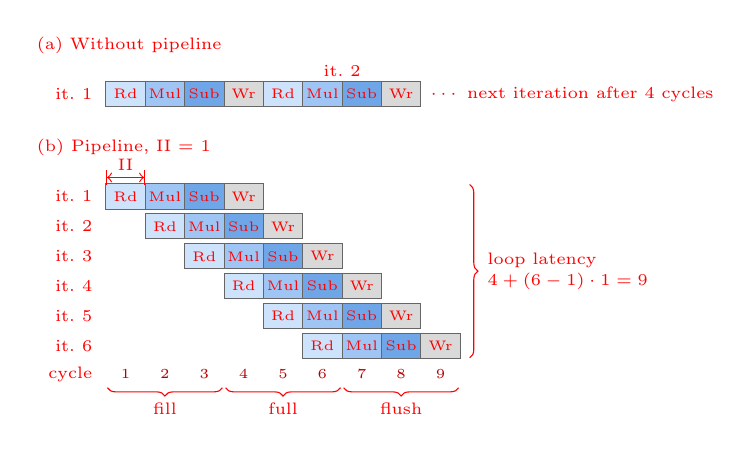
\begin{tikzpicture}[font=\fontsize{6.5}{7.8}\selectfont,
  every node/.append style={text=red},
  est/.style={draw=black!60, fill=#1, minimum width=0.50cm, minimum height=0.32cm, inner sep=0pt, line width=0.3pt},
  est/.default=white]
\def\u{0.50}\def\h{0.38}
\definecolor{e1}{HTML}{CDE2FB}\definecolor{e2}{HTML}{9EC5F4}\definecolor{e3}{HTML}{6FA6E8}\definecolor{e4}{HTML}{D9D9D9}
% estágios de uma iteração: Rd, Mul, Sub, Wr (latência de 4 ciclos)
\newcommand{\iter}[3]{% #1 = ciclo de início (0-index), #2 = linha, #3 = rótulo
  \node[est=e1] at (#1*\u+0.5*\u, -#2*\h) {\fontsize{5}{6}\selectfont Rd};
  \node[est=e2] at (#1*\u+1.5*\u, -#2*\h) {\fontsize{5}{6}\selectfont Mul};
  \node[est=e3] at (#1*\u+2.5*\u, -#2*\h) {\fontsize{5}{6}\selectfont Sub};
  \node[est=e4] at (#1*\u+3.5*\u, -#2*\h) {\fontsize{5}{6}\selectfont Wr};
  \node[left] at (-0.05, -#2*\h) {#3};}
% (a) sem pipeline
\node[anchor=west] at (-1.0, 0.62) {(a) Without pipeline};
\iter{0}{0}{it.~1}
\begin{scope}[shift={(4*\u,0)}]
  \node[est=e1] at (0.5*\u,0) {\fontsize{5}{6}\selectfont Rd};
  \node[est=e2] at (1.5*\u,0) {\fontsize{5}{6}\selectfont Mul};
  \node[est=e3] at (2.5*\u,0) {\fontsize{5}{6}\selectfont Sub};
  \node[est=e4] at (3.5*\u,0) {\fontsize{5}{6}\selectfont Wr};
\end{scope}
\node at (6*\u, 0.30) {it.~2};
\node[right] at (8*\u, 0) {$\cdots$ next iteration after 4 cycles};
% (b) com pipeline, II = 1, 6 iterações
\begin{scope}[shift={(0,-1.30)}]
\node[anchor=west] at (-1.0, 0.62) {(b) Pipeline, II = 1};
\foreach \i in {0,...,5} { \pgfmathtruncatemacro{\r}{\i+1} \iter{\i}{\i}{it.~\r} }
% eixo dos ciclos
\foreach \c in {1,...,9} \node[text=red!70!black] at (\c*\u-0.5*\u, -6*\h+0.02) {\fontsize{5}{6}\selectfont\c};
\node[left] at (-0.05, -6*\h+0.02) {cycle};
% II
\draw[red, |<->|, line width=0.4pt] (0,0.24) -- (\u,0.24) node[midway, above=-1pt] {II};
% enchimento, regime e esvaziamento
\draw[decorate, decoration={brace, mirror, amplitude=3pt}, red, line width=0.4pt] (0.02,-6*\h-0.15) -- (3*\u-0.02,-6*\h-0.15) node[midway, below=2pt, align=center] {fill};
\draw[decorate, decoration={brace, mirror, amplitude=3pt}, red, line width=0.4pt] (3*\u+0.02,-6*\h-0.15) -- (6*\u-0.02,-6*\h-0.15) node[midway, below=2pt, align=center] {full};
\draw[decorate, decoration={brace, mirror, amplitude=3pt}, red, line width=0.4pt] (6*\u+0.02,-6*\h-0.15) -- (9*\u-0.02,-6*\h-0.15) node[midway, below=2pt, align=center] {flush};
\draw[decorate, decoration={brace, amplitude=3pt}, red, line width=0.4pt] (9*\u+0.12,0.15) -- (9*\u+0.12,-5*\h-0.15) node[midway, right=3pt, align=left] {loop latency\\$4 + (6-1)\cdot 1 = 9$};
\end{scope}
\end{tikzpicture}
\end{minipage}
\vspace{4pt}
\legend{\textcolor{red}{Source: the author. Rd: read, Mul: multiply, Sub: subtract, Wr: write. Iteration latency of 4 cycles, as in the example of the book \cite[p.~45]{kastner-hls}.}}
\end{figure}

% ---------------------------------------------------------------------
\subsubsection{\texorpdfstring{\textcolor{red}{Dataflow entre etapas}}{Dataflow entre etapas}}\label{subsubsec:hw-dataflow}

\textcolor{red}{A arquitetura 4545 mantém o \textit{pipeline} dos laços e junta as funções do módulo em quatro etapas. A primeira é a decomposição LU. A segunda calcula a matriz $\mathbf F$ (\texttt{D\_extraction}, \texttt{D\_square\_root} e \texttt{G\_decomposition}). A terceira é a substituição direta, e a quarta, a inversão. A diretiva \texttt{\#pragma HLS dataflow}, na função de topo, transforma cada etapa em um processo. Assim, uma matriz nova entra na primeira etapa assim que a matriz anterior passa para a segunda \cite[p.~114]{kastner-hls}.}
% FONTE: cholesky_hardware_diretivas_4545/cholesky_top.cpp (etapa_lu, etapa_g, etapa_fs,
%   etapa_inv; dataflow em cholesky_inverse, linha 68).

\textcolor{red}{O \textit{dataflow} forma um \textit{pipeline} de tarefas, controlado pela troca de sinais entre os processos. O \textit{pipeline} de laços, por sua vez, age ciclo a ciclo \cite[pp.~114--115]{kastner-hls}. Entre dois processos, os dados passam por uma FIFO ou por um \textit{buffer} ping-pong. O \textit{buffer} ping-pong tem dois blocos: o processo que produz os dados escreve em um, enquanto o processo que os consome lê o outro \cite[p.~115]{kastner-hls}.}

\textcolor{red}{Cada etapa leva a diretiva \texttt{\#pragma HLS inline off}. Essa diretiva impede o HLS de copiar a função para dentro da função que a chama, e mantém a hierarquia do código \cite[p.~52]{kastner-hls}. Assim, cada etapa continua sendo uma função separada e vira um processo.}

\textcolor{red}{Na Figura~\ref{fig:hw-dataflow}, a latência de uma matriz é a soma das quatro etapas. Uma etapa só recebe a matriz seguinte depois de terminar a anterior. Por isso, o intervalo é a duração da etapa mais longa. Sem \textit{dataflow}, a matriz 2 só começaria no fim da matriz 1.}
% SEM FONTE: "intervalo = etapa mais longa" é lido da figura (não achei frase no Kastner;
%   a p. 97 fala de "weakest link", mas de uma porta de memória).

\begin{figure}[!ht]
\caption{\textcolor{red}{Dataflow between the stages of the inversion. The code is simplified, and the durations are not to scale.}}
\label{fig:hw-dataflow}
\vspace{4pt}
\centering
\begin{minipage}[c]{0.33\textwidth}
\color{red}\fontsize{7}{8.6}\selectfont
\begin{verbatim}
void cholesky_inverse(A, inverse) {
#pragma HLS dataflow
  etapa_lu(A, L, U);
  etapa_g(U, L, G);
  etapa_fs(G, G_inv);
  etapa_inv(G_inv, inverse);
}

static void etapa_fs(G, G_inv) {
#pragma HLS inline off
  forward_substitution(G, G_inv);
}
\end{verbatim}
\end{minipage}\hfill
\begin{minipage}[c]{0.64\textwidth}
\centering
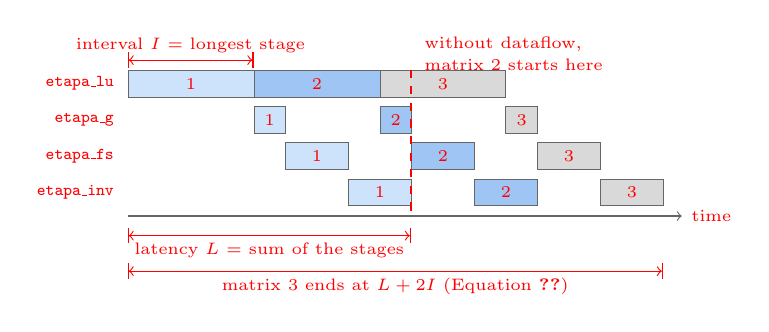
\begin{tikzpicture}[font=\fontsize{6.5}{7.8}\selectfont,
  every node/.append style={text=red},
  tar/.style={draw=black!60, fill=#1, minimum height=0.34cm, inner sep=0pt, line width=0.3pt}]
\def\u{0.40}\def\h{0.46}
\definecolor{m1}{HTML}{CDE2FB}\definecolor{m2}{HTML}{9EC5F4}\definecolor{m3}{HTML}{D9D9D9}
% durações esquemáticas: LU = 4, G = 1, FS = 2, INV = 2 (soma 9, maior 4)
\newcommand{\caixa}[5]{% #1 linha, #2 início, #3 duração, #4 cor, #5 matriz
  \node[tar=#4, minimum width=#3*\u cm, anchor=west] at (#2*\u, -#1*\h) {#5};}
\foreach \l/\n in {0/etapa\_lu, 1/etapa\_g, 2/etapa\_fs, 3/etapa\_inv}
  \node[left, font=\fontsize{6.2}{7.4}\selectfont\ttfamily] at (-0.05, -\l*\h) {\n};
% matriz 1
\caixa{0}{0}{4}{m1}{1}\caixa{1}{4}{1}{m1}{1}\caixa{2}{5}{2}{m1}{1}\caixa{3}{7}{2}{m1}{1}
% matriz 2
\caixa{0}{4}{4}{m2}{2}\caixa{1}{8}{1}{m2}{2}\caixa{2}{9}{2}{m2}{2}\caixa{3}{11}{2}{m2}{2}
% matriz 3
\caixa{0}{8}{4}{m3}{3}\caixa{1}{12}{1}{m3}{3}\caixa{2}{13}{2}{m3}{3}\caixa{3}{15}{2}{m3}{3}
% eixo
\draw[black!60, ->, line width=0.4pt] (0,-3*\h-0.3) -- (17.6*\u,-3*\h-0.3) node[right] {time};
% intervalo
\draw[red, |<->|, line width=0.4pt] (0,0.30) -- (4*\u,0.30) node[midway, above=-1pt] {interval $I$ = longest stage};
% latência da matriz 1
\draw[red, |<->|, line width=0.4pt] (0,-3*\h-0.55) -- (9*\u,-3*\h-0.55) node[midway, below=-1pt] {latency $L$ = sum of the stages};
% sem dataflow
\draw[red, dashed, line width=0.4pt] (9*\u,0.18) -- (9*\u,-3*\h-0.3);
\node[align=left, anchor=south west] at (9*\u+0.05,0.05) {without dataflow,\\matrix 2 starts here};
% fim da matriz 3
\draw[red, |<->|, line width=0.4pt] (0,-3*\h-1.0) -- (17*\u,-3*\h-1.0) node[midway, below=-1pt] {matrix 3 ends at $L + 2I$ (Equation~\ref{eq:fim-tarefas})};
\end{tikzpicture}
\end{minipage}
\vspace{4pt}
\legend{\textcolor{red}{Source: the author. Numbers in the boxes: index of the matrix.}}
\end{figure}

% ---------------------------------------------------------------------
\subsubsection{\texorpdfstring{\textcolor{red}{Lotes de matrizes em vias}}{Lotes de matrizes em vias}}\label{subsubsec:hw-lotes}

\textcolor{red}{Nas arquiteturas 606 e 455, o módulo recebe várias matrizes $\mathbf G_c$ de uma vez, cada uma de um PRB. Esse conjunto é um lote. O lote tem 12 matrizes na 606 e 16 na 455. As matrizes de um lote não dependem umas das outras. As etapas do lote formam um \textit{dataflow}, como na 4545, e um lote novo entra a cada intervalo de lote. O intervalo por matriz é o intervalo do lote dividido pelo número de matrizes do lote, e é ele que deve atender o limite da Tabela~\ref{tab:limite-ciclos}. O número de lotes de um bloco é $N_{\text{PRB}}$ dividido pelo tamanho do lote, arredondado para cima. O último lote vai incompleto. Na Equação~\eqref{eq:fim-tarefas}, a tarefa passa a ser o lote.}
% FONTE: cholesky_hardware_diretivas_606/cholesky_top.cpp (comentário do topo; LOTE e
%   VIAS em cholesky.h; dataflow na linha 315 com lote_ler, lote_lu, lote_g, lote_fs,
%   lote_inv, lote_gravar). LOTE/VIAS: 12/6 (606), 16/8 (455).

\textcolor{red}{As matrizes do lote ficam em bancos de memória separados, com a diretiva \texttt{\#pragma HLS array\_partition cyclic} no índice da matriz. A partição cíclica distribui os elementos entre os bancos de forma alternada. Por exemplo, com fator 2, o vetor 1, 2, \ldots, 9 vira os vetores 1, 3, 5, 7, 9 e 2, 4, 6, 8 \cite[p.~88]{kastner-hls}. Com fator igual ao número de vias, a matriz $m$ fica no banco $m \bmod \text{vias}$. Uma via é o conjunto de operadores que trata um banco. A 606 tem 6 vias, e a 455, 8.}

\textcolor{red}{A Figura~\ref{fig:hw-lotes} mostra a 606. Em cada ciclo, o laço com \textit{pipeline} faz a mesma conta em 6 matrizes, uma em cada via. O lote é tratado em grupos de 6 matrizes, que se alternam a cada ciclo. Como as matrizes não dependem umas das outras, uma iteração não espera o resultado da anterior. As divisões também alternam entre as matrizes do lote, uma por ciclo. Assim, o divisor, que tem \textit{pipeline}, não espera o resultado da divisão anterior.}

\begin{figure}[!ht]
\caption{\textcolor{red}{Batch of 12 matrices in 6 lanes, in the 606 architecture. The code is simplified.}}
\label{fig:hw-lotes}
\vspace{4pt}
\centering
\begin{minipage}[c]{0.43\textwidth}
\color{red}\fontsize{7}{8.6}\selectfont
\begin{verbatim}
#pragma HLS array_partition variable=U \
                     cyclic factor=VIAS dim=1
for (k = column; k < n; k++)
  for (g = 0; g < GRUPOS; g++) {
#pragma HLS pipeline II=1
    for (p = 0; p < VIAS; p++) {
      m = g * VIAS + p;
      t = L[m][line][column] * U[m][column][k];
      U[m][line][k] = U[m][line][k] - t;
    }
  }
\end{verbatim}
\end{minipage}\hfill
\begin{minipage}[c]{0.54\textwidth}
\centering
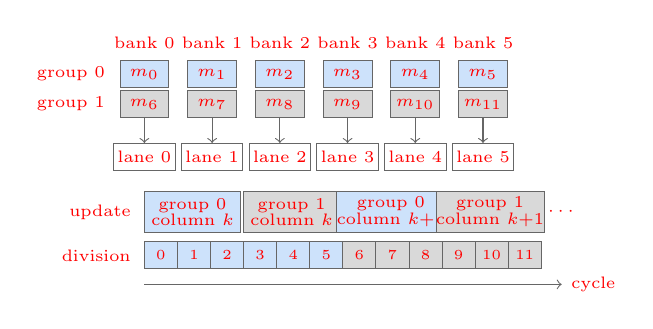
\begin{tikzpicture}[font=\fontsize{6.5}{7.8}\selectfont,
  every node/.append style={text=red},
  mat/.style={draw=black!60, fill=#1, minimum width=0.62cm, minimum height=0.34cm, inner sep=0pt, line width=0.3pt},
  via/.style={draw=black!60, fill=white, minimum width=0.78cm, minimum height=0.34cm, inner sep=0pt, line width=0.3pt}]
\def\u{0.86}
\definecolor{g0}{HTML}{CDE2FB}\definecolor{g1}{HTML}{D9D9D9}
% bancos: matriz m no banco m mod 6
\foreach \p in {0,...,5} {
  \pgfmathtruncatemacro{\q}{\p+6}
  \node at (\p*\u, 0.40) {bank \p};
  \node[mat=g0] at (\p*\u, 0) {$m_{\p}$};
  \node[mat=g1] at (\p*\u, -0.38) {$m_{\q}$};
  \node[via] (v\p) at (\p*\u, -1.05) {lane \p};
  \draw[black!60, ->, line width=0.4pt] (\p*\u, -0.56) -- (v\p.north);
}
\node[left] at (-0.38, 0) {group 0};
\node[left] at (-0.38, -0.38) {group 1};
% ciclos do laço de atualização
\begin{scope}[shift={(0,-1.75)}]
\foreach \c/\g/\k/\cor in {0/0/k/g0, 1/1/k/g1, 2/0/k{+}1/g0, 3/1/k{+}1/g1} {
  \node[mat=\cor, minimum width=1.22cm, minimum height=0.52cm, align=center, font=\fontsize{6}{7}\selectfont] at (\c*1.26+0.61, 0) {group \g\\[-1pt]column $\k$};
}
\node[left] at (-0.05, 0) {update};
\node[right] at (5.0, 0) {$\cdots$};
\foreach \c in {0,...,11} {
  \pgfmathtruncatemacro{\gg}{\c<6 ? 0 : 1}
  \ifnum\gg=0 \def\cc{g0}\else\def\cc{g1}\fi
  \node[mat=\cc, minimum width=0.42cm] at (\c*0.42+0.21, -0.55) {\fontsize{5.5}{6}\selectfont\c};
}
\node[left] at (-0.05, -0.55) {division};
\draw[black!60, ->, line width=0.4pt] (0,-0.92) -- (5.3,-0.92) node[right] {cycle};
\end{scope}
\end{tikzpicture}
\end{minipage}
\vspace{4pt}
\legend{\textcolor{red}{Source: the author. Update: one cycle per box, 6 matrices at a time. Division: one matrix per cycle, in a single divider; the numbers are the indices $m$ of the matrices.}}
\end{figure}

% ---------------------------------------------------------------------
\subsubsection{\texorpdfstring{\textcolor{red}{Arranjo sistólico}}{Arranjo sistólico}}\label{subsubsec:hw-sistolico}

\textcolor{red}{As arquiteturas 152 e 114 também usam lotes, com 32 matrizes. A 152 tem 2 vias, e a 114 tem 4. Cada via tem o seu próprio divisor. Além disso, o laço que percorre uma linha ou uma soma é desenrolado em células, uma para cada índice $k$, lado a lado. Cada célula só troca dados com a vizinha. Projetos assim são chamados de arranjos sistólicos, e podem surgir quando um laço interno é desenrolado \cite[p.~180]{kastner-hls}.}
% FONTE: cholesky_hardware_diretivas_152_sistolico/cholesky_top.cpp (comentário do topo);
%   LOTE/VIAS: 32/2 (152), 32/4 (114).

\textcolor{red}{Na substituição direta e na inversão, a soma parcial passa de uma célula para a seguinte, na mesma ordem de somas da versão sem otimizações. Assim, cada ciclo calcula uma soma inteira. Na decomposição LU, cada célula atualiza um elemento da linha, e cada ciclo atualiza uma linha inteira. Para as células lerem todos os índices $k$ no mesmo ciclo, cada elemento da linha fica em um banco próprio, com \texttt{\#pragma HLS array\_partition complete} \cite[p.~41]{kastner-hls}.}

\textcolor{red}{Na decomposição LU e na substituição direta, cada passo usa as linhas gravadas no passo anterior. As matrizes do lote se alternam a cada ciclo. Assim, entre a gravação de uma linha e a sua leitura, passam tantos ciclos quanto o tamanho do passo. Os passos curtos recebem ciclos vazios, até um número mínimo de ciclos. Com isso, uma linha só é lida depois de sair do \textit{pipeline}. A diretiva \texttt{\#pragma HLS dependence ... dependent=false} informa isso ao HLS. Essa diretiva passa ao HLS uma informação que ele não consegue deduzir do código, e cabe ao projetista garantir que ela é verdadeira \cite[pp.~149--150]{kastner-hls}. Se o \textit{pipeline} ficar mais profundo que o passo, o resultado fica errado. A simulação da netlist, que compara as inversas com as do código C (Seção~\ref{subsec:hw-potencia}), confere isso. A Figura~\ref{fig:hw-sistolico} mostra as células e os ciclos vazios.}
% FONTE: comentário do topo de cholesky_top.cpp da 152 (CHOL_PROF_LU, CHOL_PROF_FS;
%   lu_passo, fs_passo; "Se a profundidade real do pipeline passar de CHOL_PROF_*, o
%   resultado do RTL fica errado; a co-simulação confere isso").

\begin{figure}[!ht]
\caption{\textcolor{red}{Systolic array of the forward substitution and minimum step of the LU decomposition. The code is simplified.}}
\label{fig:hw-sistolico}
\vspace{4pt}
\centering
\begin{minipage}[c]{0.42\textwidth}
\color{red}\fontsize{7}{8.6}\selectfont
\begin{verbatim}
#pragma HLS array_partition variable=Ua \
                     complete dim=3
for (it = 0; it < LU_ITER; it++) {
#pragma HLS pipeline II=1
#pragma HLS dependence variable=Ua \
          type=inter dependent=false
  if (idx < reais)       // else: empty
    for (p = 0; p < VIAS; p++)
      for (k = 0; k < n; k++)  // cells
        Ua[m][line][k] = row[k] - l*piv[k];
}
\end{verbatim}
\end{minipage}\hfill
\begin{minipage}[c]{0.55\textwidth}
\centering
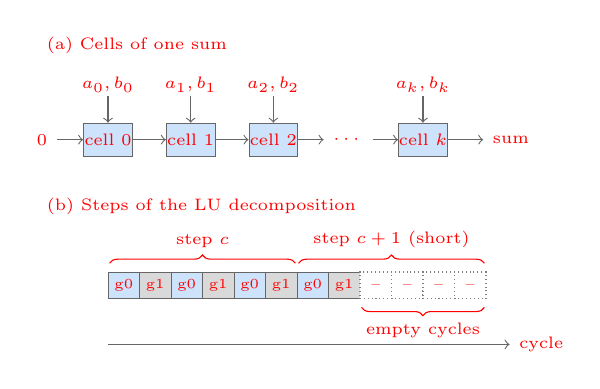
\begin{tikzpicture}[font=\fontsize{6.5}{7.8}\selectfont,
  every node/.append style={text=red},
  cel/.style={draw=black!60, fill=#1, minimum width=0.62cm, minimum height=0.42cm, inner sep=0pt, line width=0.3pt},
  cel/.default={white},
  seta/.style={black!60, ->, line width=0.4pt}]
\definecolor{c0}{HTML}{CDE2FB}\definecolor{c1}{HTML}{D9D9D9}
% (a) células em cadeia: s_k = s_{k-1} + a_k b_k
\node[anchor=west] at (-0.9, 1.20) {(a) Cells of one sum};
\foreach \k/\x/\l in {0/0/0, 1/1.05/1, 2/2.10/2} {
  \node[cel=c0] (c\k) at (\x, 0) {cell \l};
  \draw[seta] (\x, 0.55) node[above=-2pt] {$a_{\l}, b_{\l}$} -- (c\k.north);
}
\node (dots) at (3.05, 0) {$\cdots$};
\node[cel=c0] (cn) at (4.0, 0) {cell $k$};
\draw[seta] (4.0, 0.55) node[above=-2pt] {$a_{k}, b_{k}$} -- (cn.north);
\draw[seta] (-0.65, 0) node[left] {$0$} -- (c0.west);
\draw[seta] (c0) -- (c1); \draw[seta] (c1) -- (c2); \draw[seta] (c2) -- (dots); \draw[seta] (dots) -- (cn);
\draw[seta] (cn.east) -- ++(0.45, 0) node[right] {sum};
% (b) passos da LU com ciclos vazios
\begin{scope}[shift={(0,-1.85)}]
\node[anchor=west] at (-0.9, 1.00) {(b) Steps of the LU decomposition};
\def\w{0.40}
\foreach \i/\g in {0/0, 1/1, 2/0, 3/1, 4/0, 5/1} {
  \ifnum\g=0 \def\cc{c0}\else\def\cc{c1}\fi
  \node[cel=\cc, minimum width=0.40cm, minimum height=0.34cm] at (\i*\w+0.5*\w, 0) {\fontsize{5}{6}\selectfont g\g};
}
\foreach \i/\g in {6/0, 7/1} {
  \ifnum\g=0 \def\cc{c0}\else\def\cc{c1}\fi
  \node[cel=\cc, minimum width=0.40cm, minimum height=0.34cm] at (\i*\w+0.5*\w, 0) {\fontsize{5}{6}\selectfont g\g};
}
\foreach \i in {8,...,11}
  \node[draw=black!50, fill=white, densely dotted, minimum width=0.40cm, minimum height=0.34cm, inner sep=0pt, line width=0.4pt] at (\i*\w+0.5*\w, 0) {\fontsize{5}{6}\selectfont --};
\draw[decorate, decoration={brace, amplitude=3pt}, red, line width=0.4pt] (0.02, 0.28) -- (6*\w-0.02, 0.28) node[midway, above=2pt] {step $c$};
\draw[decorate, decoration={brace, amplitude=3pt}, red, line width=0.4pt] (6*\w+0.02, 0.28) -- (12*\w-0.02, 0.28) node[midway, above=2pt] {step $c+1$ (short)};
\draw[decorate, decoration={brace, mirror, amplitude=3pt}, red, line width=0.4pt] (8*\w+0.02, -0.28) -- (12*\w-0.02, -0.28) node[midway, below=2pt] {empty cycles};
\draw[black!60, ->, line width=0.4pt] (0,-0.75) -- (12*\w+0.3,-0.75) node[right] {cycle};
\end{scope}
\end{tikzpicture}
\end{minipage}
\vspace{4pt}
\legend{\textcolor{red}{Source: the author. g0 and g1: groups of matrices of the batch, one per cycle. Two groups are drawn for clarity: the 152 has 16 groups, and the 114 has 8. In (b), the short step is filled with empty cycles up to a minimum length, so that a row is read only after it leaves the pipeline.}}
\end{figure}

% ---------------------------------------------------------------------
\subsection{\texorpdfstring{\textcolor{red}{Test Matrices}}{Test Matrices}}\label{subsec:hw-matrizes}
% ---------------------------------------------------------------------
\textcolor{red}{O hardware foi testado com as matrizes $\mathbf{G}_c$ que o BCD-MMSE inverte no simulador. Um script roda o simulador com a mesma semente e salva cada $\mathbf{G}_c$ antes da inversão. O simulador não muda. Assim, as matrizes são exatamente as usadas nas curvas de SER, com 1 iteração do BCD-MMSE.}
% EN (versão anterior, 2026-11-05): The hardware was tested with the matrices $\mathbf{G}_c$ that the BCD-MMSE inverts in the simulator. A script runs the simulator with the same seed and saves each $\mathbf{G}_c$ before the inversion. The simulator does not change. So the matrices are exactly the ones used for the SER curves, with 1 BCD-MMSE iteration.
% FONTE: AMOSTRAGEM.md, seções 1 e 2 (exportar_matrizes.py troca a função de inversão
%   só na memória do processo; matrizes recalculadas por fora coincidem até 1e-12).

\textcolor{red}{Como as condições de teste só mudam $N$ e a portadora (Seção~\ref{subsec:setup_condicoes}), as matrizes foram exportadas uma vez para cada par da Tabela~\ref{tab:condicoes_teste}. São 5 pares, pois TDLA30-5 e TDLA30-10 têm o mesmo par.}
% ANTIGO (2026-11-05, repetia Test Conditions e a Tabela tab:condicoes_teste):
% \textcolor{red}{As condições de teste mudam só dois valores nessas matrizes: o número de amostras de ruído $N$ e a frequência de portadora. Condições com o mesmo $N$ e a mesma portadora dão as mesmas matrizes. Por isso, as matrizes foram exportadas uma vez para cada par: 192 amostras a 3,5~GHz (TDLA30-5 e TDLA30-10), 192 a 28~GHz (TDLA30-75), 168 a 28~GHz (TDLA30-300), 132 a 3,5~GHz (TDLC300-100) e 24 a 3,5~GHz (TDLB100-400).}
% EN (versão anterior, 2026-11-05): The test conditions change only two values in these matrices: the number of noise samples $N$ and the carrier frequency. Test conditions with the same $N$ and the same carrier give the same matrices. So the matrices were exported once for each pair: 192 samples at 3.5~GHz (TDLA30-5 and TDLA30-10), 192 at 28~GHz (TDLA30-75), 168 at 28~GHz (TDLA30-300), 132 at 3.5~GHz (TDLC300-100) and 24 at 3.5~GHz (TDLB100-400).
% FONTE: AMOSTRAGEM.md, tabela das pastas (2_amostra_matrizes/amostras<N>_fc<GHz>GHz).

\textcolor{red}{A modulação não muda $\mathbf{G}_c = E_s\mathbf{H}_c\mathbf{H}_c^H + \hat{\mathbf{R}}_{cc}$. Em cada grupo, as configurações QPSK (C, D, G e H) diferem das configurações 16-QAM (A, B, E e F) só na modulação. Por isso, as configurações QPSK não foram exportadas.}
% ANTIGO (2026-11-06): "As configurações 1C, 1D, 1G e 1H diferem de 1A, 1B, 1E e 1F só na modulação."
%   Citava só o grupo 1, mas as QPSK dos grupos 2 e 3 também não foram exportadas
%   (indice.csv: 16x16 só 1A, 1B, 1E, 1F, 3A, 3B, 3E, 3F; 32x32 só 2A, 2B, 2E, 2F).
% EN (versão anterior, 2026-11-05): The modulation does not change $\mathbf{G}_c = E_s\mathbf{H}_c\mathbf{H}_c^H + \hat{\mathbf{R}}_{cc}$. Configurations 1C, 1D, 1G and 1H differ from 1A, 1B, 1E and 1F only in the modulation. Therefore, the QPSK configurations were not exported.
% FONTE: AMOSTRAGEM.md, seção 4 ("As configurações 5 a 8 ficam fora por padrão").
% CUIDADO: a distribuição de G_c é a mesma para a mesma SNR. No ponto de operação, a
%   SNR do QPSK é menor, e G_c fica maior (tab:gc-ponto-operacao). As matrizes do QPSK
%   aparecem nos pontos de SNR baixa das configurações 16-QAM.

\textcolor{red}{Exportar todas as matrizes não é prático. Para cada par, a amostra tem duas partes. A primeira sorteia 3 matrizes para cada configuração e ponto de SNR, para cobrir os pontos de operação da simulação. A segunda pega as 5 matrizes com os valores mais extremos de quatro métricas: a maior parte real ou imaginária, o maior elemento da inversa, o menor autovalor e o número de condição. Esses são os piores casos de faixa e de precisão para o formato de ponto fixo.}
% EN (versão anterior, 2026-11-05): Exporting every matrix is not practical. For each pair, the sample has two parts. The first part draws 3 matrices for each configuration and SNR point, to cover the operating points of the simulation. The second part takes the 5 matrices with the most extreme values of four metrics: the largest real or imaginary part, the largest element of the inverse, the smallest eigenvalue and the condition number. These are the worst cases of range and precision for the fixed-point format.
% FONTE: AMOSTRAGEM.md, seção 4 (critérios "cobertura" e extremos; semente 0) e seção 5
%   (264 matrizes 16x16 e 132 matrizes 32x32 de cobertura por par, mais até 20 extremos).

% ---------------------------------------------------------------------
\subsection{\texorpdfstring{\textcolor{red}{Power and Energy}}{Power and Energy}}\label{subsec:hw-potencia}
% ---------------------------------------------------------------------
\textcolor{red}{A potência foi estimada com a atividade de chaveamento do projeto roteado. Para cada condição de teste, um testbench inverte 20 matrizes da amostra, uma depois da outra. As 20 matrizes são espalhadas pelas configurações e sorteadas com uma semente fixa: configurações 1A, 1B, 1E e 1F no circuito $16 \times 16$, e 2A, 2B, 2E e 2F no circuito $32 \times 32$. O circuito $16 \times 16$ também atende o grupo 3, mas a sua potência foi estimada só com matrizes do grupo 1. Nas arquiteturas com lote, o testbench inverte lotes inteiros, e são pelo menos 3 lotes, para medir o intervalo entre lotes. As 20 matrizes são repetidas em ordem até completar os lotes. Assim, a 606 inverte 36 matrizes, a 455 inverte 48, e a 152 e a 114 invertem 96.}
% ANTIGO (2026-11-06): o parágrafo terminava em "... 2A, 2B, 2E e 2F no circuito $32 \times 32$."
% FONTE (lotes): tb_potencia.cpp da 606 (linhas 57-71: lotes = max(3, ceil(20/LOTE)); matriz
%   (b*LOTE+m) % 20); coluna "matrizes" de resultados_servidor/**/potencia.csv: 36 (606),
%   48 (455), 96 (152 e 114), 20 nas outras.
% EN (versão anterior, 2026-11-05): The power was estimated with the switching activity of the routed design. For each test condition, a testbench inverts 20 matrices from the sample, one after the other. The 20 matrices are spread over the configurations of the circuit and drawn with a fixed seed: configurations 1A--1H for the $16 \times 16$ circuit, and 2A, 2B, 2E and 2F for the $32 \times 32$ circuit.
% FONTE: rodar_potencia.py (sinteses/*_vivado/potencia/): "20 matrizes ... configurações
%   1 a 8 [16x16] / 9 a 12 [32x32], espalhadas pelas configurações e sorteadas com
%   semente fixa"; tb_potencia.cpp. Nas versões com lote, o testbench inverte lotes
%   inteiros (pelo menos 3), então o número de matrizes pode passar de 20
%   (potencia_versoes.py). CONFERIDO (2026-11-06): ver o FONTE (lotes) acima.
% CORRIGIDO (2026-11-06): o texto dizia "configurações 1A--1H". rodar_potencia.py sorteia
%   das configurações 1 a 8 (numeração antiga), mas as QPSK (5 a 8 = 1C, 1D, 1G, 1H) não
%   foram exportadas: o indice.csv do 16x16 só tem 1-4 (1A, 1E, 1B, 1F) e 13-16 (3A, 3E, 3B,
%   3F). Logo, só 1A, 1B, 1E e 1F entram. O grupo 3 está na amostra, mas não na potência
%   (decisão da autora: não rodar de novo).

\textcolor{red}{O Vivado gera uma netlist funcional do projeto roteado. A netlist é simulada no simulador do Vivado com o testbench, e a atividade de cada sinal é salva em um arquivo SAIF. As inversas calculadas pela netlist são comparadas, byte a byte, com as inversas do código C. Depois, o arquivo SAIF é lido no projeto roteado, e o Vivado informa a potência.}
% EN (versão anterior, 2026-11-05): Vivado writes a functional netlist of the routed design. The netlist is simulated in the Vivado simulator with the testbench, and the activity of every signal is saved in a SAIF file. The inverses computed by the netlist are compared, byte by byte, with the inverses of the C code. Then the SAIF file is read in the routed design, and Vivado reports the power.
% FONTE: potencia.py, passos 1 a 5 (write_verilog -mode funcsim; xsim com -debug typical;
%   read_saif; report_power). TODO FONTE: guia de análise de potência do Vivado (UG907).

\textcolor{red}{A versão sem otimizações foi simulada nas 5 condições de teste. Cada arquitetura otimizada foi simulada só na sua condição de teste alvo. A TDLA30-10 usa as mesmas matrizes da TDLA30-5.}
% EN (versão anterior, 2026-11-05): The version without optimizations was simulated in the 5 test conditions. Each optimized architecture was simulated only in its target test condition. TDLA30-10 uses the same matrices as TDLA30-5.
% FONTE: memória tcc-potencia-cenario-por-versao; pacote_servidor_formatos/LEIAME.md.
%   Justificativa: na versão sem otimização, a potência quase não mudou entre as
%   condições (ex.: 0,047 x 0,046 W no TDLB100-400). Isso é resultado.

\textcolor{red}{A energia por inversão é a potência dinâmica multiplicada pelo tempo entre duas inversões. Esse tempo é o intervalo em regime, em ciclos de clock, medido na simulação da netlist, multiplicado pelo período de 10~ns. Nas arquiteturas com lote, o intervalo medido é o do lote. Ele é dividido pelo número de matrizes do lote, para dar o intervalo por matriz (Seção~\ref{subsubsec:hw-lotes}).}
% ANTIGO (2026-11-06): o parágrafo terminava em "... multiplicado pelo período de 10~ns."
% EN (versão anterior, 2026-11-05): The energy per inversion is the dynamic power multiplied by the time between two inversions. This time is the steady-state interval, in clock cycles, measured in the netlist simulation, multiplied by the 10~ns period.
% FONTE: memória tcc-pacote-servidor-2023 (convenção da energia). Intervalo tirado do
%   xsim_<cenário>.log do servidor, não do ciclos_medios do potencia.csv, que inclui o
%   enchimento do pipeline do primeiro lote.


% =====================================================================
\section{\texorpdfstring{\textcolor{red}{Organização dos resultados}}{Organização dos resultados}}\label{sec:organizacao-resultados}
% =====================================================================


% ---------------------------------------------------------------------
% 1.6  ORGANIZAÇÃO DOS RESULTADOS                 -> fim da Metodologia
% ---------------------------------------------------------------------
\textcolor{red}{Os resultados são agrupados pelas características físicas da estação base: o tamanho do circuito de inversão ($16 \times 16$ ou $32 \times 32$), o número $M$ de antenas e o número $C$ de \textit{clusters}. Dentro de cada grupo, variam a modulação, $K$ e a IoTh. Assim, há três grupos: as configurações 1A--1H ($M = 128$, $C = 8$, circuito $16 \times 16$), 2A--2H ($M = 256$, $C = 8$, circuito $32 \times 32$) e 3A--3H ($M = 256$, $C = 16$, circuito $16 \times 16$).}
% ORIGEM: Análise bits.md, "hard-constraints" (M, C, tamanho do circuito) e
%   "soft-constraints" (modulação, K, IoTh). Os nomes G1-G3 não vão para a tese.


% =====================================================================
\chapter{Resultados}
% =====================================================================

% =====================================================================
% RASCUNHO -- seção "Setup de simulação" reorganizada por módulo do simulador
% ---------------------------------------------------------------------
% Incluído em 9-results.tex por \input{chapters/rascunho_setup_simulacao}.
% Substitui o setup antigo (cópia em rascunho_setup_antigo.tex) e
% rascunho_setup_tabelas.tex (as tabelas estão copiadas aqui).
% A entrada tomasin-interference precisa ir para o biblio.bib.
%
% Marcas:
%   % AUTORA (9-results.tex:NNN)  -> texto seu, sem alteração, só mudou de lugar
%   % NOVO                        -> texto proposto; cada frase tem FONTE ou SEM FONTE
%
% Chaves de citação: zhao2025jsac (já existe); tomasin-interference (em
% constraints/rascunho_referencias.bib). ATENÇÃO: rascunho_bloco_canal.tex
% usa a chave antiga zhao-lmmse; trocar por zhao2025jsac se for aproveitado.
% "Lnnn" = linha do paper.md do artigo base.
% =====================================================================

\section{Setup de simulação}

% NOVO -- substitui 9-results.tex:4
Os parâmetros da simulação estão organizados de acordo com a parte do simulador em que são usados: o canal, o sinal e o ruído, o receptor e a avaliação. Os parâmetros do sistema seguem o modelo de \citeonline{zhao2025jsac}, que propõe os equalizadores descentralizados avaliados neste trabalho. Em cada tabela, a coluna de origem indica a referência de cada valor.
% TOM: Zhao et al. é a referência do modelo, não objeto de reprodução.


% ---------------------------------------------------------------------
\subsection{Configurações simuladas}
% ---------------------------------------------------------------------
% Vem primeiro: M, C, K, r, IoT e modulação mudam entre as configurações e
% não se repetem nas tabelas seguintes.

% AUTORA (9-results.tex:214), tom ajustado
Foram simuladas seis configurações, as mesmas avaliadas por \citeonline{zhao2025jsac}. A configuração 1 é a de referência. Cada uma das outras muda um parâmetro em relação a ela. A Tabela~\ref{tab:paineis} mostra essas configurações.

\begin{table}[htbp]
\color{red}
\caption{Configurações simuladas.}
\label{tab:paineis}
\centering
\footnotesize
\renewcommand{\arraystretch}{1.2}
\begin{tabular}{|c|c|c|c|c|c|c|}
\hline
Configuração & $M$ & $C$ & $M_c$ & $K$ & IoT (dB) & Modulação \\
\hline
-- & \texttt{M} & \texttt{C} & -- & \texttt{K} & \texttt{iot\_db} & \texttt{modulation} \\
\hline
1 & 128 & 8  & 16 & 8  & 10 & 16-QAM \\
\hline
2 & 256 & 8  & 32 & 8  & 10 & 16-QAM \\
\hline
3 & 256 & 16 & 16 & 8  & 10 & 16-QAM \\
\hline
4 & 128 & 8  & 16 & 12 & 10 & 16-QAM \\
\hline
5 & 128 & 8  & 16 & 8  & 20 & 16-QAM \\
\hline
6 & 128 & 8  & 16 & 8  & 10 & QPSK \\
\hline
\end{tabular}
\legend{\textcolor{red}{Fonte: adaptado de \citeonline{zhao2025jsac}. Em todas as configurações, $r = 8$. Nomes no código: campos de \texttt{Panel} (\texttt{dbp\_sim/params.py}); $M_c = M/C$.}}
\end{table}

% AUTORA (9-results.tex:245) -- parágrafo retirado do texto (tom); o conteúdo ficou em comentário.
% Configurações 1 a 6 = painéis (a), (b), (c), (e), (f), (g) da Fig. 8 de Zhao et al.
% O painel (d) não aparece no artigo. Na configuração 4 (painel e), r = 8 foi
% mantido; L577 liga r a K, então r = 12 também seria defensável.


% ---------------------------------------------------------------------
\subsection{Canal}\label{subsec:setup_canal}
% ---------------------------------------------------------------------

% NOVO
A Tabela~\ref{tab:param_canal} mostra os parâmetros usados para gerar as matrizes de canal $\mathbf{H}$ e $\overline{\mathbf{H}}$.
% AUTORA (9-results.tex:67), adaptado: "A Tabela ... lista esses valores" saiu,
% porque agora os padrões estão na mesma tabela.
Os demais parâmetros do QuaDRiGa foram mantidos no valor padrão do simulador \cite{quadriga-manual}.
% Saiu "e não mudam o resultado de forma importante" (não foi medido).

\begin{table}[htbp]
\caption{Parâmetros do cenário e do canal.}
\label{tab:param_canal}
\centering
\footnotesize
\renewcommand{\arraystretch}{1.0} % 1.0 (e não 1.2) para a legenda caber na página
\begin{tabular}{|p{2.2cm}|p{3.6cm}|p{4.6cm}|p{3.4cm}|}
\hline
\raggedright Origem & \raggedright Parâmetro & \raggedright Nome no código & \raggedright Valor \tabularnewline
\hline
\raggedright \cite{zhao2025jsac} & \raggedright Número de células e de BSs & \raggedright \texttt{M2\_\allowbreak{}Channel.\allowbreak n\_\allowbreak{}cells} & \raggedright 1 \tabularnewline
\cline{2-4}
 & \raggedright Setor onde ficam os UEs & \raggedright \texttt{M2\_\allowbreak{}Channel.\allowbreak sector\_\allowbreak{}deg} & \raggedright $120^\circ$ \tabularnewline
\cline{2-4}
 & \raggedright Distância dos UEs até a BS & \raggedright \texttt{M2\_\allowbreak{}Channel.\allowbreak radius\_\allowbreak{}min\_\allowbreak{}m}, \texttt{radius\_\allowbreak{}max\_\allowbreak{}m} & \raggedright 50 a 100 m \tabularnewline
\cline{2-4}
 & \raggedright Posição dos interferentes & \raggedright \texttt{M2\_\allowbreak{}Channel.\allowbreak interferers\_\allowbreak{}like\_\allowbreak{}targets} & \raggedright Mesma regra dos UEs atendidos \tabularnewline
\cline{2-4}
 & \raggedright Gerador do canal & \raggedright -- & \raggedright QuaDRiGa \tabularnewline
\cline{2-4}
 & \raggedright Canal constante dentro de um PRB & \raggedright -- & \raggedright Canal plano \tabularnewline
\hline
\raggedright Padrão do QuaDRiGa \cite{quadriga-manual} & \raggedright Usa só a versão mínima do modelo 3GPP & \raggedright \texttt{qd\_\allowbreak{}simulation\_\allowbreak{}parameters.\allowbreak use\_\allowbreak{}3GPP\_\allowbreak{}baseline} & \raggedright \texttt{false} \tabularnewline
\cline{2-4}
 & \raggedright Forma da correlação espacial dos parâmetros de larga escala & \raggedright \texttt{qd\_\allowbreak{}simulation\_\allowbreak{}parameters.\allowbreak autocorrelation\_\allowbreak{}function} & \raggedright \texttt{Comb300} \tabularnewline
\cline{2-4}
 & \raggedright Soma o atraso do caminho direto aos atrasos & \raggedright \texttt{qd\_\allowbreak{}simulation\_\allowbreak{}parameters.\allowbreak use\_\allowbreak{}absolute\_\allowbreak{}delays} & \raggedright \texttt{false} \tabularnewline
\cline{2-4}
 & \raggedright Cada caminho começa com uma fase aleatória & \raggedright \texttt{qd\_\allowbreak{}simulation\_\allowbreak{}parameters.\allowbreak use\_\allowbreak{}random\_\allowbreak{}initial\_\allowbreak{}phase} & \raggedright \texttt{true} \tabularnewline
\cline{2-4}
 & \raggedright Amostras por meio comprimento de onda na trajetória & \raggedright \texttt{qd\_\allowbreak{}simulation\_\allowbreak{}parameters.\allowbreak sample\_\allowbreak{}density} & \raggedright 2,5 \tabularnewline
\cline{2-4}
 & \raggedright Altura da BS & \raggedright \texttt{qd\_\allowbreak{}layout.\allowbreak tx\_\allowbreak{}position} & \raggedright 25 m \tabularnewline
\hline
\raggedright Este trabalho & \raggedright Forma de uso do QuaDRiGa & \raggedright \texttt{M2\_\allowbreak{}Channel.\allowbreak backend} & \raggedright Canais exportados em arquivo e lidos em Python \tabularnewline
\cline{2-4}
 & \raggedright Versão do QuaDRiGa & \raggedright \texttt{M2\_\allowbreak{}Channel.\allowbreak quadriga\_\allowbreak{}version} & \raggedright 2.8.1-0 \tabularnewline
\cline{2-4}
 & \raggedright Cenário & \raggedright \texttt{M2\_\allowbreak{}Channel.\allowbreak quadriga\_\allowbreak{}scenario} & \raggedright \texttt{3GPP\_\allowbreak{}38.901\_\allowbreak{}UMa\_\allowbreak{}NLOS} \tabularnewline
\cline{2-4}
 & \raggedright Frequência da portadora & \raggedright \texttt{M2\_\allowbreak{}Channel.\allowbreak center\_\allowbreak{}frequency\_\allowbreak{}hz} & \raggedright 3,5 GHz \tabularnewline
\cline{2-4}
 & \raggedright Largura de banda & \raggedright \texttt{M2\_\allowbreak{}Channel.\allowbreak bandwidth\_\allowbreak{}hz} & \raggedright 20 MHz \tabularnewline
\cline{2-4}
 & \raggedright Extração do canal plano & \raggedright \texttt{M2\_\allowbreak{}Channel.\allowbreak flat\_\allowbreak{}channel\_\allowbreak{}extraction} & \raggedright Resposta em uma subportadora \tabularnewline
\cline{2-4}
 & \raggedright Arranjo da BS & \raggedright \texttt{M2\_\allowbreak{}Channel.\allowbreak array\_\allowbreak{}geometry} & \raggedright ULA com espaçamento $\lambda/2$ \tabularnewline
\cline{2-4}
 & \raggedright Elementos de antena (BS e UE) & \raggedright \texttt{M2\_\allowbreak{}Channel.\allowbreak array\_\allowbreak{}geometry} & \raggedright Omnidirecionais \tabularnewline
\cline{2-4}
 & \raggedright Orientação do setor & \raggedright \texttt{M2\_\allowbreak{}Channel.\allowbreak array\_\allowbreak{}geometry} & \raggedright Centrado na direção perpendicular ao arranjo \tabularnewline
\cline{2-4}
 & \raggedright Altura do UE & \raggedright \texttt{M2\_\allowbreak{}Channel.\allowbreak ue\_\allowbreak{}height\_\allowbreak{}m} & \raggedright 1,5 m \tabularnewline
\cline{2-4}
 & \raggedright Posição dos UEs & \raggedright \texttt{M2\_\allowbreak{}Channel.\allowbreak ue\_\allowbreak{}placement} & \raggedright Uniforme na área do setor \tabularnewline
\cline{2-4}
 & \raggedright Realizações & \raggedright \texttt{M2\_\allowbreak{}Channel.\allowbreak independent\_\allowbreak{}drops} & \raggedright Posições novas a cada realização \tabularnewline
\cline{2-4}
 & \raggedright Normalização do canal & \raggedright \texttt{M2\_\allowbreak{}Channel.\allowbreak normalization} & \raggedright Controle de potência por UE \tabularnewline
\hline
\end{tabular}
\legend{Fonte: \citeonline{zhao2025jsac}, código-fonte do QuaDRiGa v2.8.1 e a autora. $M$, $K$ e $r$ estão na Tabela~\ref{tab:paineis}. Nomes no código: \texttt{dbp\_sim/params.py} e propriedades das classes do QuaDRiGa.} % TODO citar QuaDRiGa
\end{table}
% FONTES (artigo): L577 (célula única, setor, raio, QuaDRiGa, interferentes
%   "molded similarly"); L614 (canal constante no PRB).
% Altura do UE: o script fixa 1,5 m, igual ao padrão de randomize_rx_positions;
%   por isso está em "Escolhido" e não em "Padrão do QuaDRiGa".
% Altura da BS: o script também fixa 25 m, igual ao padrão de qd_layout.
%   Mantida em "Padrão" porque a escolha do cenário se apoia nesse padrão.
%   Se preferir coerência com a altura do UE, mover para "Escolhido".

% AUTORA (9-results.tex:173-175) -- antes na subseção "Cenário escolhido".
% A frase da linha 171 ("O QuaDRiGa define cada cenário por um arquivo de
% configuração...") saiu: o mesmo conceito já está na fundamentação
% (0.channel-modelling.tex, "Cenário de propagação").
Neste trabalho foi usado o cenário \texttt{3GPP\_38.901\_UMa\_NLOS}, que representa uma macrocélula urbana (\textit{Urban Macro} -- UMa) sem linha de visada (NLoS) entre a BS e os UEs. % TODO citar 3GPP TR 38.901 e QuaDRiGa
Os cenários UMa e UMi (\textit{Urban Micro}) aceitam a mesma faixa de distâncias, de 10 a 5000 m. Então o raio de 50 a 100 m não separa os dois. A diferença está na altura da BS: 10 m no UMi e 25 m no UMa. Foi usada a altura padrão do QuaDRiGa, de 25 m, que corresponde ao cenário UMa. % TODO citar QuaDRiGa (qd_layout: tx em [0;0;25])
A Tabela~\ref{tab:cenario_uma} compara a faixa de validade do cenário com os valores usados na simulação.

% AUTORA (9-results.tex:178-209) -- tabela de validade do cenário
\begin{table}[htbp]
\color{red}
\caption{Faixa de validade do cenário \texttt{3GPP\_38.901\_UMa\_NLOS} e valores usados na simulação.}
\label{tab:cenario_uma}
\centering
\footnotesize
\renewcommand{\arraystretch}{1.2}
\begin{tabular}{|p{3.2cm}|p{4.6cm}|p{3.1cm}|p{2.3cm}|}
\hline
\raggedright Parâmetro & \raggedright Nome no código & \raggedright Faixa válida do cenário & \raggedright Valor usado \tabularnewline
\hline
\raggedright Frequência da portadora & \raggedright \texttt{M2\_\allowbreak{}Channel.\allowbreak center\_\allowbreak{}frequency\_\allowbreak{}hz} & \raggedright 0,5 a 100 GHz & \raggedright 3,5 GHz \tabularnewline
\hline
\raggedright Distância BS--UE & \raggedright \texttt{M2\_\allowbreak{}Channel.\allowbreak radius\_\allowbreak{}min\_\allowbreak{}m}, \texttt{radius\_\allowbreak{}max\_\allowbreak{}m} & \raggedright 10 a 5000 m & \raggedright 50 a 100 m \tabularnewline
\hline
\raggedright Altura da BS & \raggedright \texttt{M2\_\allowbreak{}Channel.\allowbreak bs\_\allowbreak{}height\_\allowbreak{}m} & \raggedright 25 m & \raggedright 25 m \tabularnewline
\hline
\raggedright Altura do UE & \raggedright \texttt{M2\_\allowbreak{}Channel.\allowbreak ue\_\allowbreak{}height\_\allowbreak{}m} & \raggedright 1,5 a 22,5 m & \raggedright 1,5 m \tabularnewline
\hline
\raggedright Número de \textit{clusters} & \raggedright \texttt{NumClusters} & \multicolumn{2}{c|}{21} \tabularnewline
\hline
\raggedright Caminhos por \textit{cluster} & \raggedright \texttt{NumSubPaths} & \multicolumn{2}{c|}{20} \tabularnewline
\hline
\raggedright Desvio padrão do sombreamento & \raggedright \texttt{SF\_\allowbreak{}sigma} & \multicolumn{2}{c|}{6 dB} \tabularnewline
\hline
\end{tabular}
\legend{\textcolor{red}{Fonte: arquivo \texttt{3GPP\_38.901\_UMa\_NLOS.conf} do QuaDRiGa v2.8.1. Nomes no código: \texttt{dbp\_sim/params.py} e chaves do arquivo \texttt{.conf}.}} % TODO citar QuaDRiGa
\end{table}





% AUTORA (9-results.tex:153)
A frequência da portadora não é definida pelo arquivo do cenário. Ela precisa ser escolhida e informada, porque os parâmetros do cenário mudam com a frequência. Foi usado 3,5 GHz. % TODO: 3,5 GHz não tem fonte. Sugestão: citar uma referência que use 3,5 GHz como banda típica do 5G NR (ex.: livro 5G and Beyond), ou dizer só que é uma escolha deste trabalho.

% AUTORA (9-results.tex:155-156)
O modelo de sistema considera o canal plano, ou seja, o canal é o mesmo em todas as subportadoras de um PRB \cite{zhao2025jsac}. % L614
O QuaDRiGa gera a resposta do canal em frequência. Por isso foi usada a resposta em uma única subportadora como a matriz $\mathbf{H}$. A largura de banda de 20 MHz só define a grade de subportadoras e não muda o resultado.

% AUTORA (9-results.tex:158)
Foi usado um arranjo linear uniforme (ULA) de $M$ elementos, com espaçamento de meio comprimento de onda ($\lambda/2$). Todos os elementos são omnidirecionais, ou seja, recebem com o mesmo ganho em todas as direções. Os UEs também têm uma antena omnidirecional.

% AUTORA (9-results.tex:160-161)
Os UEs são sorteados de forma uniforme na área do setor de $120^\circ$, entre 50 e 100 m da BS. O centro do setor fica na direção perpendicular ao arranjo. O ângulo é sorteado de forma uniforme dentro do setor. A distância é sorteada de forma que a densidade de UEs seja a mesma em toda a área. Assim a região mais distante, que tem área maior, recebe mais UEs. Os interferentes seguem a mesma regra dos UEs atendidos \cite{zhao2025jsac}. % L577
Cada uma das 100 realizações sorteia posições novas para todos os UEs.

% AUTORA (9-results.tex:163-164)
Como os UEs ficam entre 50 e 100 m da BS, a perda de percurso varia muito entre eles. Nos canais gerados, a diferença de potência entre o UE mais forte e o mais fraco teve mediana de 13 dB nas 100 realizações. Sem nenhum ajuste, a taxa de erro média fica dominada pelo UE mais fraco. Por isso cada coluna de $\mathbf{H}$ e $\overline{\mathbf{H}}$ foi normalizada para ter a mesma potência média, com $\mathbb{E}[|h_{mk}|^2] = 1$. Isso equivale a um controle de potência ideal no enlace de subida.
% Medição deste trabalho (13 dB). Saíram do texto: "foi o parâmetro que mais mudou o
%   resultado", "o artigo não fala de controle de potência" e as razões de SER contra a
%   Fig. 8(a) (0,56-0,65x / 0,8-7,5x). Se forem usadas, o lugar é a discussão dos
%   resultados, não o setup. Fonte possível para controle de potência: bjornson-mimo,
%   p. 311 (ver rascunho_bloco_canal.tex).


% ---------------------------------------------------------------------
\subsection{Sinal e ruído}\label{subsec:setup_ruido}
% ---------------------------------------------------------------------

% NOVO
A Tabela~\ref{tab:param_ruido} mostra os parâmetros usados para gerar os símbolos transmitidos e o ruído.

\begin{table}[htbp]
\caption{Parâmetros do sinal e do ruído.}
\label{tab:param_ruido}
\centering
\footnotesize
\renewcommand{\arraystretch}{1.2}
\begin{tabular}{|p{2.2cm}|p{3.6cm}|p{4.6cm}|p{3.4cm}|}
\hline
\raggedright Origem & \raggedright Parâmetro & \raggedright Nome no código & \raggedright Valor \tabularnewline
\hline
\raggedright \cite{zhao2025jsac} & \raggedright Modelo do ruído & \raggedright \texttt{M5\_\allowbreak{}Noise.\allowbreak noise\_\allowbreak{}model} & \raggedright $\mathbf{n} \sim \mathcal{CN}(\mathbf{0}, \beta\overline{\mathbf{H}}\,\overline{\mathbf{H}}^H + \sigma^2\mathbf{I})$ \tabularnewline
\cline{2-4}
 & \raggedright Definição da SNR & \raggedright \texttt{M5\_\allowbreak{}Noise.\allowbreak snr\_\allowbreak{}definition} & \raggedright $10\log_{10}(E_s/\sigma^2)$ \tabularnewline
\cline{2-4}
 & \raggedright Energia média do símbolo & \raggedright \texttt{M4\_\allowbreak{}Source.\allowbreak Es} & \raggedright $E_s = 1$ \tabularnewline
\cline{2-4}
 & \raggedright Potência do ruído térmico & \raggedright \texttt{M5\_\allowbreak{}Noise.\allowbreak snr\_\allowbreak{}definition} & \raggedright $\sigma^2 = 10^{-\mathrm{SNR}/10}$ \tabularnewline
\hline
\raggedright Este trabalho & \raggedright Energia da constelação & \raggedright \texttt{M4\_\allowbreak{}Source.\allowbreak unit\_\allowbreak{}energy\_\allowbreak{}constellation} & \raggedright Média unitária \tabularnewline
\cline{2-4}
 & \raggedright Potência dos interferentes & \raggedright \texttt{M5\_\allowbreak{}Noise.\allowbreak beta\_\allowbreak{}convention} & \raggedright $\beta = \sigma^2(10^{\mathrm{IoT}/10} - 1)/r$ \tabularnewline
\cline{2-4}
 & \raggedright Ruído dos símbolos de dados & \raggedright \texttt{M5\_\allowbreak{}Noise.\allowbreak data\_\allowbreak{}noise\_\allowbreak{}independent} & \raggedright Independente das $N$ amostras \tabularnewline
\hline
\end{tabular}
\legend{Fonte: \citeonline{zhao2025jsac} e a autora. IoT e modulação estão na Tabela~\ref{tab:paineis}. Nomes no código: \texttt{dbp\_sim/params.py}.}
\end{table}
% FONTES: modelo do ruído L113, L577; SNR L577; E_s e sigma^2 L577, L79.
% beta: IoT definido em L577, N_0 nunca definido, lido como sigma^2 via [P] L207,
%   e dividido por r para que a IoT medida por antena seja a IoT pedida.
%   A fórmula com /r vale com a normalização por UE (média de diag(Hbar Hbar^H) = r).

% NOVO
A SNR é definida como $10\log_{10}(E_s/\sigma^2)$ \cite{zhao2025jsac}. Assim, só a razão entre $E_s$ e $\sigma^2$ importa. Por isso foi usado $E_s = 1$, com as constelações normalizadas para energia média unitária. Dessa forma, a potência do ruído térmico é $\sigma^2 = 10^{-\mathrm{SNR}/10}$.
% FONTE: L577 (definição da SNR).
% NOSSO (derivação): na eq. (3), multiplicar E_s e R pelo mesmo fator não muda W.
%   Como beta é proporcional a sigma^2 (IoT), R é proporcional a sigma^2. Então só
%   E_s/sigma^2 importa. Se a banca pedir, mostrar essa conta em uma linha.

% NOVO
A IoT é definida como $10\log_{10}((\beta + N_0)/\sigma^2)$ \cite{zhao2025jsac}, em que $N_0$ é a potência do ruído térmico, $\sigma^2$. O parâmetro $\beta$ é a potência de cada interferente, mas cada antena recebe a soma dos $r$ interferentes. Por isso, $\beta$ foi dividido por $r$. Assim, a razão entre a interferência e o ruído térmico em cada antena fica igual à IoT da configuração. Sem essa divisão, com IoT de 10~dB e $r = 8$, essa razão seria de cerca de 18,6~dB. Essa forma de medir a interferência, pela média por antena, também é usada por \citeonline{tomasin-interference}.
% FONTE: L577 (definição da IoT; N_0 não aparece em outro lugar do artigo).
% TODO FONTE: N_0 = sigma^2 vem do artigo anterior do mesmo grupo (Zhao et al.,
%   GLOBECOM 2021, L207: SNR medida como Es/N0). Esse artigo não está no .bib.
% NOSSO (conta): com a normalização por UE, a média de diag(Hbar Hbar^H) é r.
%   Sem dividir: 10*log10((10^1 - 1)*8 + 1) = 10*log10(73) = 18,6 dB.
% FONTE: Tomasin et al., eq. (47), linha 515 de Estimation*.md: ROT = (tr R / N)/sigma^2 - 1.
%   CUIDADO: o ROT deles é interferência/ruído; a IoT do artigo é
%   (interferência + ruído)/ruído. IoT linear = 1 + ROT. Por isso o texto diz só
%   "medir pela média por antena", não "IoT = ROT".

% NOVO
As amostras usadas para estimar $\hat{\mathbf{R}}$ vêm dos REs de piloto \cite{zhao2025jsac}. Por isso, o ruído dos símbolos de dados é sorteado de forma independente dessas amostras. Assim, o equalizador é testado com um ruído que não foi usado na estimação.
% FONTE: L123 ("noise samples in N pilot resource elements").
% NOSSO: a escolha (params.M5_Noise.data_noise_independent, status A/2B).
%   (Zhao et al. não tratam disso; não citar como deles.)


% ---------------------------------------------------------------------
\subsection{Receptor}\label{subsec:setup_receptor}
% ---------------------------------------------------------------------

% NOVO
A Tabela~\ref{tab:param_receptor} mostra os parâmetros da divisão das antenas, da estimação da covariância e dos equalizadores.

\begin{table}[htbp]
\caption{Parâmetros do receptor: particionamento, estimação da covariância e equalização.}
\label{tab:param_receptor}
\centering
\footnotesize
\renewcommand{\arraystretch}{1.2}
\begin{tabular}{|p{2.2cm}|p{3.6cm}|p{4.6cm}|p{3.4cm}|}
\hline
\raggedright Origem & \raggedright Parâmetro & \raggedright Nome no código & \raggedright Valor \tabularnewline
\hline
\raggedright \cite{zhao2025jsac} & \raggedright Antenas por \textit{cluster} & \raggedright \texttt{M3\_\allowbreak{}Clustering.\allowbreak equal\_\allowbreak{}cluster\_\allowbreak{}size} & \raggedright $M_c = M/C$ \tabularnewline
\cline{2-4}
 & \raggedright Amostras de ruído para estimar $\hat{\mathbf{R}}$ & \raggedright \texttt{M5\_\allowbreak{}Noise.\allowbreak n\_\allowbreak{}noise\_\allowbreak{}samples} & \raggedright \sout{$N = 192$} \textcolor{red}{No máximo $N = 192$} \tabularnewline
\cline{2-4}
 & \raggedright Estimativa da covariância & \raggedright \texttt{M6\_\allowbreak{}Covariance.\allowbreak estimator} & \raggedright Média amostral das $N$ amostras \tabularnewline
\cline{2-4}
 & \raggedright Conhecimento do canal na BS & \raggedright \texttt{M7\_\allowbreak{}Equalizers.\allowbreak perfect\_\allowbreak{}csi} & \raggedright $\mathbf{H}$ perfeito \tabularnewline
\cline{2-4}
 & \raggedright Equalizadores comparados & \raggedright \texttt{M7\_\allowbreak{}Equalizers.\allowbreak curves} & \raggedright LMMSE, ZF e BCD-MMSE \tabularnewline
\cline{2-4}
 & \raggedright Iterações do BCD-MMSE & \raggedright \texttt{M7\_\allowbreak{}Equalizers.\allowbreak bcd\_\allowbreak{}iterations} & \raggedright 1 \tabularnewline
\cline{2-4}
 & \raggedright Ordem de atualização do BCD & \raggedright \texttt{M7\_\allowbreak{}Equalizers.\allowbreak bcd\_\allowbreak{}update\_\allowbreak{}rule} & \raggedright Sequencial, $c = 1, \dots, C$ \tabularnewline
\cline{2-4}
 & \raggedright Cálculo do equalizador $\mathbf{W}$ & \raggedright \texttt{M1\_\allowbreak{}Driver.\allowbreak recompute\_\allowbreak{}W\_\allowbreak{}per\_\allowbreak{}realization} & \raggedright Uma vez por realização e por ponto de SNR \tabularnewline
\hline
\raggedright Este trabalho & \raggedright Divisão das antenas em \textit{clusters} & \raggedright \texttt{M3\_\allowbreak{}Clustering.\allowbreak mapping} & \raggedright Contígua \tabularnewline
\cline{2-4}
 & \raggedright \textcolor{red}{$N$ em cada condição de teste} & \raggedright \texttt{M5\_\allowbreak{}Noise.\allowbreak n\_\allowbreak{}noise\_\allowbreak{}samples\_\allowbreak{}by\_\allowbreak{}condition} & \raggedright \textcolor{red}{12, 48, 144 ou 192 (Tabela~\ref{tab:n-maximo})} \tabularnewline
\cline{2-4}
 & \raggedright Sorteio das amostras de ruído & \raggedright \texttt{M5\_\allowbreak{}Noise.\allowbreak resample\_\allowbreak{}noise\_\allowbreak{}per\_\allowbreak{}realization} & \raggedright Novas a cada realização e ponto de SNR \tabularnewline
\cline{2-4}
 & \raggedright Condicionamento de $\hat{\mathbf{R}}$ & \raggedright \texttt{M6\_\allowbreak{}Covariance.\allowbreak shrinkage} & \raggedright \textit{Shrinkage} de Ledoit--Wolf \tabularnewline
\cline{2-4}
 & \raggedright Forma do ZF & \raggedright \texttt{M7\_\allowbreak{}Equalizers.\allowbreak zf\_\allowbreak{}form} & \raggedright $(\mathbf{H}^H\mathbf{H})^{-1}\mathbf{H}^H$ \tabularnewline
\hline
\end{tabular}
\legend{Fonte: \citeonline{zhao2025jsac} e a autora. $C$ e $K$ estão na Tabela~\ref{tab:paineis}. Nomes no código: \texttt{dbp\_sim/params.py}.} % TODO citar Ledoit e Wolf (2004)
\end{table}
% FONTES: M_c = M/C L577, L85; N L577, L640; covariância eq. (6) L119 e L125;
%   H perfeito L63 e nota 2 (L817); equalizadores L581 e Figura 8;
%   iterações e posto L587, L591; Gauss-Seidel L398, nota 6 (L450);
%   L = K L150, L184, L593; W reaproveitado L61, L561; ZF citado em L581 sem fórmula.
% CORREÇÃO em relação à tabela antiga: W e as amostras de ruído são refeitos a
%   cada ponto de SNR, não só a cada realização (m1_driver.run_panel).
% LEMBRETE: o Ledoit-Wolf também é aplicado no R_cc do BCD (m7_equalizers.bcd_mmse).
%   Com N = 192 o bloco M_c x M_c tem inversa; com N = 12 (HST) não tem, pois
%   N < M_c. O módulo alvo do constraints.csv inverte o R_cc sem ajuste.
% N por condição: params.M5_Noise.n_noise_samples_by_condition; run_figure8.py --conditions.

% NOVO
Cada \textit{cluster} fica com antenas vizinhas. O primeiro fica com as antenas 1 a $M_c$, o segundo com as antenas $M_c+1$ a $2M_c$, e assim por diante. Essa divisão segue a notação em blocos $\mathbf{H}=[\mathbf{H}_1^T,\dots,\mathbf{H}_C^T]^T$ de \citeonline{zhao2025jsac}.
% FONTE: L85 (divisão em C clusters); L96 (notação em blocos).
% Outra fonte possível: o código de referência DBP-master (DBP_detector_sim.m:305)
%   e o artigo dele (ref. [6] do artigo base, nota 3). Não está no .bib.

% NOVO
O equalizador $\mathbf{W}$ é calculado uma vez para cada realização de canal e cada ponto de SNR. Depois, ele é usado para todos os 480 símbolos. Uma mesma matriz de equalização pode ser usada para vários símbolos, enquanto o canal não muda \cite{zhao2025jsac}.

% NOVO (2026-10-14)
\textcolor{red}{O número $N$ de amostras de ruído depende da condição de teste. Ele é o número de REs de DM-RS de um PRB dentro de $T_c$, limitado a 192 (Tabela~\ref{tab:n-maximo}). Assim, cada configuração da Tabela~\ref{tab:paineis} é simulada com $N = 192$, 144, 48 e 12. A simulação não tem eixo de tempo e o canal não tem Doppler. Por isso, entre as condições de teste, só muda o valor de $N$.}
% FONTE: Tabela tab:n-maximo (dbp-ruido.tex); código: params.M5_Noise.n_noise_samples_by_condition,
%   run_figure8.py --conditions all. "Sem Doppler": nota do próprio params.py.
% FONTE: L61, L561 (reuso da matriz de equalização).
% Código: m1_driver.run_panel (W montado dentro do laço de SNR).

% AUTORA (9-results.tex:333), tom ajustado e "soma" trocada por "média ponderada"
% ATENÇÃO (não alterado): "soma à matriz um múltiplo da identidade" descreve a
%   carga diagonal fixa, a alternativa rejeitada. O Ledoit-Wolf faz uma média
%   ponderada: (1 - rho) R_hat + rho mu I (m5_noise.shrink). Decidir a redação.
O equalizador LMMSE usa a inversa de $\hat{\mathbf{R}}$ \cite{zhao2025jsac}. Com $M = 256$ antenas e $N = 192$ amostras, $\hat{\mathbf{R}}$ não tem inversa. \textcolor{red}{Com $N = 48$ ou $N = 12$, isso vale também para $M = 128$.} Por isso foi usado o \textit{shrinkage} de Ledoit--Wolf. Ele faz uma média ponderada entre $\hat{\mathbf{R}}$ e um múltiplo da identidade, e o peso dessa média é calculado a partir das próprias amostras. Assim não foi preciso escolher uma constante. % TODO citar Ledoit e Wolf (2004)

% NOVO
No BCD-MMSE, cada DU inverte a matriz $E_s\mathbf{H}_c\mathbf{H}_c^H + \hat{\mathbf{R}}_{cc}$, de tamanho $M_c \times M_c$ \cite{zhao2025jsac}. \sout{Nas configurações simuladas, $M_c \le 32$, um valor menor que $N = 192$. Mesmo assim, o simulador também aplica o \textit{shrinkage} ao bloco $\hat{\mathbf{R}}_{cc}$ antes dessa inversão.} \textcolor{red}{Nas configurações simuladas, $M_c \le 32$. Com $N = 192$, 144 ou 48, esse valor é menor que $N$. Nas condições HST, com $N = 12$, ele é maior que $N$, e o bloco $\hat{\mathbf{R}}_{cc}$ não tem inversa (Seção~\ref{subsec:ruido-colorido}). O simulador aplica o \textit{shrinkage} ao bloco $\hat{\mathbf{R}}_{cc}$ em todas as condições.}
% FONTE: eq. (30), L504; tamanhos na Tabela tab:paineis.
% Código: m7_equalizers.bcd_mmse -- den = Es*Hc*Hc^H + cond.covariance(Sc).
% DECIDIR ANTES DE MANTER: o módulo alvo do constraints.csv inverte o R_cc sem
%   ajuste. Duas saídas: (1) manter o shrinkage e dizer isso aqui; (2) rodar o BCD
%   com --shrinkage none, para os resultados mostrarem o que o hardware vai receber.
% SEM FONTE: dizer que o bloco "tem inversa" porque N > M_c precisa de referência
%   (ligar à seção "Quantidade de amostras" do capítulo 1). Por isso a frase só
%   compara os números.

% NOVO
O ZF centralizado é usado como referência \cite{zhao2025jsac}, na forma da Equação~\eqref{eq:zf_filter}.
% FONTE: L581 (ZF citado sem fórmula). eq:zf_filter está em 1-noise-and-constraints.tex.


% ---------------------------------------------------------------------
\subsection{Avaliação}\label{subsec:setup_avaliacao}
% ---------------------------------------------------------------------

% NOVO
A Tabela~\ref{tab:param_avaliacao} mostra como os resultados são medidos.

\begin{table}[htbp]
\caption{Parâmetros da avaliação.}
\label{tab:param_avaliacao}
\centering
\footnotesize
\renewcommand{\arraystretch}{1.2}
\begin{tabular}{|p{2.2cm}|p{3.6cm}|p{4.6cm}|p{3.4cm}|}
\hline
\raggedright Origem & \raggedright Parâmetro & \raggedright Nome no código & \raggedright Valor \tabularnewline
\hline
\raggedright \cite{zhao2025jsac} & \raggedright Realizações de canal & \raggedright \texttt{M1\_\allowbreak{}Driver.\allowbreak n\_\allowbreak{}realizations} & \raggedright 100 \tabularnewline
\cline{2-4}
 & \raggedright Símbolos por realização & \raggedright \texttt{M1\_\allowbreak{}Driver.\allowbreak n\_\allowbreak{}symbols} & \raggedright 480 \tabularnewline
\cline{2-4}
 & \raggedright Detecção & \raggedright \texttt{M8\_\allowbreak{}Metric.\allowbreak detection} & \raggedright Ponto mais próximo da constelação \tabularnewline
\cline{2-4}
 & \raggedright Métrica & \raggedright \texttt{M8\_\allowbreak{}Metric.\allowbreak metric} & \raggedright Taxa de erro de símbolo (SER) \tabularnewline
\cline{2-4}
 & \raggedright Faixa de SNR & \raggedright \texttt{M1\_\allowbreak{}Driver.\allowbreak snr\_\allowbreak{}db\_\allowbreak{}grid} & \raggedright $-10$ a $10$ dB, passo de 2 dB \tabularnewline
\hline
\raggedright Este trabalho & \raggedright Remoção de viés antes da detecção & \raggedright \texttt{M8\_\allowbreak{}Metric.\allowbreak bias\_\allowbreak{}removal} & \raggedright Não \tabularnewline
\cline{2-4}
 & \raggedright Semente aleatória & \raggedright \texttt{M1\_\allowbreak{}Driver.\allowbreak rng\_\allowbreak{}seed} & \raggedright 0 \tabularnewline
\hline
\end{tabular}
\legend{Fonte: \citeonline{zhao2025jsac} e a autora. Nomes no código: \texttt{dbp\_sim/params.py}.}
\end{table}

% NOVO
Cada ponto das curvas é a média da SER sobre 100 realizações de canal, com 480 símbolos em cada uma. A SNR varia de $-10$ a $10$~dB, com passo de 2~dB, como em \citeonline{zhao2025jsac}.
% FONTE: L577 (100 x 480); faixa de SNR lida dos marcadores das Figs. 6 a 8
%   (o passo não está escrito no artigo; ver params.M1_Driver.snr_db_grid).

% NOVO
Os símbolos são detectados pelo ponto mais próximo da constelação \cite{zhao2025jsac}. Antes da detecção, a estimativa de cada UE não passa por nenhuma correção de ganho. A semente do gerador aleatório foi fixada em 0, para que os resultados possam ser repetidos.
% FONTE: L79 (detecção). "Não fala dessa correção": busca registrada em
%   params.M8_Metric.bias_removal. Código: m8_metric.symbol_error_rate.


% =====================================================================
% RASCUNHO (2026-11-06): discussão de vazão e atraso, para a autora trabalhar.
%   Lugar: depois dos resultados de hardware (intervalo, área e potência), que ainda não
%   estão escritos. Quando eles entrarem, mover esta seção para depois deles.
% DADOS: hardware/resultados_servidor/atraso_por_bloco.xlsx (fórmulas) e
%   latencia_por_bloco.csv, gerados por hardware/latencia_por_bloco.py e
%   hardware/atraso_por_bloco_xlsx.py a partir dos logs xsim do servidor (Vivado 2023.2).
%   Os logs têm só 3 lotes (ou 20 matrizes); o intervalo sai de 2 (ou 19) medidas.
% A tabela mostra só <24,12>. Os outros formatos estão na planilha:
%   - a 455 passa de T_c de +3,2 % (<18,8>) a +11,5 % (<30,14>);
%   - a 152 passa de T_c por cerca de 21,5 % em todos;
%   - a folga da 606 cai de 11 % (<18,8>) para 3 % (<30,14>).
% =====================================================================
\section{\texorpdfstring{\textcolor{red}{Vazão e atraso}}{Vazão e atraso}}\label{sec:resultados-atraso}

\textcolor{red}{As arquiteturas foram projetadas para atender o limite de vazão de cada condição de teste (Seção~\ref{subsec:restricao-vazao}). Esta seção confere esse limite e mostra o atraso que resulta dessa escolha.}

% ---------------------------------------------------------------------
\subsection{\texorpdfstring{\textcolor{red}{Vazão}}{Vazão}}
% ---------------------------------------------------------------------
\textcolor{red}{A cada $T_c$, chega um bloco de $N_{\text{PRB}} = 275$ matrizes $\mathbf G_c$, uma por PRB. As arquiteturas 606, 455, 152 e 114 processam as matrizes em lotes de 12, 16, 32 e 32 matrizes. Um lote novo entra no módulo a cada intervalo de lote, antes de o anterior terminar. O tempo para o módulo aceitar todo o bloco é o número de lotes vezes o intervalo de lote. Em todas as arquiteturas e em todos os formatos, esse tempo fica abaixo de $T_c$. Assim, o módulo acompanha o ritmo de chegada das matrizes, e não se forma fila.}
% FEITO (2026-11-06): "lote" definido em subsubsec:hw-lotes; o fim do bloco é a Eq. eq:fim-tarefas.
% ANTIGO: % TODO: definir "lote" na Metodologia, junto da Tabela tab:hw-arquiteturas.

% ---------------------------------------------------------------------
\subsection{\texorpdfstring{\textcolor{red}{Atraso}}{Atraso}}
% ---------------------------------------------------------------------
\textcolor{red}{O atraso vai da chegada da primeira amostra de um bloco até a última inversão desse bloco. Ele tem duas partes. A primeira é o tempo de coleta, que o receptor espera para juntar as $N$ amostras (Seção~\ref{subsec:pipeline}). Com $N$ amostras e 48 REs de DM-RS por PRB e por slot, a coleta leva $\lceil N/48 \rceil$ slots, limitada a $T_c$. A segunda é o tempo para inverter o bloco: a latência do primeiro lote mais o intervalo de cada lote seguinte. A Tabela~\ref{tab:atraso-bloco} mostra essas duas partes no formato $\langle 24, 12\rangle$.}

\begin{table}[!ht]
\caption{\textcolor{red}{Throughput and delay of one block of $N_{\text{PRB}} = 275$ inversions, format $\langle 24, 12\rangle$.}}
\label{tab:atraso-bloco}
\vspace{4pt} % a classe zera o espaço entre a caption e a tabela
\centering
\footnotesize
\color{red}
\renewcommand{\arraystretch}{1.2}
\setlength{\tabcolsep}{4pt}
\begin{tabular}{llccccc}
\toprule
\textbf{Architecture} & \begin{tabular}[c]{@{}c@{}}\textbf{Test}\\\textbf{condition}\end{tabular} & \begin{tabular}[c]{@{}c@{}}{\boldmath $T_c$}\\\textbf{(ms)}\end{tabular} & \begin{tabular}[c]{@{}c@{}}\textbf{Block input}\\\textbf{(ms)}\end{tabular} & \begin{tabular}[c]{@{}c@{}}\textbf{Block end}\\\textbf{(ms)}\end{tabular} & \begin{tabular}[c]{@{}c@{}}\textbf{Collection}\\\textbf{(ms)}\end{tabular} & \begin{tabular}[c]{@{}c@{}}\textbf{Total delay}\\\textbf{(ms)}\end{tabular} \\
\midrule
9090 & TDLA30-5    & 25.000 & 20.884 & 20.884 & 2.000 & 22.884 \\
4545 & TDLA30-10   & 12.500 & 8.305  & 8.354  & 2.000 & 10.354 \\
606  & TDLA30-75   & 1.667  & 1.391  & 1.543  & 0.500 & 2.043 \\
455  & TDLC300-100 & 1.250  & 1.159  & 1.336  & 1.250 & 2.586 \\
152  & TDLA30-300  & 0.417  & 0.369  & 0.506  & 0.417 & 0.923 \\
114  & TDLB100-400 & 0.313  & 0.184  & 0.265  & 0.313 & 0.578 \\
\bottomrule
\end{tabular}
\vspace{4pt}
\legend{\textcolor{red}{Source: the author, from the netlist simulation at 100~MHz. Block input: time to accept the 275 matrices. Block end: time until the last inversion of the block. Total delay: collection plus block end.}}
\end{table}

\textcolor{red}{Nas arquiteturas 455 e 152, a última inversão do bloco termina depois de $T_c$. Esse excesso não se acumula, pois o bloco seguinte já entra no módulo a tempo. Ele é um atraso fixo, de cerca de uma latência de lote, e não uma perda de vazão. Além disso, cada PRB só precisa da sua própria inversão. Os primeiros PRBs ficam prontos cerca de uma latência de lote depois da chegada do bloco. O atraso da tabela é o do último PRB.}

\textcolor{red}{A ITU-R prevê que o IMT-2020 possa oferecer latência de 1~ms pela interface aérea \cite[p.~14]{itu-m2083}. Essa latência é a contribuição da rede de rádio para o tempo entre o envio e a recepção de um pacote \cite[p.~13]{itu-m2083}. O processamento na BS é uma das parcelas da latência do plano de usuário \cite[Sec.~7.2.6 e Tab.~3]{itu-m2412}. Só as arquiteturas 152 e 114 ficam abaixo de 1~ms. Nas outras, o atraso vai de 2,0 a 22,9~ms.}

\textcolor{red}{Parte desse atraso vem do método de estimação, e não do hardware. Com $N = 192$ em FR1, a coleta leva 4 slots de 0,5~ms, ou seja, 2~ms. Esse tempo já passa de 1~ms antes de qualquer inversão. A outra parte vem da escolha de projeto. As arquiteturas das condições de baixa mobilidade distribuem as 275 inversões por quase todo o $T_c$. Com isso, elas gastam menos área e potência, mas o último PRB fica pronto mais tarde. Uma arquitetura mais rápida reduziria essa parte do atraso, com mais área e potência. A arquitetura 114, por exemplo, termina um bloco em 0,27~ms.}
% TODO: comparar com a área e a potência das arquiteturas (resultados de hardware ainda não escritos).

\textcolor{red}{A coleta também depende do PUSCH. O DM-RS só é transmitido junto com o PUSCH, e o PUSCH só ocupa os slots em que os UEs alvo foram escalonados (Seção~\ref{subsec:simbolos}). Este trabalho supõe que todo slot leva PUSCH. As bandas n78 e n257 usam TDD \cite[Tabs.~5.2-1 e 5.2-2]{3gpp-ts38104}, e só os slots de \textit{uplink} levam o PUSCH. Com um padrão TDD real, os slots de \textit{uplink} ficam mais espaçados. A coleta das $N$ amostras leva mais tempo ou, se passar de $T_c$, o número de amostras disponível diminui.}
% TODO: padrão TDD típico (sem fonte local). Se for usado um número, buscar a fonte.
% TODO: o valor de 4 ms para eMBB está no Rep. ITU-R M.2410-0, que não está em books/.




%% Capítulo de fundamentação: equalização descentralizada sob ruído colorido.
% Comentários CONTEÚDO/TEXTO/ESTADO vêm do esqueleto (rascunho_backbone.tex).

\chapter{Equalização descentralizada sob ruído colorido}\label{chap:dbp-ruido}
% Núcleo do trabalho: o ruído colorido, a estimação da sua covariância, a
% arquitetura descentralizada, o BCD-MMSE e a matriz G_c que cada DU inverte,
% e as técnicas para inverter essa matriz.
% Roteiro T1-T6 de constraints/notas_redacao.md.

\section{\texorpdfstring{\textcolor{red}{Modelo do ruído colorido}}{Modelo do ruído colorido}}
\label{sec:ruido-colorido}
% CONTEÚDO  Do AWGN ao ruído colorido: interferentes + ruído térmico;
%           construção de R = beta Hbar Hbar^H + sigma^2 I; IoT; leitura de R.
% TEXTO     1-noise-and-constraints.tex, "Modelo AWGN" e "Modelo do ruído
%           colorido" (assinatura espacial, hipóteses, construção de R_n).
% ESTADO    escrito até a construção de R; falta a IoT

\textcolor{red}{O equalizador da Equação~{\hypersetup{linkcolor=red}\eqref{eq:lmmse_from_wiener}} depende da matriz de covariância do ruído. Esta seção descreve o ruído considerado neste trabalho e constrói essa matriz.}

\subsection{\texorpdfstring{\textcolor{red}{Modelo AWGN}}{Modelo AWGN}}

\textcolor{red}{No modelo AWGN, em que $\mathbf{R}_n = \sigma^2\mathbf{I}_M$, a covariância do ruído se torna proporcional à matriz identidade. Assim, a solução LMMSE pode ser simplificada definindo o parâmetro de regularização $\rho = \sigma^2/E_s$, que relaciona a potência do ruído com a energia média por símbolo transmitido. Nesse caso, a Equação~\eqref{eq:lmmse_solution} se reduz a~\cite{jeon2019}:}

\begin{equation}
\mathbf{W}_\text{LMMSE}=
\left(
\mathbf{H}^H\mathbf{H}
+
\rho\mathbf{I}
\right)^{-1}
\mathbf{H}^H
\label{eq:lmmse_awgn}
\end{equation}


\textcolor{red}{O equalizador LMMSE tem um pequeno aumento de complexidade computacional em relação ao ZF, pois também exige estimar a matriz de covariância do ruído $\mathbf{R}_n$ para calcular o filtro. Os dois equalizadores têm a mesma complexidade assintótica $\mathcal{O}(K^3)$, dominada pela inversão de matriz. Porém, o LMMSE geralmente oferece melhor desempenho de detecção, pois minimiza a degradação da BER~\cite{li-tradeofs}.}



 

\subsection{\texorpdfstring{\textcolor{red}{Assinatura espacial e interferência}}{Assinatura espacial e interferência}}

O sinal transmitido por um User Equipament (UE) chega em todas as antenas da mesma Estação Base, sendo multiplicado em cada antena pelo respectivo ganho do canal definido em [citar seção do modelo de canal]. O sinal recebido a partir de um único transmissor é escrito como $\mathbf{y}=\mathbf{h}s+\mathbf{n}$, em que o vetor $\mathbf{h}$ agrupa os ganhos de canal entre o UE e cada uma das antenas da Estação Base [ganho precisa ter sido definido antes]. Esse vetor é chamado assinatura espacial do sinal, porque descreve como o sinal se distribui no conjunto de antenas. 

O sinal transmitido por um User Equipament não-alvo da estação base também chega a todas as antenas, com sua própia assinatura de canal em cada uma delas. Dessa forma, a mesma interferência ocorre simultaneamente em várias antenas, com ganhos distintos entre elas. Além dela, cada antena tem o seu próprio ruído térmico, independente entre antenas. \textcolor{red}{A soma dessa interferência com o ruído térmico é chamada, nesse trabalho, de ruído colorido.}

Em cenários com interferência, a relação entre o sinal recebido e o ruído pode ser descrita como:

\begin{equation*}
\mathbf{y}=\mathbf{H s}+\underbrace{\mathbf{n}}_{\text{\textcolor{red}{ruído colorido}}}=\mathbf{H s}+\underbrace{\overline{\mathbf{H}} \overline{\mathbf{s}}}_{\text{\textcolor{red}{interferência}}}+\underbrace{\overline{\mathbf{n}}}_{\text {AWGN }}, \tag{5}
\end{equation*}

Na equação acima, $\overline{\mathbf{H}} \in \mathbb{C}^{M \times r}$ é a matriz de canal entre cada uma das $M$ antenas da estação base e os $r$ UEs (User Equipaments) não-alvo, cada um com uma antena. $\overline{\mathbf{s}} \in \mathcal{S}^{r \times 1}$ representa os símbolos transmitidos pelos $r$ UEs. Já $\overline{\mathbf{n}} \in \mathbb{C}^{M \times 1}$ representa o ruído térmico de fundo de cada antena da estação base, modelado como AWGN de distribuição $\mathcal{CN}(\mathbf{0}, \sigma^2\mathbf{I})$, com média zero e matriz de covariância $\sigma^2\mathbf{I}$.


\begin{figure}[htbp]
\centering
\resizebox{0.7\textwidth}{!}{%
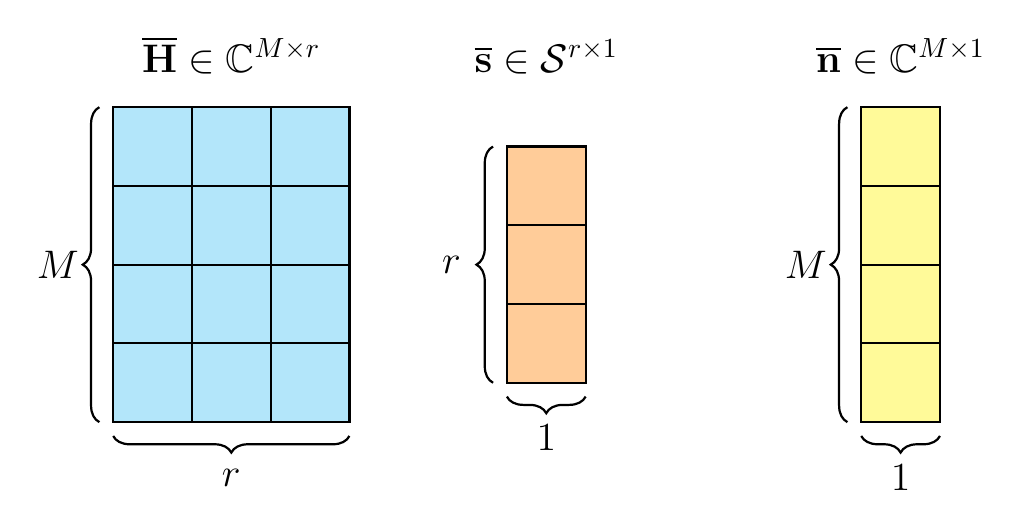
\begin{tikzpicture}[
cell/.style={draw, minimum size=1cm, inner sep=0pt, outer sep=0pt, thick},
brace/.style={decorate, decoration={brace, amplitude=6pt, raise=3pt}, thick}
]

% ==================== Matriz H (M x r) ====================
\begin{scope}[local bounding box=H]
\foreach \row in {1,...,4} {
\foreach \col in {1,...,3} {
\node[cell, fill=cyan!30] (H-\row-\col) at (\col*1, -\row*1) {};
}
}
\end{scope}
\node[above=0.3cm of H] {\Large $\overline{\mathbf{H}} \in \mathbb{C}^{M \times r}$};

% Chaves para H
\draw[brace] ([xshift=-2pt]H.south west) -- ([xshift=-2pt]H.north west) node[midway, xshift=-18pt] {\Large $M$};
\draw[brace] ([yshift=-2pt]H.south east) -- ([yshift=-2pt]H.south west) node[midway, yshift=-18pt] {\Large $r$};

% ==================== Vetor s (r x 1) ====================
\begin{scope}[local bounding box=s, xshift=5cm, yshift=-0.5cm]
\foreach \row in {1,...,3} {
\node[cell, fill=orange!40] (s-\row) at (1, -\row*1) {};
}
\end{scope}
\node[above=0.8cm of s] {\Large $\overline{\mathbf{s}} \in \mathcal{S}^{r \times 1}$};

% Chaves para s
\draw[brace] ([xshift=-2pt]s.south west) -- ([xshift=-2pt]s.north west) node[midway, xshift=-18pt] {\Large $r$};
\draw[brace] ([yshift=-2pt]s.south east) -- ([yshift=-2pt]s.south west) node[midway, yshift=-18pt] {\Large $1$};

% ==================== Vetor n (M x 1) ====================
\begin{scope}[local bounding box=n, xshift=9.5cm]
\foreach \row in {1,...,4} {
\node[cell, fill=yellow!40] (n-\row) at (1, -\row*1) {};
}
\end{scope}
\node[above=0.3cm of n] {\Large $\overline{\mathbf{n}} \in \mathbb{C}^{M \times 1}$};

% Chaves para n
\draw[brace] ([xshift=-2pt]n.south west) -- ([xshift=-2pt]n.north west) node[midway, xshift=-18pt] {\Large $M$};
\draw[brace] ([yshift=-2pt]n.south east) -- ([yshift=-2pt]n.south west) node[midway, yshift=-18pt] {\Large $1$};

\end{tikzpicture}%
}
\caption{Representação das dimensões das matrizes do sistema.}
\label{fig:matrizes}
\end{figure}


\subsection{\texorpdfstring{\textcolor{red}{Hipóteses do modelo}}{Hipóteses do modelo}}

Considera-se que os $r$ UEs não-alvo transmitem de forma independente entre si, com potência $\beta$, de modo que 

$$
\mathbb{E}[\overline{\mathbf{s}}\overline{\mathbf{s}}^H]=\beta\mathbf{I}_r
$$

Assume-se também que o ruído térmico é espacialmente branco, tal que 
$$\mathbb{E}[\overline{\mathbf{n}}\overline{\mathbf{n}}^H]=\sigma^2\mathbf{I}
$$ 

e que $\overline{\mathbf{s}}$ e $\overline{\mathbf{n}}$ são mutuamente independentes e possuem média nula. A matriz $\overline{\mathbf{H}}$ é considerada determinística, uma vez que permanece constante durante dado os mesmos parâmetros e entradas, isto é, no bloco de coerência,
% conforme será explicado posteriormente.
\textcolor{red}{conforme apresentado na Seção~{\hypersetup{linkcolor=red}\ref{subsec:bloco-coerencia}}.}

\begin{figure}[htbp]
\centering
\resizebox{0.8\textwidth}{!}{%
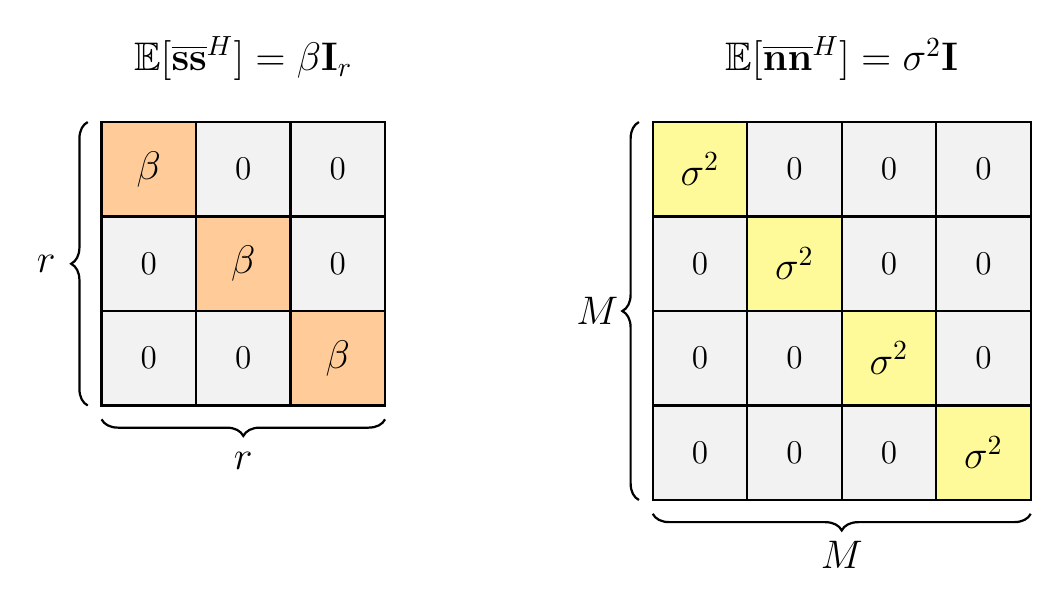
\begin{tikzpicture}[
cell/.style={draw, minimum size=1.2cm, inner sep=0pt, outer sep=0pt, thick},
brace/.style={decorate, decoration={brace, amplitude=6pt, raise=3pt}, thick}
]

% ==================== Matriz de Covariância de s (r x r) ====================
\begin{scope}[local bounding box=covS]
\foreach \row in {1,...,3} {
\foreach \col in {1,...,3} {
\ifnum\row=\col
\node[cell, fill=orange!40] (covS-\row-\col) at (\col*1.2, -\row*1.2) {\Large $\beta$};
\else
\node[cell, fill=black!5] (covS-\row-\col) at (\col*1.2, -\row*1.2) {\large $0$};
\fi
}
}
\end{scope}
\node[above=0.4cm of covS] {\Large $\mathbb{E}[\overline{\mathbf{s}}\overline{\mathbf{s}}^H] = \beta\mathbf{I}_r$};

% Chaves para a matriz de s
\draw[brace] ([xshift=-2pt]covS.south west) -- ([xshift=-2pt]covS.north west) node[midway, xshift=-18pt] {\Large $r$};
\draw[brace] ([yshift=-2pt]covS.south east) -- ([yshift=-2pt]covS.south west) node[midway, yshift=-18pt] {\Large $r$};

% ==================== Matriz de Covariância de n (M x M) ====================
\begin{scope}[local bounding box=covN, xshift=7cm]
\foreach \row in {1,...,4} {
\foreach \col in {1,...,4} {
\ifnum\row=\col
\node[cell, fill=yellow!40] (covN-\row-\col) at (\col*1.2, -\row*1.2) {\Large $\sigma^2$};
\else
\node[cell, fill=black!5] (covN-\row-\col) at (\col*1.2, -\row*1.2) {\large $0$};
\fi
}
}
\end{scope}
\node[above=0.4cm of covN] {\Large $\mathbb{E}[\overline{\mathbf{n}}\overline{\mathbf{n}}^H] = \sigma^2\mathbf{I}$};

% Chaves para a matriz de n
\draw[brace] ([xshift=-2pt]covN.south west) -- ([xshift=-2pt]covN.north west) node[midway, xshift=-18pt] {\Large $M$};
\draw[brace] ([yshift=-2pt]covN.south east) -- ([yshift=-2pt]covN.south west) node[midway, yshift=-18pt] {\Large $M$};

\end{tikzpicture}%
}
\caption{Matrizes de covariância dos sinais não-alvo e do ruído térmico espacialmente branco.}
\label{fig:covariancias}
\end{figure}


\subsection{\texorpdfstring{Construção de $\mathbf{R}_{\textcolor{red}{n}}$}{Construção de Rn}}\label{subsec:construcao-R}
\textcolor{red}{Esta seção constrói, para o cenário com interferência, a matriz $\mathbf{R}_n$ do equalizador LMMSE da Equação~{\hypersetup{linkcolor=red}\eqref{eq:mimo_correlations}}.}

Em uma transformação linear, em que um vetor aleatório $\mathbf{x}$ é obtido a partir de $\mathbf{z}$ por $\mathbf{x} = A\mathbf{z}$, com $A$ determinístico, a matriz de covariância de $\mathbf{x}$ pode ser obtida a partir da matriz de covariância de $\mathbf{z}$ por 

$$
\operatorname{Cov}(\mathbf{x}) = A\operatorname{Cov}(\mathbf{z})A^H,
$$

em que $A^H$ representa a transposta conjugada de $A$. Além disso, considerando duas variáveis aleatórias $\mathbf{u}$ e $\mathbf{v}$ independentes e de média zero, a matriz de covariância do vetor resultante da soma é dada por

$$
\operatorname{Cov}(\mathbf{u}+\mathbf{v})=\operatorname{Cov}(\mathbf{u})+\operatorname{Cov}(\mathbf{v}).
$$

A partir dessas hipóteses e do ruído colorido definido como $\mathbf{n}=\overline{\mathbf{H}}\overline{\mathbf{s}}+\overline{\mathbf{n}}$, as matrizes de covariância das parcelas $\overline{\mathbf{H}}\overline{\mathbf{s}}$ e $\overline{\mathbf{n}}$ podem ser somadas, pois são independentes e possuem média nula. Dessa forma,

$$
\mathbf{R}_{\textcolor{red}{n}}\triangleq\mathbb{E}[\mathbf{n}\mathbf{n}^H]
=\operatorname{Cov}(\overline{\mathbf{H}}\overline{\mathbf{s}})
+\operatorname{Cov}(\overline{\mathbf{n}}).
$$

A covariância da primeira parcela pode ser obtida pela propriedade da transformação linear, considerando $A=\overline{\mathbf{H}}$ e $\mathbf{z}=\overline{\mathbf{s}}$. Assim,

$$
\operatorname{Cov}(\overline{\mathbf{H}}\overline{\mathbf{s}})
=\overline{\mathbf{H}}\mathbb{E}[\overline{\mathbf{s}}\overline{\mathbf{s}}^H]\overline{\mathbf{H}}^H
=\beta\overline{\mathbf{H}}\overline{\mathbf{H}}^H.
$$

Como $\operatorname{Cov}(\overline{\mathbf{n}})=\sigma^2\mathbf{I}$, obtém-se, portanto, a matriz de covariância do ruído colorido:

$$
\mathbf{R}_{\textcolor{red}{n}}=\beta\overline{\mathbf{H}}\overline{\mathbf{H}}^H+\sigma^2\mathbf{I}.
$$

\textcolor{red}{Assim, no cenário com interferência, a matriz $\mathbf{R}_{yy}$ da Equação~{\hypersetup{linkcolor=red}\eqref{eq:mimo_correlations}} fica}

$$
\textcolor{red}{\mathbf{R}_{yy}=E_s\mathbf{H}\mathbf{H}^H+\beta\overline{\mathbf{H}}\overline{\mathbf{H}}^H+\sigma^2\mathbf{I}.}
$$


\begin{figure}[htbp]
\centering
\resizebox{\textwidth}{!}{%
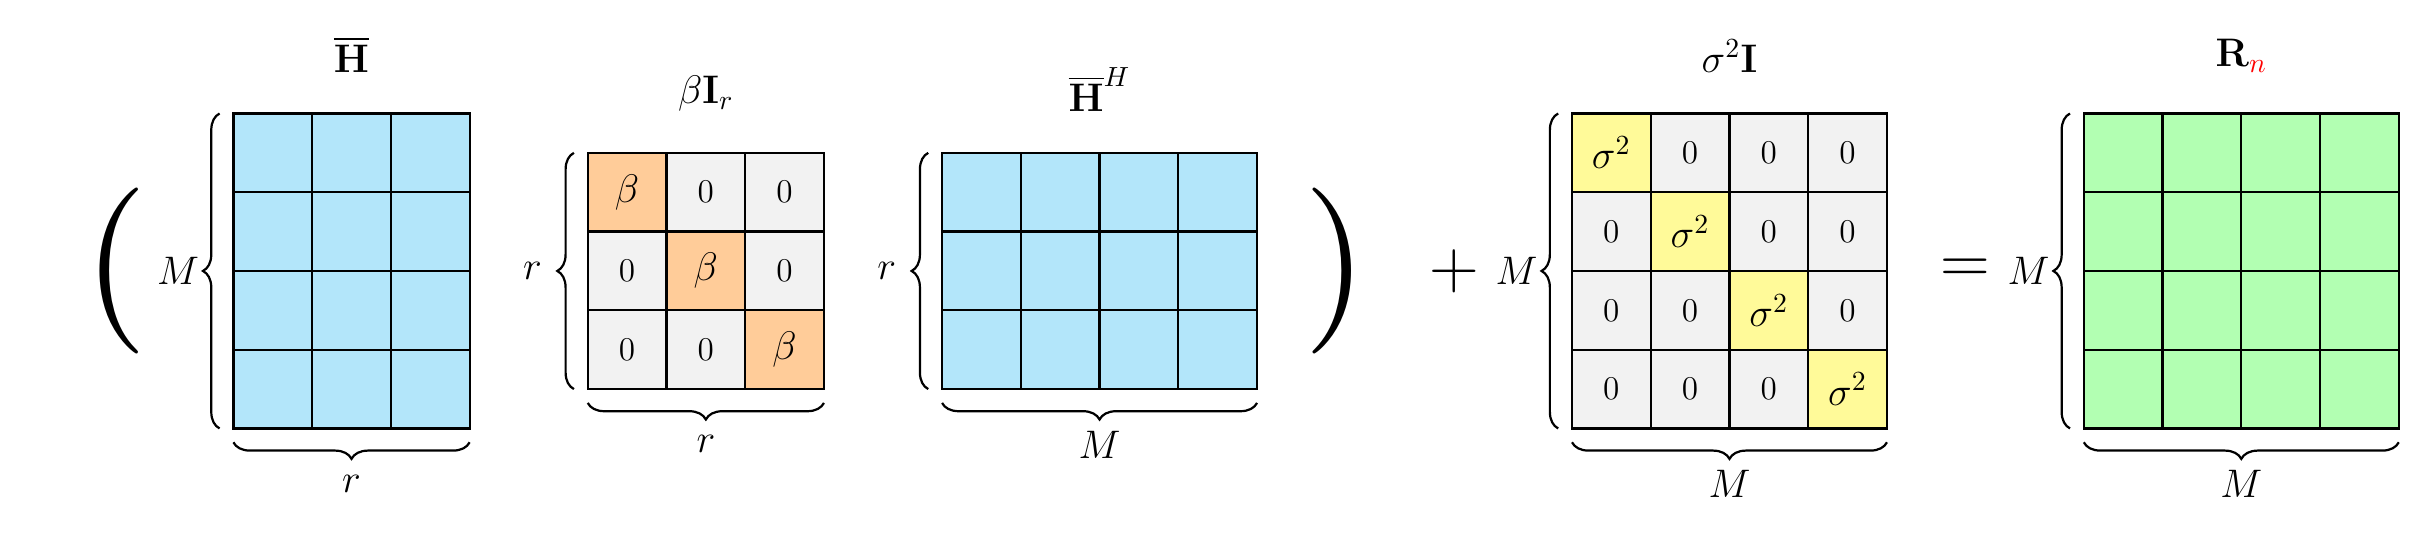
\begin{tikzpicture}[
    cell/.style={draw, minimum size=1cm, inner sep=0pt, outer sep=0pt, thick},
    brace/.style={decorate, decoration={brace, amplitude=6pt, raise=3pt}, thick}
]

% ==================== Parêntese Esquerdo ====================
\node[scale=6] at (0, -2.5) {$($};

% ==================== 1. Matriz H (M x r) ====================
\begin{scope}[local bounding box=Hbox, xshift=1cm]
    \foreach \row in {1,...,4} {
        \foreach \col in {1,...,3} {
            \node[cell, fill=cyan!30] (H-\row-\col) at (\col*1, -\row*1) {};
        }
    }
\end{scope}
\node[above=0.4cm of Hbox] {\Large $\overline{\mathbf{H}}$};
\draw[brace] ([xshift=-2pt]Hbox.south west) -- ([xshift=-2pt]Hbox.north west) node[midway, xshift=-18pt] {\Large $M$};
\draw[brace] ([yshift=-2pt]Hbox.south east) -- ([yshift=-2pt]Hbox.south west) node[midway, yshift=-18pt] {\Large $r$};

% ==================== 2. Matriz Beta (r x r) ====================
% xshift ajustado para 5.5cm (garante espaço perfeito para a chave esquerda)
\begin{scope}[local bounding box=betaBox, xshift=5.5cm, yshift=-0.5cm]
    \foreach \row in {1,...,3} {
        \foreach \col in {1,...,3} {
            \ifnum\row=\col
                \node[cell, fill=orange!40] (B-\row-\col) at (\col*1, -\row*1) {\Large $\beta$};
            \else
                \node[cell, fill=black!5] (B-\row-\col) at (\col*1, -\row*1) {\large $0$};
            \fi
        }
    }
\end{scope}
\node[above=0.4cm of betaBox] {\Large $\beta\mathbf{I}_r$};
\draw[brace] ([xshift=-2pt]betaBox.south west) -- ([xshift=-2pt]betaBox.north west) node[midway, xshift=-18pt] {\Large $r$};
\draw[brace] ([yshift=-2pt]betaBox.south east) -- ([yshift=-2pt]betaBox.south west) node[midway, yshift=-18pt] {\Large $r$};

% ==================== 3. Matriz H^H (r x M) ====================
% xshift ajustado para 10cm
\begin{scope}[local bounding box=HHbox, xshift=10cm, yshift=-0.5cm]
    \foreach \row in {1,...,3} {
        \foreach \col in {1,...,4} {
            \node[cell, fill=cyan!30] (HH-\row-\col) at (\col*1, -\row*1) {};
        }
    }
\end{scope}
\node[above=0.4cm of HHbox] {\Large $\overline{\mathbf{H}}^H$};
\draw[brace] ([xshift=-2pt]HHbox.south west) -- ([xshift=-2pt]HHbox.north west) node[midway, xshift=-18pt] {\Large $r$};
\draw[brace] ([yshift=-2pt]HHbox.south east) -- ([yshift=-2pt]HHbox.south west) node[midway, yshift=-18pt] {\Large $M$};

% ==================== Parêntese Direito ====================
\node[scale=6] at (15.5, -2.5) {$)$};

% ==================== Operador de Soma (+) ====================
\node at (17, -2.5) {\Huge $+$};

% ==================== 4. Matriz de Ruído Térmico (M x M) ====================
% xshift ajustado para 18cm
\begin{scope}[local bounding box=covN, xshift=18cm]
    \foreach \row in {1,...,4} {
        \foreach \col in {1,...,4} {
            \ifnum\row=\col
                \node[cell, fill=yellow!40] (t2-\row-\col) at (\col*1, -\row*1) {\Large $\sigma^2$};
            \else
                \node[cell, fill=black!5] (t2-\row-\col) at (\col*1, -\row*1) {\large $0$};
            \fi
        }
    }
\end{scope}
\node[above=0.4cm of covN] {\Large $\sigma^2\mathbf{I}$};
\draw[brace] ([xshift=-2pt]covN.south west) -- ([xshift=-2pt]covN.north west) node[midway, xshift=-18pt] {\Large $M$};
\draw[brace] ([yshift=-2pt]covN.south east) -- ([yshift=-2pt]covN.south west) node[midway, yshift=-18pt] {\Large $M$};

% ==================== Operador de Igualdade (=) ====================
\node at (23.5, -2.5) {\Huge $=$};

% ==================== 5. Matriz R (M x M) ====================
% xshift ajustado para 24.5cm
\begin{scope}[local bounding box=resultR, xshift=24.5cm]
    \foreach \row in {1,...,4} {
        \foreach \col in {1,...,4} {
            \node[cell, fill=green!30] (R-\row-\col) at (\col*1, -\row*1) {};
        }
    }
\end{scope}
\node[above=0.4cm of resultR] {\Large $\mathbf{R}_{\textcolor{red}{n}}$};
\draw[brace] ([xshift=-2pt]resultR.south west) -- ([xshift=-2pt]resultR.north west) node[midway, xshift=-18pt] {\Large $M$};
\draw[brace] ([yshift=-2pt]resultR.south east) -- ([yshift=-2pt]resultR.south west) node[midway, yshift=-18pt] {\Large $M$};

\end{tikzpicture}%
}
\caption{Formação da matriz de covariância do ruído colorido $\mathbf{R}_{\textcolor{red}{n}}$ a partir de seus fatores aditivos e multiplicativos.}
\label{fig:matriz_R}
\end{figure}

\subsection{Interferência sobre ruído térmico (IoT)}
% Novo: definição da IoT; papel de beta.

\subsection{\texorpdfstring{\textcolor{red}{O que $\mathbf{R}_n$ representa}}{O que Rn representa}}\label{subsec:o-que-R-representa}

% [ressaltar que a matriz de ruido eh MxM]

%% assim como tem a imagem das matrizes de covariancia e do ruido termico, mostrar como fica a matriz final, possivelmente fazer uma soma na figura dois 
A matriz $\mathbf{R}_{\textcolor{red}{n}}$ é composta por duas contribuições com características distintas. O termo $\sigma^2\mathbf{I}$ representa o ruído térmico. Como sua matriz de covariância possui apenas elementos na diagonal, o ruído presente em diferentes cadeias de recepção não é correlacionado. Já o termo $\beta\overline{\mathbf{H}}\overline{\mathbf{H}}^H$ representa a contribuição dos sinais transmitidos pelos UEs não-alvo após sua propagação pelo canal. Como cada um desses sinais é recebido por múltiplas antenas, o mesmo sinal pode contribuir para diferentes componentes do vetor recebido, estabelecendo uma relação entre elas. Dessa forma, essa parcela pode apresentar elementos fora da diagonal e introduzir correlação entre as antenas.

\section{\texorpdfstring{\textcolor{red}{Estimação de $\mathbf{R}_n$}}{Estimação de Rn}}
\label{sec:estimacao-R}
% CONTEÚDO  Roteiro T1: R não pode ser calculada; estimativa amostral com N
%           amostras de piloto; posto de R-chapéu; quantidade e custo de N.
% TEXTO     1-noise-and-constraints.tex, "Estimação de R_n" (subseções
%           parciais); constraints/rascunho_filtros_covariancia.tex.
% ESTADO    parcial

\subsection{\texorpdfstring{\textcolor{red}{Por que estimar $\mathbf{R}_n$}}{Por que estimar Rn}}

A matriz $\mathbf{R}_{\textcolor{red}{n}}$ descreve a matriz de covariância do ruído colorido completo, ou seja, a soma da interferência com o ruído térmico. Entretanto, não é possível obtê-la praticamente:  $\mathbb{E}[\cdot]$ é definida como uma média sobre infinitas realizações, desse modo, não é possível avaliar \textcolor{red}{$\mathbb{E}[\mathbf{n}\mathbf{n}^H]$} com um número finito de observações; além disso, $
\mathbf{R}_{\textcolor{red}{n}}=\beta\overline{\mathbf{H}}\overline{\mathbf{H}}^H+\sigma^2\mathbf{I}
$ depende das matrizes de canal $\overline{\mathbf{H}}$ das UEs não alvo, que não é estimada pelo receptor, assim como a potência $\beta$ de transmissão dos usuários não é. Dessa forma, $\mathbf{R}_{\textcolor{red}{n}}$ precisa ser estimada a partir de observações do próprio ruído. Essa estimativa é obtida através da média amostral

$$\hat{\mathbf{R}}_{\textcolor{red}{n}}=\frac{1}{N}\sum_{i=1}^{N}\mathbf{n}^i(\mathbf{n}^i)^H$$

em que \sout{$\mathbf{N}$} \textcolor{red}{$N$} é o número de amostras de ruído disponíveis.

\subsection{\texorpdfstring{\textcolor{red}{Como as amostras são obtidas}}{Como as amostras são obtidas}}
% Absorve a seção "Pilotos" (vazia) do capítulo atual.

As amostras de ruído são obtidas durante a etapa de símbolos piloto, sendo $\mathbf{n}^i \in \mathbb{C}^{M\times1}$ a amostra de ruído observada no $i$-ésimo elemento de recurso (RE) de piloto.  Nessa etapa, o sinal transmitido pelos UEs alvo é conhecido pelo receptor, e sua contribuição pode ser cancelada do sinal recebido. O que resta é o valor da interferência somada ao ruído térmico. 

\textcolor{red}{Cada amostra $\mathbf{n}^i$ é um vetor com um valor de ruído colorido para cada antena \cite{zhao2025jsac}. Assim, cada amostra é uma realização do mesmo ruído descrito pela matriz $\mathbf{R}_n$.}
% FONTE: artigo base, paper.md:123 (n^i em C^{M x 1}, amostra do i-ésimo RE de piloto).

\subsection{\texorpdfstring{\textcolor{red}{Intervalo das amostras}}{Intervalo das amostras}}

\textcolor{red}{Na frequência, a covariância do ruído permanece constante ao longo de um intervalo largo, e por isso pode ser estimada com uma média ao longo da frequência \cite{zhao2025jsac}. Assim, as amostras podem ser colhidas em REs de piloto de subportadoras diferentes. Para o canal, as respostas em frequências afastadas deixam de ser correlacionadas, e medir o canal em um conjunto suficiente de frequências permite estimar a sua covariância \cite{barriac-madhow}. Porém, é preciso haver subportadoras suficientes para que a estimativa se aproxime da covariância real \cite{barriac-madhow}.}
% FONTE: artigo base, nota 4 (paper.md:821, chamada em :115), que cita [29].
%        [29] Barriac e Madhow, pilot-estimation/Space*.md:96 e :109 (resultado para a
%        covariância do CANAL; a transferência para o ruído é feita pelo artigo base).

A média amostral é realizada uma vez por bloco de coerência e reutilizada ao longo dos $N_{\text{coh}}$ símbolos subsequentes, em que se assume que a covariância permanece estática.  

\textcolor{red}{Nesse intervalo, o canal e a covariância do ruído são considerados estáticos, e ambos mudam a cada novo bloco de coerência \cite{zhao2025jsac}. A estimativa obtida com os pilotos é usada para processar os sinais de dados recebidos em seguida \cite{tomasin-interference}. Para isso, a covariância precisa variar devagar o suficiente para que a estimativa ainda seja válida quando for usada \cite{barriac-madhow}.}
% FONTE: artigo base, paper.md:561; Tomasin et al. [22], pilot-estimation/Estimation*.md:68;
%        Barriac e Madhow [29], pilot-estimation/Space*.md:109, item (i).

\textcolor{red}{Dessa forma, as $N$ amostras são colhidas em REs de piloto dentro de um mesmo bloco de coerência. A estimativa $\hat{\mathbf{R}}_n$ obtida com elas vale para os $N_{\text{coh}}$ símbolos desse bloco.}
% FONTE: síntese de paper.md:123 (REs de piloto) e :561 (tempo).

\subsection{\texorpdfstring{\textcolor{red}{Uma estimativa por PRB}}{Uma estimativa por PRB}}\label{subsec:estimativa-prb}

\textcolor{red}{No artigo base, o PRB é a faixa de frequência e tempo em que o canal fica constante \cite{zhao2025jsac}. A matriz $\mathbf{R}_n = \beta\overline{\mathbf{H}}\overline{\mathbf{H}}^H+\sigma^2\mathbf{I}$ depende do canal $\overline{\mathbf{H}}$ dos UEs não-alvo \cite{zhao2025jsac}. Neste trabalho, considera-se que o canal dos UEs não-alvo também fica constante dentro do PRB. Assim, $\mathbf{R}_n$ também fica constante dentro do PRB, e muda de um PRB para outro.}
% FONTE: paper.md:614 (definição de PRB); paper.md:113 (R depende de Hbar).
% HIPÓTESE nossa: os interferentes têm o mesmo Doppler da condição de teste.

\textcolor{red}{Por isso, este trabalho usa uma estimativa $\hat{\mathbf{R}}_n$ para cada PRB, feita com $N$ amostras do próprio PRB. Esse é o modelo das simulações do artigo base, em que cada realização do canal tem $N = 192$ amostras de ruído \cite{zhao2025jsac}. O simulador deste trabalho segue o mesmo modelo: a cada realização, ele gera um novo $\overline{\mathbf{H}}$ e $N$ novas amostras de ruído.}
% FONTE: paper.md:577 (N = 192 por realização); simulador: dbp_sim/m1_driver.py:163-178
%        (Hbar e noise_samples gerados dentro do laço de realizações).

\textcolor{red}{A média ao longo da frequência, citada acima, seria uma alternativa: uma única estimativa para a banda inteira. Ela mudaria as curvas de SER, e por isso não é usada nos resultados.}
% FONTE: nota 4, paper.md:821. Decisão da autora (2026-10-12): modelo B (por PRB).
%        O modelo A fica como teste extra opcional (software/simulador_modelo_a).

\textcolor{red}{No tempo, o bloco de coerência tem a duração do tempo de coerência $T_c$ do canal. Neste trabalho, $T_c$ é calculado a partir do Doppler máximo $f_D$ de cada condição de teste \cite{3gpp-ts38104}, por $T_c = 1/(8 f_D)$ \cite[Eq.~2.44]{tse-viswanath}. As matrizes $\hat{\mathbf{R}}_n$, $\mathbf{G}_c$ e $\mathbf{W}$ são refeitas uma vez a cada $T_c$. Assim, $N_{\text{coh}}$ é o número de símbolos OFDM em $T_c$.}
% FONTE: f_D: [R5] TS 38.104 v16.4.0, Anexo G, Tab. G.2.2-1, G.2.2-2 (p. 241), G.3-1 e
%        G.3-2 (p. 252); T_c = 1/(4 D_s) = 1/(8 f_D): Tse e Viswanath, Eq. (2.44), p. 31.
%        Refazer a cada T_c: decisão da autora, opção (b), apoiada em paper.md:614.
%        Valores de T_c e símbolos por T_c: software/Restrições - Parâmetros.csv, linhas 17-24.

\subsection{\texorpdfstring{\textcolor{red}{O que cada amostra contribui}}{O que cada amostra contribui}}

\textcolor{red}{A Figura~{\hypersetup{linkcolor=red}\ref{fig:posto_unitario}} mostra a parcela $\mathbf{n}^i(\mathbf{n}^i)^H$ referente a uma única amostra de ruído.}

\begin{figure}[htbp]
\centering
\resizebox{\textwidth}{!}{%
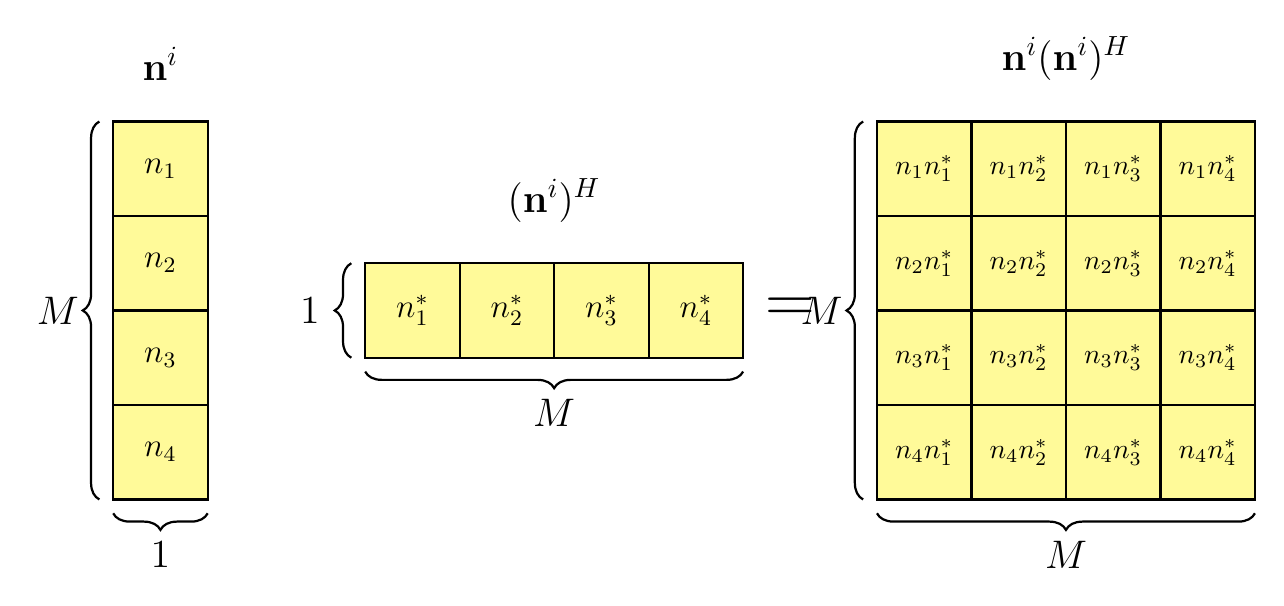
\begin{tikzpicture}[
    cell/.style={draw, minimum size=1.2cm, inner sep=0pt, outer sep=0pt, thick},
    brace/.style={decorate, decoration={brace, amplitude=6pt, raise=3pt}, thick}
]

% ==================== 1. Vetor Coluna n^i (M x 1) ====================
\begin{scope}[local bounding box=ni]
    \foreach \row in {1,...,4} {
        \node[cell, fill=yellow!40] (ni-\row) at (0, -\row*1.2) {\large $n_\row$};
    }
\end{scope}
\node[above=0.4cm of ni] {\Large $\mathbf{n}^i$};

\draw[brace] ([xshift=-2pt]ni.south west) -- ([xshift=-2pt]ni.north west) node[midway, xshift=-18pt] {\Large $M$};
\draw[brace] ([yshift=-2pt]ni.south east) -- ([yshift=-2pt]ni.south west) node[midway, yshift=-18pt] {\Large $1$};

% ==================== 2. Vetor Linha (n^i)^H (1 x M) ====================
\begin{scope}[local bounding box=nih, xshift=2cm]
    \foreach \col in {1,...,4} {
        % O vetor linha é centralizado verticalmente em relacao ao vetor coluna (y=-3.0 corresponde ao meio)
        \node[cell, fill=yellow!40] (nih-\col) at (\col*1.2, -3.0) {\large $n_\col^*$}; 
    }
\end{scope}
\node[above=0.4cm of nih] {\Large $(\mathbf{n}^i)^H$};

\draw[brace] ([xshift=-2pt]nih.south west) -- ([xshift=-2pt]nih.north west) node[midway, xshift=-18pt] {\Large $1$};
\draw[brace] ([yshift=-2pt]nih.south east) -- ([yshift=-2pt]nih.south west) node[midway, yshift=-18pt] {\Large $M$};

% ==================== Operador de Igualdade (=) ====================
\node at (8.0, -3.0) {\Huge $=$};

% ==================== 3. Matriz Resultante (M x M) ====================
\begin{scope}[local bounding box=ni_result, xshift=8.5cm]
    \foreach \row in {1,...,4} {
        \foreach \col in {1,...,4} {
            \node[cell, fill=yellow!40] (res-\row-\col) at (\col*1.2, -\row*1.2) {\normalsize $n_\row n_\col^*$};
        }
    }
\end{scope}
\node[above=0.4cm of ni_result] {\Large $\mathbf{n}^i(\mathbf{n}^i)^H$};

\draw[brace] ([xshift=-2pt]ni_result.south west) -- ([xshift=-2pt]ni_result.north west) node[midway, xshift=-18pt] {\Large $M$};
\draw[brace] ([yshift=-2pt]ni_result.south east) -- ([yshift=-2pt]ni_result.south west) node[midway, yshift=-18pt] {\Large $M$};

\end{tikzpicture}%
}
\caption{Dimensões do produto externo para a parcela da estimativa da matriz de covariância.}
\label{fig:posto_unitario}
\end{figure}

Como cada celula representa
% a interfencia de uma antena em outra,
\textcolor{red}{o produto $n_a n_b^*$ entre o ruído observado na antena $a$ e o ruído observado na antena $b$ em uma mesma amostra, a média dessas células ao longo das $N$ amostras se aproxima do elemento correspondente de $\mathbf{R}_n$, que indica o quanto o ruído dessas duas antenas varia em conjunto.}

O posto de uma matriz é o número máximo de linhas ou colunas linearmente independentes que essa matriz possui.  Cada parcela $\mathbf{n}^i(\mathbf{n}^i)^H$ é uma matriz de posto unitário, uma vez que todas as suas colunas são múltiplas do mesmo vetor $\mathbf{n}^i$.

\textcolor{red}{Uma única amostra mostra apenas uma realização do ruído. Calcular o produto para várias realizações independentes e tirar a média desses produtos resulta em uma estimativa da correlação \cite[p.~229]{haykin-sistemas}. Essa estimativa se aproxima de $\mathbf{R}_n$ conforme o número de amostras cresce, mas essa convergência é lenta \cite{tomasin-interference}.}
% FONTE: livro de probabilidade, Exemplo 5.16, p. 229; Tomasin et al. [22], Estimation*.md:109.

\subsection{\texorpdfstring{\textcolor{red}{Quantidade de amostras}}{Quantidade de amostras}}
% Posto de R-chapéu <= N: motiva o condicionamento (subseção seguinte).

\textcolor{red}{O erro quadrático médio de cada elemento de $\hat{\mathbf{R}}_n$ diminui na proporção de $1/N$, considerando amostras gaussianas e independentes entre si \cite{tomasin-interference}. Assim, quanto maior o número de amostras, mais precisa é a estimativa. Por isso, o artigo base exige $N \gg K$, para garantir a acurácia da estimativa \cite{zhao2025jsac}. Quando $N$ é grande, o erro entre $\hat{\mathbf{R}}_n$ e $\mathbf{R}_n$ é pequeno \cite{zhao2025jsac}.}
% FONTE: Tomasin et al. [22], eq. (21)-(23), Estimation*.md:242-259 (hipóteses em :57 e :246);
%        artigo base, paper.md:123 (N >> K) e nota 5, paper.md:821.

\textcolor{red}{Nas simulações, o artigo base usa $N = 192$ \cite{zhao2025jsac}. Um trabalho anterior dos mesmos autores cita 96 ou 192 como valores típicos de $N$ \cite{zhao2021-globecom}. Como as amostras vêm dos REs de piloto do PRB, $N$ também fica limitado ao número de REs de piloto que cabem em $T_c$.}
% FONTE: paper.md:577 e :640 (N = 192); zhao2021_globecom, linha 54 ("typically 96 or 192").
% NOTA: a última frase é dedução (paper.md:123 + :614).

\subsection{\texorpdfstring{\textcolor{red}{REs de piloto disponíveis}}{REs de piloto disponíveis}}\label{subsec:res-piloto}

\textcolor{red}{Neste trabalho, as amostras de ruído vêm dos REs do sinal de referência de demodulação (DM-RS). Um PRB tem 12 subportadoras \cite[Sec.~4.4.4.1]{3gpp-ts38211}, e um slot tem 14 símbolos OFDM \cite[Tab.~4.3.2-1]{3gpp-ts38211}. O DM-RS ocupa no máximo 4 símbolos por slot \cite[Tab.~6.4.1.1.3-3 e 6.4.1.1.3-4]{3gpp-ts38211}. Assim, cabem no máximo $4 \times 12 = 48$ REs de DM-RS por PRB em um slot. Para juntar $N = 192$ amostras, são precisos pelo menos 4 slots.}
% FONTE: [R2] TS 38.211 v18.6.0: Sec. 4.4.4.1, p. 15 (12 subportadoras); Tab. 4.3.2-1,
%        p. 14 (14 símbolos por slot); Tab. 6.4.1.1.3-3 e -4, p. 101 (até 4 símbolos de DM-RS).
% HIPÓTESE nossa: contar só o DM-RS. O artigo diz apenas "pilot REs" (paper.md:123).
%        O SRS poderia dar mais REs ([R2] Sec. 6.4.1.4.1, p. 109-110), mas não é usado.

\textcolor{red}{A Tabela~{\hypersetup{linkcolor=red}\ref{tab:n-maximo}} mostra quantos REs de DM-RS cabem em um PRB dentro de $T_c$, para cada condição de teste. Nas condições mais lentas, as 192 amostras cabem em $T_c$. Nas mais rápidas, não cabem, e $N$ fica limitado ao número máximo de REs. Nos trens de alta velocidade, cabe só um símbolo OFDM inteiro em $T_c$, e restam 12 REs.}
% FONTE: software/Restrições - Parâmetros.csv, tabela "Número máximo de REs de piloto
%        (DM-RS) por PRB em T_c" (linhas 44-53). Símbolos de DM-RS em S símbolos:
%        4*floor(S/14) + min(S mod 14, 4).

\begin{table}[htbp]
\caption{\textcolor{red}{Número máximo de REs de DM-RS por PRB dentro de $T_c$.}}
\label{tab:n-maximo}
\centering
\footnotesize
\renewcommand{\arraystretch}{1.2}
\begin{tabular}{|l|r|r|r|r|}
\hline
Condição de teste & $T_c$ (ms) & Símbolos OFDM em $T_c$ & REs de DM-RS (máx.) & $N$ usado \\
\hline
TDLA30-5 (FR1)    & 25,0000 & 700 & 2400 & 192 \\
TDLA30-10 (FR1)   & 12,5000 & 350 & 1200 & 192 \\
TDLA30-75 (FR2)   & 1,6667  & 186 & 672  & 192 \\
TDLA30-300 (FR2)  & 0,4167  & 46  & 192  & 192 \\
TDLC300-100 (FR1) & 1,2500  & 35  & 144  & 144 \\
TDLB100-400 (FR1) & 0,3125  & 8   & 48   & 48 \\
HST350 (FR1)      & 0,0536  & 1   & 12   & 12 \\
HST500 (FR1)      & 0,0375  & 1   & 12   & 12 \\
\hline
\end{tabular}
\end{table}
% FONTE da tabela: f_D e condições: [R5] Anexo G; T_c: Tse e Viswanath, Eq. (2.44);
%        símbolo OFDM: 1/28 ms (30 kHz) e 1/112 ms (120 kHz), [R2] Tab. 4.3.2-1, p. 14.

\textcolor{red}{Essa limitação vale para um receptor em tempo real. A simulação não tem tempo: cada realização é um instante isolado, com $N$ amostras próprias. Por isso, as curvas de SER com $N = 192$ continuam válidas como no artigo base. Para ver o efeito de um $N$ menor, este trabalho propõe testes extras com $N = 12$, 48, 96, 144 e 192.}
% FONTE: dbp_sim/m1_driver.py:163-178 (sem eixo de tempo); dbp_sim/params.py:302 (N = 192).
% ESTADO: testes com N diferente ainda não rodados (falta a opção --n-noise-samples).

\subsection{Condicionamento da estimativa}\label{subsec:condicionamento-R}
% CONTEÚDO  Quando N < M, o posto de R-chapéu é no máximo N e a matriz não
%           tem inversa (M = 256, N = 192). O LMMSE precisa dessa inversa.
%           Shrinkage de Ledoit-Wolf: R-chapéu vira (1 - rho) R-chapéu +
%           rho (tr R-chapéu / M) I, com rho calculado a partir das próprias
%           amostras (sem constante a escolher). Alternativa: carga diagonal
%           fixa, que depende de um epsilon.
% TEXTO     nenhum na fundamentação; parágrafo sobre Ledoit-Wolf em
%           rascunho_setup_simulacao.tex (subseção Receptor);
%           dbp_sim/params.py, M6_Covariance.shrinkage.
% FONTE     Ledoit e Wolf (2004), J. Multivariate Analysis 88(2) -- falta
%           no .bib; posto <= N: livro-texto de álgebra linear.
% MÓDULO    M6 (Conditioner em dbp_sim/m5_noise.py)
% ESTADO    a escrever

\textcolor{red}{Cada parcela $\mathbf{n}^i(\mathbf{n}^i)^H$ tem posto unitário. Por isso, a soma de $N$ parcelas tem posto de no máximo $N$. Nas DUs, a estimativa de cada bloco tem tamanho $M_c \times M_c$ (Seção~{\hypersetup{linkcolor=red}\ref{subsec:estimacao-dus}}). Com $N = 192$, o posto não limita o bloco, pois $M_c$ vale 8, 16 ou 32 \cite{zhao2025jsac}. Já nas condições rápidas da Tabela~{\hypersetup{linkcolor=red}\ref{tab:n-maximo}}, $N$ pode ser 12. Nesse caso, um bloco com $M_c = 16$ tem posto de no máximo 12 e não tem inversa. Além disso, $N = 12$ não atende $N \gg K$, com $K = 8$ \cite{zhao2025jsac}. Este trabalho usa o encolhimento de Ledoit-Wolf em cada bloco, que mantém a matriz inversível \cite{ledoit-wolf}.}
% FONTE: posto unitário: parágrafo anterior desta seção; M_c = M/C com M = 128 ou 256 e
%        C = 8 ou 16: paper.md:577; N >> K: paper.md:123; Ledoit-Wolf por bloco:
%        dbp_sim/m5_noise.py:159-168 (Conditioner.covariance), dbp_sim/m7_equalizers.py:71,
%        dbp_sim/params.py:334.
% NOTA: quando N < M_c, o simulador não calcula rho no bloco; usa a intensidade calculada
%        com a matriz de amostras inteira (m5_noise.py:154-157 e :166-167).
% FALTA no biblio.bib: ledoit-wolf (Ledoit e Wolf, 2004, J. Multivariate Analysis 88(2)).

\subsection{\texorpdfstring{\textcolor{red}{Custo do N}}{Custo do N}}

\textcolor{red}{Por outro lado, um $N$ maior aumenta a quantidade de dados que precisa ser guardada e transmitida. Cada DU guarda as $N$ amostras de ruído das suas antenas \cite{zhao2025jsac}. Trocar essas amostras entre as DUs exigiria transferir dados de tamanho $M \times N$ \cite{zhao2025jsac}. No BCD-MMSE, a banda de comunicação em cada iteração ainda depende de $N$ \cite{zhao2025jsac}. Como a estimativa só muda a cada bloco de coerência, esse custo é pago uma vez a cada $N_{\text{coh}}$ símbolos \cite{zhao2025jsac}.}
% FONTE: artigo base, paper.md:493 (N_c em C^{M_c x N} guardado na DU c); :130 (M x N);
%        :471 (banda por iteração depende de N); :561 e :571 (termos divididos por N_coh).

\textcolor{red}{Um $N$ maior também leva mais tempo para ser juntado. Com 48 REs de DM-RS por PRB em cada slot (Seção~{\hypersetup{linkcolor=red}\ref{subsec:res-piloto}}), o tempo de coleta das $N$ amostras é}
\begin{equation*}
\textcolor{red}{t_{\text{coleta}} = \min\left(T_c;\ \left\lceil \frac{N}{48} \right\rceil \text{ slots}\right).}
\end{equation*}
\textcolor{red}{Com $N = 192$, são 4 slots: 2~ms em FR1, com slots de 0,5~ms, e 0,5~ms em FR2, com slots de 0,125~ms \cite[Tab.~4.3.2-1]{3gpp-ts38211}. Nas condições rápidas, as amostras ocupam o $T_c$ inteiro.}
% FONTE: slot de 0,5 ms (mu = 1, 30 kHz) e 0,125 ms (mu = 3, 120 kHz): [R2] Tab. 4.3.2-1,
%        p. 14. Regra de t_coleta: conta nossa; planilha, linhas 67-76.

\textcolor{red}{A estimativa só fica pronta depois da coleta. Por isso, este trabalho considera um processamento em etapas (\textit{pipeline}). Enquanto junta as amostras de um bloco, a DU guarda os dados recebidos nesse bloco. Depois, calcula $\hat{\mathbf{R}}_n$, $\mathbf{G}_c$ e $\mathbf{W}$ e equaliza os dados guardados. Ao mesmo tempo, já junta as amostras do bloco seguinte. Assim, o cálculo de cada bloco precisa terminar em até $T_c$. O tempo total, da primeira amostra até o resultado, é $t_{\text{coleta}} + t_{\text{proc}}$, em que $t_{\text{proc}}$ é o tempo de cálculo.}
% FONTE: decisão da autora (2026-10-12). Condições t_proc <= T_c e t_coleta + t_proc <= D:
%        planilha, tabela "Fórmulas de latência". D fica só como fórmula (sem fonte).
%        Os dados guardados seguem paper.md:561 (W reutilizado nos N_coh símbolos).

\section{Definição Decentralizada}
\label{sec:dbp}
% CONTEÚDO  Arquitetura DBP: clusters, DUs, CU; estrela e daisy chain;
%           roteiro T2 (o que cada DU alcança) e T3 (a bifurcação: descartar
%           os blocos cruzados -> BDAC; mantê-los comprimidos -> BCD).
% TEXTO     1-noise-and-constraints.tex, "Definição Decentralizada" (vazia)
%           e "Estimação nas DUs" (2 linhas).
% ESTADO    vazio



\subsection{Arquitetura e particionamento das antenas}

\subsection{\texorpdfstring{\textcolor{red}{Estimação nas DUs}}{Estimação nas DUs}}\label{subsec:estimacao-dus}

\textcolor{red}{Conforme apresentado na Seção~{\hypersetup{linkcolor=red}\ref{subsec:o-que-R-representa}}, a parcela $\beta\overline{\mathbf{H}}\overline{\mathbf{H}}^H$ introduz correlação entre as antenas.}
%% TIRAR DAQUI E DILUIR NO RESTO DO TESTO OU POR DEPOIS 
Essa correlação tem uma consequência importante para a arquitetura considerada. Ao particionar as antenas em diferentes clusters associados às DUs, a matriz $\mathbf{R}_{\textcolor{red}{n}}$, em geral, não possui estrutura bloco-diagonal. Assim, os blocos fora da diagonal, dados por $\mathbf{R}_{mn}=\mathbb{E}[\mathbf{n}_m\mathbf{n}_n^H]$, representam a correlação entre os sinais de ruído observados por antenas pertencentes a DUs distintas. Para obter essas correlações diretamente a partir das amostras de ruído, seria necessário compartilhar informações entre as unidades, aumentando o tráfego de comunicação.

\textcolor{red}{Cada amostra $\mathbf{n}^i$ pode ser dividida em partes $\mathbf{n}_c^i$, uma para cada cluster, e a DU $c$ guarda apenas as amostras das suas próprias antenas \cite{zhao2025jsac}. Com elas, a DU $c$ calcula, sem trocar dados, só o bloco da diagonal}
\begin{equation*}
\textcolor{red}{\hat{\mathbf{R}}_{cc}=\frac{1}{N}\sum_{i=1}^{N}\mathbf{n}_c^i(\mathbf{n}_c^i)^H,}
\end{equation*}
\textcolor{red}{de tamanho $M_c \times M_c$. Os blocos fora da diagonal precisariam de amostras de outras DUs \cite{zhao2025jsac}. Neste trabalho, cada DU aplica o encolhimento de Ledoit-Wolf ao seu próprio bloco (Seção~{\hypersetup{linkcolor=red}\ref{subsec:condicionamento-R}}).}
% FONTE: paper.md:123-125 (n^i dividido em n_c^i, guardado no cluster c; R_mn = E[n_m n_n^H]);
%        Fig. 3 e paper.md:128 (blocos fora da diagonal exigem troca de dados);
%        LW por bloco: dbp_sim/m7_equalizers.py:71.

\textcolor{red}{No BCD-MMSE, a DU $c$ usa $\hat{\mathbf{R}}_{cc}$ de duas formas. Na inicialização, usa a inversa $\hat{\mathbf{R}}_{cc}^{-1}$, pois o BCD-MMSE começa pela aproximação bloco-diagonal \cite{zhao2025jsac}. Nas iterações, soma $\hat{\mathbf{R}}_{cc}$ ao termo do canal e forma a matriz $\mathbf{G}_c = E_s\mathbf{H}_c\mathbf{H}_c^H + \hat{\mathbf{R}}_{cc}$, que é invertida \cite{zhao2025jsac}. $\mathbf{G}_c$ usa $\hat{\mathbf{R}}_{cc}$, e não a sua inversa. Por isso, as duas inversões podem ser feitas em paralelo.}
% FONTE: Algoritmo 3, paper.md:415 (W^0 pela Eq. 7); Eq. 7, paper.md:136-142 (R_cc^-1);
%        Eq. 30, paper.md:504 (G_c com (1/N) sum n_c^i (n_c^i)^H).
%        G_c^-1 é calculada uma vez por PRB e reutilizada nas T iterações (não muda com l).

\textcolor{red}{Como há uma estimativa por PRB (Seção~{\hypersetup{linkcolor=red}\ref{subsec:estimativa-prb}}), cada DU calcula, a cada $T_c$, $N_{\text{PRB}}$ estimativas $\hat{\mathbf{R}}_{cc}$, $N_{\text{PRB}}$ inversões de $\hat{\mathbf{R}}_{cc}$ e $N_{\text{PRB}}$ inversões de $\mathbf{G}_c$. Com o pior caso do artigo base, $N_{\text{PRB}} = 275$ \cite{zhao2025jsac}.}
% FONTE: N_PRB = 275: paper.md:640. Contagem: planilha, tabela "Carga por PRB" (linhas 56-66).
% O que cada DU tem aceso

% É iniciado como bloco diagonal

\subsection{Aproximação bloco-diagonal (BDAC-MMSE)}

\section{Equalizador BCD-MMSE}\label{sec:bcd}
% CONTEÚDO  Roteiro T4 (formulação BCD), T5 (da eq. 26 à eq. 30) e T6 (o
%           fator a inverter, G_c = E_s H_c H_c^H + R_cc, e suas
%           propriedades: hermitiana, definida positiva).
% TEXTO     constraints/notas_redacao.md (T4-T6);
%           constraints/modelo_ruido_e_hipoteses.md, seção 10.
% ESTADO    a escrever

\subsection{Formulação por blocos}

\subsection{Atualização de cada DU}

\subsection{A matriz invertida em cada DU}\label{subsec:Gc}

\section{Inversão de matrizes}
% CONTEÚDO  Custo O(M_c^3); decomposição de Cholesky para matrizes
%           hermitianas definidas positivas; substituições direta e reversa;
%           série de Neumann e outras alternativas; por que Cholesky para G_c.
% TEXTO     Proposta do TG1, "Matrix Inversion Techniques".
% ESTADO    a escrever (traduzir e adaptar)

\subsection{Decomposição de Cholesky}

\subsection{Série de Neumann}

\subsection{Comparação}

\section{Extração de Parâmetros}


% referências
% aqui será usado o environment padrao `thebibliography'; porém, sugere-se
% seriamente o uso de BibTeX e do estilo abnt.bst (veja na página do
% UTUG)
% 
% observe também o estilo meio estranho de alguns labels; isso é
% devido ao uso do pacote `natbib', que permite fazer citações de
% autores, ano, e diversas combinações desses

\bibliographystyle{abntex2-alf}
\bibliography{biblio}

\end{document}
